\setcounter{errorcontextlines}{5}

\documentclass[12pt]{book}


%% Do I need to define Internet?
%% Do I need to define Internet Service Provider?
%% Do I need to describe WiFi and Ethernet?

% FIXME - need to check line breaks in program code before shipping
% FIXME - enter vs return key
% FIXME - special values such as NaN, null, undefined, and Infinity

\usepackage[top=1in,bottom=0.5in,left=0.5in,right=0.5in, paperwidth=7.5in, paperheight=9.25in]{geometry}
%\usepackage[margin=1in, paperwidth=8.5in, paperheight=11in]{geometry}
\usepackage{graphicx}
\usepackage{mdframed}
\usepackage{xcolor}
\usepackage[T1]{fontenc}
\usepackage[utf8]{inputenc}
\usepackage{nicefrac}
\usepackage{graphicx}
\usepackage{mdframed}
\usepackage{float}
\usepackage{placeins}
\usepackage{hyperref}
\usepackage{needspace}
\usepackage{dingbat}
\usepackage{listings}
\newcommand{\UnderscoreCommands}{\do\lstinputlisting}

\makeatletter
\@ifpackageloaded{tex4ht}{
\usepackage[english]{babel} % Prevents underscore from causing problems with tex4ht - in the future I should include this by default before all of my checking, but since I have already proofed without it, I don't want to screw anything up.
\newcommand{\forebook}[1]{#1}
\newcommand{\forprintbook}[1]{}
}{
\newcommand{\forebook}[1]{}
\newcommand{\forprintbook}[1]{#1}
}
\makeatother

\usepackage[strings]{underscore}

\setcounter{tocdepth}{1}
\setlength{\parindent}{0in}
\setlength{\parskip}{12pt}

\lstset{ %
basicstyle=\ttfamily,
breakatwhitespace=true,
breaklines=true,
tabsize=3
}

\forprintbook{
\def\bookpart#1{%
  \par\newpage\cleardoublepage % Page break
  \thispagestyle{empty}
  \chaptermark{~}
  \sectionmark{~}
  \markboth{~}{~}
  \vspace*{1in} % Vertical shift
  \refstepcounter{part}% Next part
  {\centering\textbf{\Huge Part \thepart}\par}% 
  \addcontentsline{toc}{part}{{\thepart}~~~~~#1}
  \vspace{1cm}% Vertical shift
  {\centering \textbf{\Huge #1}\par}%
  \vspace{2cm}% Vertical shift
  % Some text
}
}

\forebook{
\def\bookpart#1{%
%\section*{~}
%\refstepcounter{part}% Next part
%{\centering\textbf{\Huge Part \thepart}\par}% 
% \part{#1}
% \addcontentsline{toc}{part}{{\thepart}~~~~~#1}
}
}

\forprintbook{
\newenvironment{partintro}{\begin{mdframed}[backgroundcolor=gray!10,skipabove=\baselineskip,skipbelow=\baselineskip]%
~\\ 
}{%
~\\
\end{mdframed}
}
}

\forebook{
\newenvironment{partintro}{}{}
}

\newcommand{\eaxReg}{\icode{\%eax}}
\newcommand{\eaxRegIdx}{\icode{\%eax}\index{\%eax}}
\newcommand{\eaxBare}{\%eax}
\newcommand{\ebxReg}{\icode{\%ebx}}
\newcommand{\ebxRegIdx}{\icode{\%ebx}\index{\%ebx}}
\newcommand{\ebxBare}{\%ebx}
\newcommand{\ecxReg}{\icode{\%ecx}}
\newcommand{\ecxRegIdx}{\icode{\%ecx}\index{\%ecx}}
\newcommand{\ecxBare}{\%ecx}
\newcommand{\edxReg}{\icode{\%edx}}
\newcommand{\edxRegIdx}{\icode{\%edx}\index{\%edx}}
\newcommand{\edxBare}{\%edx}
\newcommand{\ediReg}{\icode{\%edi}}
\newcommand{\ediRegIdx}{\icode{\%edi}\index{\%edi}}
\newcommand{\ediBare}{\%edi}
\newcommand{\esiReg}{\icode{\%esi}}
\newcommand{\esiRegIdx}{\icode{\%esi}\index{\%esi}}
\newcommand{\esiBare}{\%esi}
\newcommand{\ebpReg}{\icode{\%ebp}}
\newcommand{\ebpRegIdx}{\icode{\%ebp}\index{\%ebp}}
\newcommand{\ebpBare}{\%ebp}
\newcommand{\espReg}{\icode{\%esp}}
\newcommand{\espRegIdx}{\icode{\%esp}\index{\%esp}}
\newcommand{\espBare}{\%esp}
\newcommand{\eflagsReg}{\icode{\%eflags}}
\newcommand{\eflagsRegIdx}{\icode{\%eflags}\index{\%eflags}}
\newcommand{\eflagsBare}{\%eflags}
\newcommand{\eipReg}{\icode{\%eip}}
\newcommand{\eipRegIdx}{\icode{\%eip}\index{\%eip}}
\newcommand{\eipBare}{\%eip}
\newcommand{\raxReg}{\icode{\%rax}}
\newcommand{\raxRegIdx}{\icode{\%rax}\index{\%rax}}
\newcommand{\raxBare}{\%ax}
\newcommand{\axReg}{\icode{\%ax}}
\newcommand{\axRegIdx}{\icode{\%ax}\index{\%ax}}
\newcommand{\axBare}{\%ax}
\newcommand{\alReg}{\icode{\%al}}
\newcommand{\alRegIdx}{\icode{\%al}\index{\%al}}
\newcommand{\alBare}{\%al}
\newcommand{\ahReg}{\icode{\%ah}}
\newcommand{\ahRegIdx}{\icode{\%ah}\index{\%ah}}
\newcommand{\ahBare}{\%ah}
\newcommand{\clReg}{\icode{\%cl}}
\newcommand{\clRegIdx}{\icode{\%cl}\index{\%cl}}
\newcommand{\clBare}{\%al}

\newcommand{\icodefilename}[1]{\icode{#1}}

\newcommand{\minstruction}[1]{\mbox{\texttt{#1}}}

\newcommand{\reviewsection}{\newpage \section*{Review}}
\newcommand{\applysection}{\section*{Apply What You Have Learned}}
\newcommand{\glossterm}[1]{\textbf{#1}}
\newcommand{\latinphrase}[1]{\textit{#1}}
\newcommand{\icode}[1]{\texttt{\mbox{#1}}}
\newcommand{\documentname}[1]{\emph{#1}}
\newcommand{\jskw}[1]{\texttt{\mbox{#1}}}
\newcommand{\jsoper}[1]{\texttt{\mbox{#1}}}
\newcommand{\stdfunc}[1]{\texttt{\mbox{#1}}}
\newcommand{\stdclass}[1]{\texttt{\mbox{#1}}}
\newcommand{\stdprop}[1]{\texttt{\mbox{#1}}}
\newcommand{\htmlattr}[1]{\texttt{\mbox{#1}}}
\newcommand{\stdobj}[1]{\texttt{\mbox{#1}}}
\newcommand{\tag}[1]{\icode{\mbox{<#1>}}}
\newcommand{\hent}[1]{\icode{\mbox{\&#1;}}}

\newenvironment{classdoc}[1]{\begin{figure}[H] \caption{The \stdclass{#1} Class}}{\end{figure}}
\newenvironment{propdoc}{\textbf{Properties:} \\ \begin{tabular}{| p{0.4\textwidth} | p{0.6\textwidth} |} \hline}{\hline \end{tabular}}
\newenvironment{methdoc}{\\ \\ \textbf{Methods:} \\ \begin{tabular}{| p{0.4\textwidth} | p{0.6\textwidth} |} \hline}{\hline \end{tabular}}
\newenvironment{opcodetable}{\begin{tabular}{| p{0.1\textwidth} | p{0.12\textwidth} | p{0.13\textwidth} | p{0.13\textwidth} | p{0.40\textwidth} |}
\hline
\textbf{Opcode} & \textbf{Name} & \textbf{Operand 1} & \textbf{Operand 2} & \textbf{Description} \\
\hline
\hline
}{
\forprintbook{\hline}
\end{tabular}
}

\newenvironment{keepsamepage}{\begin{minipage}{\textwidth}}{\end{minipage}}
\newenvironment{typing}[1]{\begin{figure}[H] \caption{#1} \begin{mdframed}}{\end{mdframed} \end{figure}}
\newenvironment{typingwithlabel}[2]{\begin{figure}[H] \caption{#1} \label{#2} \begin{mdframed}}{\end{mdframed} \end{figure}}
\newenvironment{typingwithlabelnohere}[2]{\begin{figure} \caption{#1} \label{#2} \begin{mdframed}}{\end{mdframed} \end{figure}}
\forprintbook{\newenvironment{simpletyping}{\begin{mdframed} \ttfamily}{\end{mdframed}}}
\forebook{\newenvironment{simpletyping}{\ttfamily}{}}
\newenvironment{practice}{\begin{sidebar}[Practice Questions]}{\end{sidebar}}
\newenvironment{activity}{\begin{sidebar}[Practice Activity]}{\end{sidebar}} % FIXME - need special symbols.  
% FIXME - Need to go through and make sure I marked everything correctly as "practice" or "activity"
\newenvironment{caveat}[1]{\begin{sidebar}[#1]}{\end{sidebar}} % FIXME - need special symbol

\forprintbook{
\newenvironment{sidebar}[1][]{%
        \Needspace{10\baselineskip}
        \begin{mdframed}[%
                backgroundcolor=gray!10,
                frametitle={\leftpointright \hskip 10pt #1},
                frametitleaboveskip=10pt,
                frametitlebelowskip=10pt,
                innertopmargin=20pt,
                innerbottommargin=10pt,
                shadow=false,
                shadowsize=2pt,
                skipabove=\baselineskip,
                skipbelow=\baselineskip,
                linewidth=0.5pt,
                frametitlerule=true,
                frametitlebackgroundcolor=gray!30
        ]%
}{%
        \end{mdframed}
}
}

\forebook{
\newenvironment{sidebar}[1][]{%
\subsection{#1}
}{}
}

\raggedbottom
\makeindex

\begin{document}

\title{Programming Under the Hood: Assembly Language and Other Low-Level Programming Topics}
\author{Jonathan Bartlett}
\date{May 1, 2017}

\sloppy

\forprintbook{
\frontmatter
\begin{titlepage}

\thispagestyle{empty}
\vspace*{\fill}
\begin{center}
\hrule
{\LARGE \textsc{\textbf{Programming Under the Hood}}}
\vskip 1\baselineskip
\hrule
\end{center}
\vspace*{\fill}

\clearpage %%%% PAGE OVER

\thispagestyle{empty}
\vspace*{\fill}

{\small
Programming Under the Hood \\
Assembly Language and Other Low-Level Programming Topics

Copyright \textcopyright\ 2017 Jonathan Bartlett all rights reserved.

Published in the United States by BP Learning in Broken Arrow, Oklahoma.

This book is part of a BP Learning series of books, \textit{The Programmer's Toolbox}.

Library of Congress Control Number: FIXME

ISBN: FIXME

For author inquiries please send email to info@bplearning.net.  

Bookstore bulk order discounts available.  Please contact info@bplearning.net for more information.

For more information, please see www.bplearning.net.

1$^{\textrm{st}}$ printing
}
\vskip 6\baselineskip


\includegraphics[width=1.5in]{bplearning.png}


\vspace*{\fill}

\clearpage %%%%%% PAGE OVER

\thispagestyle{empty}
\vspace*{\fill}
\begin{center}
\hrule
{\LARGE \textsc{\textbf{Programming Under the Hood}}}
\vskip 1\baselineskip
\hrule
\vskip 1\baselineskip
{\Large \textsc{Assembly Language and Other \\ Low-Level Programming Topics
}}

\vskip 6\baselineskip

{\LARGE 
	{\textsc{ 
		\hfill by \hspace*{1in} \\ 
		\hfill Jonathan \hspace*{1in} \\ 
		\hfill Bartlett \hspace*{1in} \\
	} }
}

\end{center}

\vspace*{\fill}

\cleardoublepage %%%%% PAGE OVER

\thispagestyle{empty}
\begin{center}
\fbox{
\begin{minipage}{5in}
\begin{center}
\vspace*{0.5in}
\textit{Most good programmers do programming not because they expect to get paid or get adulation by the public, but because it is fun to program.}
\newline
\newline
---Linus Torvalds
\vspace*{0.5in}
\end{center}
\end{minipage}
}
\end{center}
\vspace*{\fill}

\clearpage

\vspace*{7em}
\begin{minipage}{4in}
\begin{center}
\end{center}
\end{minipage}

\clearpage

\end{titlepage}

\tableofcontents
\newpage
\mainmatter
}

\forebook{
\mainmatter
\tableofcontents
\chapter*{Title Page}
{\LARGE \textsc{\textbf{Programming Under the Hood}}}
\vskip 1\baselineskip
{\Large An Introduction to Computer Programming Using JavaScript}
\vskip 1\baselineskip
{\Large by Jonathan Bartlett}
\vskip 2\baselineskip
{\small
Programming Under the Hood \\
An Introduction to Computer Programming Using JavaScript

Copyright \textcopyright\ 2016 Jonathan Bartlett all rights reserved.

Published in the United States by BP Learning in Broken Arrow, Oklahoma.

This book is part of a BP Learning series of books, \textit{The Programmer's Toolbox}.

Library of Congress Control Number: 2015902481

ISBN: 978-0-9752838-8-2

For author inquiries please send email to info@bplearning.net.  

Bookstore bulk order discounts available.  Please contact info@bplearning.net for more information.

For more information, please see www.bplearning.net.

1$^{\textrm{st}}$ printing
}

\chapter*{Opening Quote}
\begin{center}
\textit{Most good programmers do programming not because they expect to get paid or get adulation by the public, but because it is fun to program.}
\newline
\newline
---Linus Torvalds
\end{center}

}

\chapter{Personal Dedication}
\label{dedicationap}

There are so many people I could thank.  I will name here but a few
of the people who have brought me to where I am today.  The many family
members, Sunday School teachers, youth pastors, school teachers, friends,
and other relationships that God has brought into my life to lead me, help
me, and teach me are too many to count.  This book is dedicated to you all.

There are some people, however, that I would like to thank specifically.

First of all, I want to thank the members of the Vineyard Christian Fellowship 
Church in Champaign, Illinois for everything that you have done to help me and my 
family in our times of crisis.  It's been a long time since I've seen or 
heard from any of you, but I think about you always.  You have been
such a blessing to me, my wife, and Daniel, and I could never thank you
enough for showing us Christ's love when we needed it most.  I thank God
every time I think of you - I thank Him for bringing you all to us in
our deepest times of need.  Even out in the middle of Illinois with no
friends of family, God showed that He was still watching after us.  Thank
you for being His hands on Earth.  Specifically, I'd like to thank Joe and 
Rhonda, Pam and Dell, and Herschel and Vicki.  There were many, many others, 
too - so many people helped us that it would be impossible to list them all.

I also want to thank my parents, who gave me the example of perserverance and
strength in hard times.  Your example has helped me be a good father to my
children, and a good husband to my wife.

I also want to thank my wife, who even from when we first started dating encouraged
me to seek God in everything.  Thank you for your support in writing this book,
and more importantly, for your support in being obedient to God.

I also want to thanks the Little Light House school.  
My entire family is continually blessed by the help you give to our
son.

I also want to thank Joe and D.A.  Thank you for taking a chance on me
in ministry.  Being able to be a part of God's ministry again has helped me
in so many ways.

You all have given me the strength I needed to write this book over the last
few years.  Without your support, I would have been too overwhelmed by personal
crises to even think about anything more than getting through a day, much less
putting this book together.  You have all been a great
blessing to me, and I will keep you in my prayers always.

% 
% 

% This book has been in the making for a long time.  It started several years ago
% when I was manager of Internet Systems Development at Wolfram Research.
% As part of my job I interviewed candidates for positions.  I noticed that
% the near-universal trait of qualified candidates was that they all knew 
% assembly language.  Few were experts and even fewer used it regularly, but
% everyone who knew assembly language had a deeper understanding of programming
% issues than the other candidates.
% 

% 
% 

% Assembly language has long fallen out of vogue in education, and I believe
% that this is causing the current generation of programmers to have a much
% weaker foundation.   Assembly language was being viewed as an optional add-on 
% that was only useful for operating-system programmers.  I wrote this book
% to bring assembly language to the forefront of programmer education.
% 

% 



\chapter{Introduction}

% 
% 
% Copyright 2002 Jonathan Bartlett
% 
% Permission is granted to copy, distribute and/or modify this
% document under the terms of the GNU Free Documentation License,
% Version 1.1 or any later version published by the Free Software
% Foundation; with no Invariant Sections, with no Front-Cover Texts,
% and with no Back-Cover Texts.  A copy of the license is included in fdl.xml
% 

\section{Welcome to Programming}

I love
\index{programming}programming.  I
enjoy the challenge to not only make a working program, but to do so
with style.  Programming is like poetry.  It conveys a message, not
only to the computer, but to those who modify and use your program.
With a program, you build your own world with your own rules.  You
create your world according to your conception of both the problem and
the solution.  Masterful programmers create worlds with programs that
are clear and succinct, much like a poem or essay.

One of the greatest programmers, Donald Knuth, 
describes programming not as telling a computer how to do something,
but telling a person how they would instruct a computer to do something.
The point is that programs are meant to be read by people, not
just computers.  Your programs will be modified and updated by others
long after you move on to other projects.  Thus, programming is not
as much about communicating to a computer as it is communicating to
those who come after you.  A programmer is a problem-solver, a poet, and an
instructor all at once.  Your goal is to solve the problem at hand,
doing so with balance and taste, and teach your solution to
future programmers.  I hope that this book can teach at least some
of the poetry and magic that makes computing exciting.

 

Most introductory books on programming frustrate me to no end.  At the
end of them you can still ask "how does the computer really work?" and
not have a good answer.  They tend to pass over topics that are 
difficult even though they are important.  I will take you through
the difficult issues because that is the only way to move on to
masterful programming.  My goal is to take you from knowing nothing about
programming to understanding how to think, write, and learn like
a programmer.  You won't know everything, but you will have a background
for how everything fits together.  At the end of this book, you should 
be able to do the following:

\begin{itemize}
\item Understand how a program works and interacts with other programs 
\item Read other people's programs and learn how they work 
\item Learn new programming languages quickly 
\item Learn advanced concepts in computer science quickly 
\end{itemize}

I will not teach you everything.  Computer science is a massive
field, especially when you combine the theory with the practice of computer
programming.  However, I will attempt to get you started on the 
foundations so you can easily go wherever you want afterwards.

There is somewhat of a chicken and egg problem in teaching programming,
especially assembly language.  There is a lot to learn - it is almost too
much to learn almost at all at once.  However, each piece depends on all 
the others, which makes learning it a piece at a time difficult.
Therefore, you must be patient with yourself and the computer while 
learning to program.  If you don't understand something the first time,
reread it.  If you still don't understand it, it is sometimes best to
take it by faith and come back to it later.  Often after more exposure
to programming the ideas will make more sense.  Don't get discouraged.
It's a long climb, but very worthwhile.

At the end of each chapter are three sets of review exercises.  The first
set is more or less regurgitation - they check to see if can you give 
back what you learned in the chapter.  The second set contains application 
questions - they check to see if you can apply what you learned to solve 
problems.  The final set is to see if you are capable of broadening your
horizons.  Some of these questions may not be answerable until later in
the book, but they give you some things to think about.  Other questions
require some research into outside sources to discover the answer.  Still
others require you to simply analyze your options and explain a best solution.
Many of the questions don't have right or wrong answers, but that doesn't mean
they are unimportant.  Learning the issues involved in programming, learning
how to research answers, and learning how to look ahead are all a major
part of a programmer's work. 

If you have problems that you just can't get past, there is a mailing list
for this book where readers can discuss and get help with what they are
reading.  The address is \icode{pgubook-readers@nongnu.org}.
This mailing list is open for any type of question or discussion along the
lines of this book.  You can subscribe to this list by going to http://mail.nongnu.org/mailman/listinfo/pgubook-readers.

If you are thinking of using this book for a class on computer programming but
do not have access to Linux computers for your students, I highly suggest you
try to find help from the K-12 Linux Project.  Their website is at 
http://www.k12linux.org/ and they have a helpful and responsive mailing list
available.

\section{Your Tools}

This book teaches assembly language for x86 processors and the GNU/Linux
operating system.  Therefore we will be giving all of 
the examples using the GNU/Linux\index{GNU/Linux} standard GCC tool set. 
If you are not familiar with GNU/Linux and the GCC tool set, they will
be described shortly.  If you are new to Linux, you 
should check out the guide available at 
http://rute.sourceforge.net/\footnote{This is quite a large 
document.  You certainly don't need to know everything to get started 
with this book.  You simply need to know how to navigate from the command
line and how to use an editor like \icode{pico}, 
\icode{emacs}, or \icode{vi} 
(or others).}
What I intend to show you is more about programming in general than using
a specific tool set on a specific platform, but standardizing on one 
makes the task much easier.

Those new to Linux should also try to get involved in their local GNU/Linux
User's Group.  User's Group members are usually very helpful for new people,
and will help you from everything from installing Linux to learning to
use it most efficiently.  A listing of GNU/Linux User's Groups is available
at http://www.linux.org/groups/

All of these
programs have been tested using \documentname{Red Hat Linux 8.0}, 
and should work with any other GNU/Linux distribution, too.\footnote{By 
"GNU/Linux distribution", I mean an x86 GNU/Linux distribution.  GNU/Linux 
distributions for the Power Macintosh, the Alpha processor, or other 
processors will not work with this book.}  They will
not work with non-Linux operating systems such as BSD or other systems.
However, all of the \emph{skills} learned in this book 
should be easily transferable to any other system.  

If you do not have access to a GNU/Linux\index{GNU/Linux} machine, you can look for
a hosting provider who offers a Linux \emph{shell account}, which
is a command-line only interface to a Linux machine.  
There are many low-cost
shell account providers, but you have to make sure that they match the 
requirements above (i.e. - Linux on x86).  
Someone at your local GNU/Linux User's Group may be able to give you one as 
well.  Shell accounts only require
that you already have an Internet connection and a telnet program.  If you use
Windows\textregistered, you already have a telnet client - just click on 
\icode{start}, then \icode{run}, then type in 
\icode{telnet}.  However, it is usually better to download
\documentname{PuTTY} from
http://www.chiart.greenend.co.uk/~sgtatham/putty/
because Windows' telnet has some weird problems.  There are a lot of options
for the Macintosh, too.  \documentname{NiftyTelnet} is my 
favorite.

If you don't have GNU/Linux\index{GNU/Linux}
and can't find a shell account service, then you
can download \documentname{Knoppix} from http://www.knoppix.org/
Knoppix\index{Knoppix} is a 
GNU/Linux distribution that boots from CD so that you don't have
to actually install it.  Once you are done using it, you just reboot and
remove the CD and you are back to your regular operating system.

So what is GNU/Linux?  GNU/Linux\index{GNU/Linux} is an operating system modeled after
UNIX\textregistered.  The GNU part comes from the \url{GNU 
Project}\footnote{The GNU Project is a project by the Free
Software Foundation to produce a complete, free operating 
system.}, which includes most of the programs you 
will run, including
the GCC\index{GCC} tool set that we 
will use to program with.  The GCC tool set
contains all of the programs necessary to create programs in various
computer languages.

Linux\index{Linux} is the name
of the \emph{kernel}.  The kernel\index{kernel} is the core part of an
operating system that keeps track of everything.  The kernel is
both a fence and a gate.  As a gate, it allows programs
to access hardware in a uniform way.  Without the kernel, you would have
to write programs to deal with every device model ever made.  The kernel
handles all device-specific interactions so you don't have to.  It also handles
file access and interaction between processes.  
For example, when you
type, your typing goes through several programs before it hits your editor.
First, the kernel is what handles your hardware, so it is the first to receive
notice about the keypress.  The keyboard sends in 
\emph{scancodes} to the kernel, which then converts them to the
actual letters, numbers, and symbols they represent.  If you are using a
windowing system (like Microsoft Windows\textregistered or the X Window System), then the
windowing system reads the keypress from the kernel, and delivers it to
whatever program is currently in focus on the user's display.

\begin{figure}

\begin{simpletyping}
\begin{lstlisting}
Keyboard -> Kernel -> Windowing system -> Application program
\end{lstlisting}
\end{simpletyping}

\caption{How the computer processes keyboard sigals}
\end{figure}

The kernel\index{kernel} also controls the flow of information between programs.  
The kernel is a program's gate to the world around it.  Every time that
data moves between processes, the kernel controls the messaging.  In our
keyboard example above, the kernel would have to be involved for the
windowing system to communicate the keypress to the application program.

As a fence, the kernel
prevents programs from accidentally overwriting each other's data and from
accessing files and devices that they don't have permission to.  It
limits the amount of damage a poorly-written program can do to other 
running programs.

In our case, the kernel\index{kernel}
is Linux\index{Linux}.  Now, the kernel 
all by itself won't do anything.  You can't even
boot up a computer with just a kernel.  Think of the kernel as the water pipes
for a house.  Without the pipes, the faucets won't work, but the pipes are
pretty useless if there are no faucets.  Together, the user applications
(from the GNU project and other places) and the kernel (Linux) make 
up the entire operating system, GNU/Linux.

For the most part, this book will be using the computer's low-level
assembly language.  There are essentially three kinds of languages:

\index{machine language}

\begin{description}
\item[Machine Language] This is what the computer actually sees and deals with.  Every
command the computer sees is given as a number or sequence of
numbers.
\item[Assembly Language] This is the same as machine language, except the command numbers
have been replaced by letter sequences which are easier to memorize.
Other small things are done to make it easier as well.
\item[High-Level Language\index{high-level languages}] High-level languages are there to make programming easier.  Assembly
language requires you to work with the machine itself.  High-level
languages allow you to describe the program in a more natural language.
A single command in a high-level language usually is equivalent to
several commands in an assembly language.
\end{description}

\index{Assembly Language}
In this book we will learn assembly language, although we will cover a
bit of high-level languages.  
Hopefully by learning assembly language, your understanding of how programming
and computers work will put you a step ahead.

% 
% 

% 
% 

% Assembly language has long fallen out of vogue in computer science education, and I believe
% that this is causing the current generation of programmers to have a much
% weaker foundation.   Assembly language was being viewed as an optional add-on 
% that was only useful for operating-system programmers.  I wrote this book
% to bring assembly language to the forefront of programmer education.  I believe this
% is important, because while interviewing programmers for jobs, I have found
% that the near-universal trait of qualified candidates was that they all knew
% assembly language.  Few were experts and even fewer used it regularly, but
% everyone who knew assembly language had a deeper understanding of programming
% issues than the other candidates.
% 

% 
% 

% 

% 


\chapter{Computer Architecture}
\label{computerarchitecture}

Before learning how to program, you need to first understand how a
computer interprets programs.  You don't need a degree in electrical
engineering, but you need to understand some basics.

Modern computer architecture\index{computer architecture} is based off of an architecture called
the Von Neumann architecture\index{Von Neumann architecture}, named after its creator.  The Von
Neumann architecture divides the computer up into two main parts -
the CPU\index{CPU} (for Central Processing Unit) and the memory.  This architecture is used in all modern computers, 
including personal computers, supercomputers, mainframes, and even cell phones.

\section{Structure of Computer Memory}

To understand how the computer views memory\index{memory}, imagine your local post 
office.  They usually have a room filled with PO Boxes.  These boxes
are similar to computer memory in that each are numbered sequences
of fixed-size storage locations.  For example, if you have 256 megabytes
of computer memory, that means that your computer contains roughly
256 million fixed-size storage locations.  Or, to use our analogy,
256 million PO Boxes.  Each location has a number, and each location
has the same, fixed-length size.  The difference between a PO Box
and computer memory is that you can store all different kinds of 
things in a PO Box, but you can only store a single number in 
a computer memory storage location.

\begin{figure}
\caption{Memory locations are like PO Boxes}
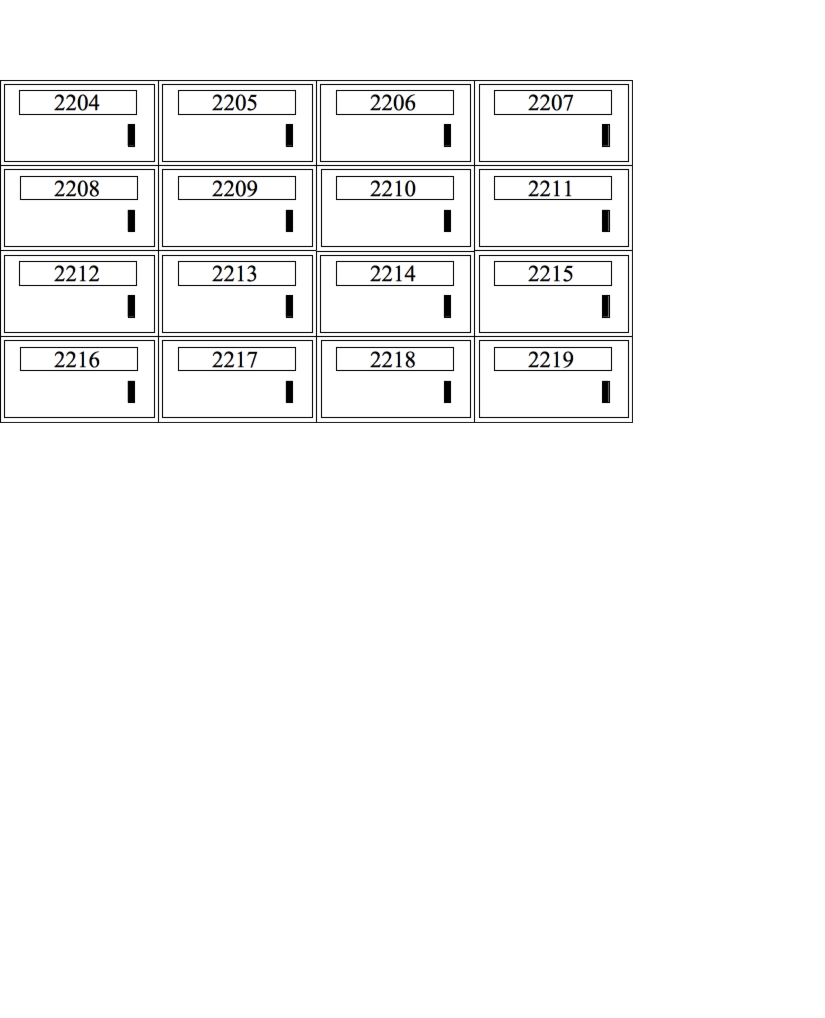
\includegraphics[width=\textwidth]{mailbox.png}
\end{figure}

You may wonder why a computer is organized this way.  It is because
it is simple to implement.  If the computer were composed of
a lot of differently-sized locations, or if you could store different
kinds of data in them, it would be difficult and expensive to
implement.

The computer's memory\index{memory} is used for a number of different things.  
All of the results of any calculations are stored in memory.  In fact,
everything that is "stored" is stored in memory.  Think of your computer
at home, and imagine what all is stored in your computer's memory.

\begin{itemize}\item The location of your cursor on the screen 
\item The size of each window on the screen 
\item The shape of each letter of each font being used 
\item The layout of all of the controls on each window 
\item The graphics for all of the toolbar icons 
\item The text for each error message and dialog box 
\item The list goes on and on... 
\end{itemize}

In addition to all of this, the Von Neumann architecture\index{Von Neumann architecture} specifies that
not only computer data should live in memory, but the programs that 
control the computer's operation should live there, too.  In fact, in 
a computer, there is no difference between a program and a program's
data except how it is used by the computer.  They are both stored and
accessed the same way.

\section{The CPU}

So how does the computer function?  Obviously, simply storing data doesn't
do much help - you need to be able to access, manipulate, and move it.  That's where
the CPU\index{CPU} comes in.

The CPU reads in instructions from memory one at a time and executes them.
This is known as the \emph{fetch-execute cycle}\index{fetch-execute cycle}.  The CPU
contains the following elements to accomplish this:

\begin{itemize}\item Program Counter\index{program counter} 
\item Instruction Decoder\index{instruction decoder} 
\item Data bus\index{data bus} 
\item General-purpose registers\index{general-purpose registers} 
\item Arithmetic and logic unit\index{arithmetic and logic unit} 
\end{itemize}

The \emph{program counter} is used to tell the computer where
to fetch the next instruction from.  We mentioned earlier that there is no
difference between the way data and programs are stored, they are just 
interpreted differently by the CPU.  The program counter holds the 
memory address of the next instruction
to be executed.  The CPU begins by looking at the program counter, and fetching
whatever number is stored in memory at the location specified.  It is then
passed on to the \emph{instruction decoder}\index{instruction decoder} which figures
out what the instruction means.  This includes what process needs to take
place (addition, subtraction, multiplication, data movement, etc.) and 
what memory locations are going to be involved in this process.  Computer
instructions usually consist of both the actual instruction and the list
of memory locations that are used to carry it out.

Now the computer uses the \emph{data bus}\index{data bus} to fetch the memory
locations to be used in the calculation.  The data bus is the connection
between the CPU and memory.  It is the actual wire that connects them.  If
you look at the motherboard of the computer, the wires that go out from the
memory are your data bus.

In addition to the memory on the outside of the processor, the processor
itself has some special, high-speed memory locations called registers\index{registers}.  
There are two kinds of registers - \emph{general registers} and 
\emph{special-purpose registers}.  
General-purpose registers\index{general-purpose registers} are where the main action happens.  Addition, 
subtraction, multiplication, comparisions, and other operations generally
use general-purpose registers for processing.  However, computers have very
few general-purpose registers.  Most information is stored in main memory,
brought in to the registers for processing, and then put back into memory
when the processing is completed.
\emph{special-purpose registers\index{special-purpose registers}} are registers which have very specific
purposes.  We will discuss these as we come to them.

Now that the CPU has retrieved all of the data it needs, it passes on
the data and the decoded instruction to the \emph{arithmetic and logic unit\index{arithmetic and logic unit}}
for further processing.  Here the instruction is actually executed.
After the results of the computation have been calculated, the results
are then placed on the data bus\index{data bus} and sent to the appropriate location
in memory or in a register, as specified by the instruction.

This is a very simplified explanation.  Processors have advanced quite
a bit in recent years, and are now much more complex. 
Although the basic operation is still
the same, it is complicated by the use of cache hierarchies\index{cache hierarchies}, superscalar
processors\index{superscalar
processors}, pipelining\index{pipelining}, branch prediction\index{branch prediction}, out-of-order execution\index{out-of-order execution}, 
microcode translation\index{microcode translation}, coprocessors\index{coprocessors}, and other optimizations.  Don't worry
if you don't know what those words mean, you can just use them as Internet search
terms if you want to learn more about the CPU.

\section{Some Terms}

Computer memory\index{computer memory} is a numbered sequence of fixed-size storage locations.  
The number attached to each storage location is called its 
\emph{address\index{address}}.  The size of a single storage location
is called a \emph{byte}.  On x86 processors, a byte\index{bytes} 
is a number between 0 and 255.  

You may be wondering how computers can display and use text, graphics,
and even large numbers when all they can do is store numbers between
0 and 255.  First of all, specialized hardware like graphics cards have special interpretations of
each number.  When displaying to the screen, the computer uses 
ASCII\index{ASCII} code tables to translate the numbers you are sending it
into letters to display on the screen, with each number translating to
exactly one letter or numeral.\footnote{With the advent of international
character sets and Unicode, this is not entirely true anymore.  However, for
the purposes of keeping this simple for beginners, we will use the assumption
that one number translates directly to one character.  For more information,
see \autoref{asciilisting}.}  For example, 
the capital letter A is 
represented by the number 65.   The numeral 1 is represented by the
number 49.  So, to print out "HELLO", you would actually give the
computer the sequence of numbers 72, 69, 76, 76, 79.  To print out
the number 100, you would give the computer the sequence of numbers
49, 48, 48.  A list of ASCII characters and their numeric codes
is found in \autoref{asciilisting}.

In addition to using numbers to represent ASCII characters, you as the 
programmer get to make the numbers mean anything you want them to, as well.  
For example, if I am running a store, I would use a number to represent 
each item I was selling.  Each number would be linked to a series of 
other numbers which would be the ASCII\index{ASCII} codes for what I wanted to display 
when the items were scanned in.  I would have more numbers for the price, 
how many I have in inventory, and so on.

So what about if we need numbers larger than 255?  We can simply use
a combination of bytes to represent larger numbers.  Two bytes can
be used to represent any number between 0 and 65535.  Four bytes
can be used to represent any number between 0 and 4294967295.  Now, it
is quite difficult to write programs to stick bytes together to increase
the size of your numbers, and requires a bit of math.  Luckily, the computer
will do it for us for numbers up to 4 bytes long.  In fact, four-byte numbers
are what we will work with by default.

We mentioned earlier that in addition to the regular memory that the 
computer has, it also has
special-purpose storage locations called \emph{registers\index{registers}}.
Registers are what the computer uses for computation.  
Think of a register as a place on your desk - it holds things you are currently
working on.  You may have lots of information tucked away in folders and
drawers, but the stuff you are working on right now is on the desk.  
Registers keep the contents of numbers that you are currently manipulating.

On the computers
we are using, registers are each four bytes long.  The size of a typical
register is called a computer's \emph{word\index{word}} size.  x86 processors have four-byte words.  This means that it is most natural on
these computers to do computations four bytes at a time.\footnote{Previous incarnations of x86 processors only had two-byte words.  Therefore,
most other literature dealing with x86 processors refers to two-byte entities
as words for historical reasons, and therefore refer to four-byte entities as 
double-words.  We are using the term \emph{word} to mean the 
normal register size of a computer, which in this case is four bytes.  More
information is available in \autoref{instructionsappendix},
}
  This gives us
roughly 4 billion values.

Addresses are also four bytes (1 word) long, and therefore also fit into a 
register.  x86 processors can access
up to 4294967296 bytes if enough memory is installed.  Notice that this
means that we can store addresses the same way we store any other number.
In fact, the computer can't tell the difference between a value that is
an address, a value that is a number, a value that is an ASCII code, or
a value that you have decided to use for another purpose.  A number becomes
an ASCII code when you attempt to display it.  A number becomes an address
when you try to look up the byte it points to.  Take a moment to think about
this, because it is crucial to understanding how computer programs work.

Addresses which are stored in memory are also called 
\emph{pointers\index{pointers}}, because instead of having a regular
value in them, they point you to a different location in memory.

As we've mentioned, computer instructions are also stored in memory.  
In fact, they are stored
exactly the same way that other data is stored.  The only way the computer
knows that a memory location is an instruction is that a special-purpose register\index{special-purpose register} called the instruction pointer\index{instruction pointer} points to them at one point or another.  If the instruction pointer points
to a memory word, it is loaded as an instruction.  Other than that, the 
computer has no way of knowing the difference between programs and other types
of data.\footnote{Note that here we are talking about general computer
theory.  Some processors and operating systems actually mark the regions
of memory that can be executed with a special marker that indicates this.
}

\section{Interpreting Memory}
\label{interpretingmemory}

Computers are very exact.  Because they are exact, programmers have to be
equally exact.  A computer has no idea what your program is supposed to
do.  Therefore, it will only do exactly what you tell it to do.  If you
accidentally print out a regular number instead of the ASCII codes that make up the number's digits, the
computer will let you - and you will wind up with jibberish on your screen (it will try to look up what your number represents in ASCII and print that).
If you tell the computer to start executing instructions at a location
containing data instead of program instructions, who knows how the computer will interpret that - 
but it will certainly try.  The computer will execute your instructions in
the exact order you specify, even if it doesn't make sense.

The point is, the computer will do exactly
what you tell it, no matter how little sense it makes.  Therefore, as
a programmer, you need to know exactly how you have your data arranged
in memory.  Remember, computers can only store numbers, so letters, pictures,
music, web pages, documents, and anything else are just long sequences
of numbers in the computer, which particular programs know how to interpret.

For example, say that you wanted to store customer information in memory.
One way to do so would be to set a maximum size for the customer's name 
and address - say 50 ASCII characters for each, which would be 50 bytes for each.
Then, after that, have a number for the customer's age and their customer
id.  In this case, you would have a block of memory that would look like
this:

\begin{simpletyping}
\begin{lstlisting}
Start of Record:
     Customer's name (50 bytes) - start of record
     Customer's address (50 bytes) - start of record + 50 bytes
     Customer's age (1 word = 4 bytes) - start of record + 100 bytes
     Customer's id number (1 word = 4 bytes) - start of record + 104 bytes
\end{lstlisting}
\end{simpletyping}

This way, given the address of a customer record, you know where the rest
of the data lies.  However, it does limit the customer's name and address
to only 50 ASCII characters each.

What if we didn't want to specify a limit?
Another way to do this would be to have in our record pointers\index{pointers} to this
information.  For example, instead of the customer's name, we would have
a pointer to their name.  In this case, the memory would look like this:

\begin{simpletyping}
\begin{lstlisting}
Start of Record:
     Customer's name pointer (1 word) - start of record
     Customer's address pointer (1 word) - start of record + 4
     Customer's age (1 word) - start of record + 8
     Customer's id number (1 word) - start of record + 12
\end{lstlisting}
\end{simpletyping}

The actual name and address would be stored elsewhere in memory.  This
way, it is easy to tell where each part of the data is from the start
of the record, without explicitly limitting the size of the name and
address.  If the length of the fields within our records could change,
we would have no idea where the next field started.  Because records
would be different sizes, it would also be hard to find where the
next record began.  Therefore, almost all records are of fixed lengths.
Variable-length data is usually stored separately from the rest of the
record.

\section{Data Accessing Methods}
\label{dataaccessingmethods}

%  FIXME - this would be a good section for diagrams 

Processors have a number of different ways of accessing data, known
as addressing modes\index{addressing modes}.  The simplest mode is 
\emph{immediate mode\index{immediate mode addressing}}, in which the data to access is
embedded in the instruction itself.  For example, if we want to initialize
a register to 0, instead of giving the computer an address to read the
0 from, we would specify immediate mode, and give it the number 0.

In the \emph{register addressing mode}\index{register addressing mode},
the instruction contains a register to access, rather than a memory location.
The rest of the modes will deal with addresses.

In the \emph{direct addressing mode\index{direct addressing mode}}, the instruction contains
the memory address to access.  For example, I could say, please load
this register with the data at address 2002.  The computer would go
directly to byte number 2002 and copy the contents into our register.

In the \emph{indexed addressing mode\index{indexed addressing mode}}, the instruction contains
a memory address to access, and also specifies an \emph{index register\index{index register}} to offset that address.  For example, we could specify
address 2002 and an index register.  If the index register contains the
number 4, the actual address the data is loaded from would be 2006.  This
way, if you have a set of numbers starting at location 2002, you can cycle
between each of them using an index register.  On x86 processors, you can
also specify a \emph{multiplier\index{multiplier}} for the index.  This allows you to access
memory a byte at a time or a word at a time (4 bytes).  If you are accessing
an entire word, your index will need to be multiplied by 4 to get the exact
location of the fourth element from your address.  For example, if you wanted
to access the fourth byte from location 2002, you would load your index
register with 3 (remember, we start counting at 0) and set the multiplier
to 1 since you are going a byte at a time.  This would get you location
2005.  However, if you wanted to access the fourth word from location 2002,
you would load your index register with 3 and set the multiplier to 4. 
This would load from location 2014 - the fourth word.  Take the time to 
calculate these yourself to make sure you understand how it works.

In the \emph{indirect addressing mode\index{indirect addressing mode}}, the instruction contains
a register that contains a pointer to where the data should be accessed.
For example, if we used indirect addressing mode and specified the {\eaxReg} 
register, and the {\eaxReg} register contained the value 4, whatever value was 
at memory location 4 would be used.  In direct addressing, we would just 
load the value 4, but in indirect addressing, we use 4 as the address to use 
to find the data we want.

Finally, there is the \emph{base pointer addressing mode\index{base pointer addressing mode}}.  This is
similar to indirect addressing, but you also include a number called the
\emph{offset\index{offset}} to add to the register's value before using it for lookup.  We will use this 
mode quite a bit in this book.

  
In \autoref{interpretingmemory} we discussed having a structure
in memory holding customer information.  Let's say we wanted to access
the customer's age, which was the eighth byte of the data, and we had the address 
of the start of the structure in a register.  We could use base pointer 
addressing and specify the register as the base pointer, and 8 as our offset.
This is a lot like indexed addressing, with the difference that the offset is
constant and the pointer is held in a register, and in indexed addressing
the offset is in a register and the pointer is constant.

There are other forms of addressing, but these are the most
important  ones.

\section{Review}

\section{Know the Concepts}

\begin{itemize}\item Describe the fetch-execute cycle. 
\item What is a register?  How would computation be more difficult without registers? 
\item How do you represent numbers larger than 255? 
\item How big are the registers on the machines we will be using? 
\item How does a computer know how to interpret a given byte or set of bytes of memory? 
\item What are the addressing modes and what are they used for? 
\item What does the instruction pointer do? 
\end{itemize}

\section{Use the Concepts}

\begin{itemize}\item What data would you use in an employee record?  How would you lay it out in memory? 
\item If I had the pointer to the beginning of the employee record above, and wanted to access a particular piece of data inside of it, what addressing mode would I use? 
\item In base pointer addressing mode, if you have a register holding the value 3122, and an offset of 20, what address would you be trying to access? 
\item In indexed addressing mode, if the base address is 6512, the index register has a 5, and the multiplier is 4, what address would you be trying to access? 
\item In indexed addressing mode, if the base address is 123472, the index register has a 0, and the multiplier is 4, what address would you be trying to access? 
\item In indexed addressing mode, if the base address is 9123478, the index register has a 20, and the multiplier is 1, what address would you be trying to access? 
\end{itemize}

\section{Going Further}

\begin{itemize}\item What are the minimum number of addressing modes needed for computation? 
\item Why include addressing modes that aren't strictly needed? 
\item Research and then describe how pipelining (or one of the other complicating factors) affects the fetch-execute cycle. 
\item Research and then describe the tradeoffs between fixed-length instructions and variable-length instructions. 
\end{itemize}


\chapter{Your First Programs}
\label{firstprogs}

% 
% 
% Copyright 2002 Jonathan Bartlett
% 
% Permission is granted to copy, distribute and/or modify this
% document under the terms of the GNU Free Documentation License,
% Version 1.1 or any later version published by the Free Software
% Foundation; with no Invariant Sections, with no Front-Cover Texts,
% and with no Back-Cover Texts.  A copy of the license is included in fdl.xml
% 

In this chapter you will learn the process for writing and building
Linux assembly-language programs.  In addition, you will learn the 
structure of assembly-language programs, and a few assembly-language
commands.  As you go through this chapter, you may want to refer also
to \autoref{instructionsappendix} and 
\autoref{gdbappendix}.

These programs may overwhelm you at first.  However, go through
them with diligence, read them and their explanations as many times
as necessary, and you will have a solid foundation of knowledge to
build on.  Please tinker around with the programs as much as you can.
Even if your tinkering does not work, every failure will help you learn.

\section{Entering in the Program}

Okay, this first program is simple.  In fact, it's not
going to do anything but exit!  It's short, but it shows
some basics about assembly language and Linux programming.
You need to enter the program in an editor exactly as written, 
with the filename \icodefilename{exit.s}.  The program follows.
Don't worry about not understanding it.  This section only deals with
typing it in and running it.  In \autoref{assemblyoutline} we
will describe how it works.

\begin{simpletyping}
\lstinputlisting{exit.s}
\end{simpletyping}

What you have typed in is called the \emph{source code\index{source code}}.
Source code is the human-readable form of a program.  In order to
transform it into a program that a computer can run, we need to 
\emph{assemble\index{assemble}} and \emph{link\index{link}} it.

The first step is to \emph{assemble} it.  Assembling is the
process that transforms what you typed into instructions for the machine.  
The machine itself only reads sets of numbers, but humans prefer words.
An \emph{assembly language\index{assembly language}} is a more human-readable
form of the instructions a computer understands.  Assembling transforms
the human-readable file into a machine-readable one.
To assembly the program type in the command

\begin{simpletyping}
\begin{lstlisting}
as exit.s -o exit.o
\end{lstlisting}
\end{simpletyping}

\icode{as}\index{\icode{as}} is the command which runs the assembler,  
\icodefilename{exit.s} is the source file\index{source file}, and 
\icode{-o exit.o} tells the assemble to put its output
in the file \icodefilename{exit.o}.
\icodefilename{exit.o} is an \emph{object file\index{object file}}.  An
object file is code that is in the machine's language, but has not
been completely put together.  In most large programs, you will have
several source files, and you will convert
each one into an object file.  The \emph{linker}\index{linker} is the program that is
responsible for putting the object files together and adding 
information to it so that the kernel knows how to load and run it.
In our case, we only have one object file, so the linker is only adding
the information to enable it to run.  To \emph{link\index{link}} the
file, enter the command

\begin{simpletyping}
\begin{lstlisting}
ld exit.o -o exit
\end{lstlisting}
\end{simpletyping}

\icode{ld}\index{ld} is the command to run the linker, 
\icodefilename{exit.o} is the object file we want to link,
and \icode{-o exit} instructs the linker to output
the new program into a file called \icodefilename{exit}.\footnote{If you are new to Linux and UNIX\textregistered, you may not be aware that files don't
have to have extensions.  In fact, while Windows\textregistered uses the 
\icode{.exe} extension to signify an executable program,
UNIX executables usually have no extension.}  If any
of these commands reported errors, you have either mistyped your program
or the command.  After
correcting the program, you have to re-run all the commands.
\emph{You must always re-assemble and re-link
programs after you modify the source file for the changes to occur in the
program}. You can run \icodefilename{exit} by typing in 
the command

\begin{simpletyping}
\begin{lstlisting}
./exit
\end{lstlisting}
\end{simpletyping}

The \icodefilename{./}\index{\icodefilename{./}} is used to tell the computer that the program
isn't in one of the normal program directories, but is the current
directory instead\footnote{\icodefilename{.} refers 
to the current directory in Linux and UNIX systems.}.  
You'll notice
when you type this command, the only thing that happens is that you'll go
to the next line.  That's because this program does nothing but exit.
However, immediately after you run the program, if you type in

\index{echo}
\index{\$?}

\begin{simpletyping}
\begin{lstlisting}
echo \$?
\end{lstlisting}
\end{simpletyping}

It will say \icode{0}.  What is happening is that every program
when it exits gives Linux an \emph{exit status code\index{exit status code}},
which tells it if everything went all right.  If everything was okay, it
returns 0.  UNIX programs return numbers other than zero to indicate 
failure or other errors, warnings, or statuses.  The programmer determines what each number means.  You can view this code by typing in 
\icode{echo \$?}.
In the following section we will look at what each part of the code
does.

\section{Outline of an Assembly Language Program}
\label{assemblyoutline}

Take a look at the program we just entered.  At the beginning there are
lots of lines that begin with
hashes (\icode{\#}).  These are \emph{comments\index{comments}}.
Comments are not translated by the assembler.  They are used only for
the programmer to talk to anyone who looks at the
code in the future.  Most programs you write will be modified by others.  Get 
into the habit of writing comments in your code that will
help them understand both why the program exists and how it works.  
Always include the following in your comments:

\begin{itemize}
\item The purpose of the code 
\item An overview of the processing involved 
%  FIXME - Dominique suggests an extended example of this 

\item Anything strange your program does and why it does 
it\footnote{You'll find that many programs end up doing things strange
ways.  Usually there is a reason for that, but, unfortunately, programmers
never document such things in their comments.  So, future programmers either
have to learn the reason the hard way by modifying the code and watching it
break, or just leaving it alone whether it is still needed or not.  You
should \emph{always} document any strange behavior your program
performs.  Unfortunately, figuring out what is strange and what is straightforward comes mostly with experience.} 
\end{itemize}

After the comments, the next line says

\begin{simpletyping}
\begin{lstlisting}
	.section .data
\end{lstlisting}
\end{simpletyping}

Anything starting with a period isn't directly translated into a machine 
instruction.  Instead, it's an instruction to the assembler itself.  These
are called \emph{assembler directives\index{assembler directives}} or \emph{pseudo-operations\index{pseudo-operations}} because they are handled by the assembler and are not actually run by the computer.
The \icode{.section}\index{\icode{.section}}
command breaks your program up into sections.  This command starts the
data section\index{data section}, 
where you list any memory storage you will need for data.  
Our program doesn't use any, so we don't need the section.  It's just here
for completeness.  Almost every program you write in the future will have data.

Right after this you have

\begin{simpletyping}
\begin{lstlisting}
	.section .text
\end{lstlisting}
\end{simpletyping}

\index{\icode{.text}}
which starts the text section.  The text 
section\index{text section} of a program 
is where the program instructions live.

The next instruction is

\begin{simpletyping}
\begin{lstlisting}
	.globl \_start
\end{lstlisting}
\end{simpletyping}

This instructs the assembler that \icode{\_start}\index{\icode{\_start}} is important
to remember.  \icode{\_start} is a \emph{symbol\index{symbol}},
which means that it is going to be replaced by something else either
during assembly or linking.  Symbols are generally used to mark locations
of programs or data, so you can refer to them by name instead of by their
location number.  Imagine if you had to refer to every memory location
by its address.  First of all, it would be very confusing because you would
have to memorize or look up the numeric memory address of every piece of code
or data.  In addition, every time you had to insert a piece of data or
code you would have to change all the addresses in your program!  
Symbols are used so that the assembler and linker can take care of
keeping track of addresses, and you can concentrate on writing your
program.

\icode{.globl}\index{\icode{.globl}} means that the assembler shouldn't
discard this symbol after assembly, because the linker will need it.  
\icode{\_start}\index{\icode{\_start}} is a special symbol that always needs to be 
marked with \icode{.globl} because it marks the location of the
start of the program.  \emph{Without marking this 
location in this way, when the computer loads your program it won't know 
where to begin running your program}.

The next line

\begin{simpletyping}
\begin{lstlisting}
\_start:
\end{lstlisting}
\end{simpletyping}

\emph{defines} the value of the \icode{\_start}\index{\_start} label. A \emph{label\index{labels}} 
is a symbol\index{symbol} followed by
a colon.  Labels define a symbol's value.  When the 
assembler\index{assembler} is assembling
the program, it has to assign each data value and instruction an address.
Labels tell the assembler to make the symbol's value be wherever the
next instruction or data element will be.  This way, if the actual
physical location of the data or instruction changes, you don't have to
rewrite any references to it - the symbol automatically gets the new value.

Now we get into actual computer instructions.  The first such instruction is this:

\begin{simpletyping}
\begin{lstlisting}
movl \$1, {\eaxBare}
\end{lstlisting}
\end{simpletyping}

When the program runs, this instruction transfers 
the number \icode{1} into the {\eaxReg} register.  In assembly language,
many instructions have \emph{operands}\index{operands}.  \icode{movl}\index{movl} has two operands - 
the \emph{source} and the \emph{destination}.  In
this case, the source is the literal number 1, and the destination is the
{\eaxReg} register.  Operands can be numbers, memory location references, or
registers.  Different instructions allow different types of operands.  See
\autoref{instructionsappendix} for more information on which 
instructions take which kinds of operands.

On most instructions which
have two operands, the first one is the source operand and the second one
is the destination.  Note that in these cases, the source operand is not
modified at all.  Other instructions of this type are, for example,
\icode{addl}\index{addl}, 
\icode{subl}\index{subl}, and  
\icode{imull}\index{imull}.
These add/subtract/multiply
the source operand from/to/by the destination operand and and save the result
in the destination operand.  Other instructions may have an operand hardcoded
in.  \icode{idivl}\index{idivl}, 
for example, requires that the dividend be
in {\eaxReg}, and {\edxReg} be zero, and the quotient is then transferred to {\eaxReg}
and the remainder to {\edxReg}.  However, the divisor can be any register or 
memory location.

On x86 processors, there are several general-purpose registers\index{general-purpose registers}\footnote{Note that on x86 processors, even the general-purpose registers have some special purposes, or used to before it went 32-bit.  However, these are general-purpose registers for most instructions.  Each of them has at least one instruction where it is used in a special way.  However, for most of them, those instructions aren't covered in this book.}
 (all of which can be used with \icode{movl}):

\begin{itemize}\item {\eaxRegIdx} 
\item {\ebxRegIdx} 
\item {\ecxRegIdx} 
\item {\edxRegIdx} 
\item {\ediRegIdx} 
\item {\esiRegIdx} 
\end{itemize}

In addition to these general-purpose registers,
there are also several special-purpose registers\index{special-purpose registers}, including:

\begin{itemize}\item {\ebpRegIdx} 
\item {\espRegIdx} 
\item {\eipRegIdx} 
\item {\eflagsRegIdx} 
\end{itemize}

We'll discuss these later, just be aware that they 
exist.\footnote{You may be wondering, \emph{why do all of these
registers begin with the letter \icode{e}?}  The
reason is that early generations of x86 processors were 16 bits 
rather than 32 bits.
Therefore, the registers were only half the length
they are now.  In later generations of x86 processors, the size of the 
registers doubled. They kept
the old names to refer to the first half of the register, and added an
\icode{e} to refer to the extended versions of the register.
Usually you will only use the extended versions.  Newer models also
offer a 64-bit mode, which doubles the size of these registers yet again
and uses an \icode{r} prefix to indicate the larger registers (i.e.
{\raxReg} is the 64-bit version of {\eaxReg}).  However, these processors are not 
widely used, and are not covered in this book.
}  Some of these registers, like {\eipRegIdx} and {\eflagsRegIdx} can
only be accessed through special instructions.  The others can be accessed
using the same instructions as general-purpose registers, but they have 
special meanings, special uses, or are simply faster when used in a specific
way.

So, the \icode{movl}\index{\icode{movl}} instruction moves the number 
\icode{1} into \icode{{\eaxBare}}.  The 
dollar-sign in front of the one indicates that we want to use 
immediate mode addressing\index{immediate mode addressing} (refer back to \autoref{dataaccessingmethods}).  Without the dollar-sign it would do direct addressing\index{direct addressing mode},
loading whatever number is at address \icode{1}.  We want the
actual number \icode{1} loaded in, so we have to use immediate
mode.  

The reason we are moving the number 1 into {\eaxReg} is because we are 
preparing to call the Linux Kernel. The
number \icode{1} is the number of the \icode{exit}\index{\icode{exit}}
\emph{system call}
\index{system call}.
We will discuss system calls in more depth soon, but basically they are 
requests for the operating system's help.  Normal programs can't do 
everything.  Many operations such as calling other programs, dealing with 
files, and exiting have to be handled
by the operating system through system calls\index{system calls}.
When you make a system call, which we will do shortly, the system
call number has to be loaded into {\eaxRegIdx}
(for a complete listing of system calls and their numbers,
see \autoref{syscallap}).
Depending on the system call, other registers may have
to have values in them as well.  Note that system calls is not the only use or
even the main use of registers.  It is just the one we are dealing with in
this first program.  Later programs will use registers for regular 
computation.

The operating system, however, usually needs more information than just which
call to make.   For example, when dealing with files, the operating system 
needs to know which file you are dealing with, what data you want to write, 
and other
details.  The extra details, called \emph{parameters\index{parameters}}
are stored in other registers.  In the case of the \icode{exit} system call,
the operating system requires a status code be loaded in {\ebxRegIdx}.  This 
value is then returned to the system.  This is the value you retrieved 
when you typed \icode{echo \$?}.  So, we load {\ebxReg} with 
\icode{0} by typing the following:

\begin{simpletyping}
\begin{lstlisting}
movl \$0, {\ebxBare}
\end{lstlisting}
\end{simpletyping}

Now, loading 
registers\index{registers} with these 
numbers doesn't do anything itself.
Registers are used for all sorts of things besides system calls.  They
are where all program logic such as addition, subtraction, and comparisons
take place.  Linux simply requires that certain registers be loaded with
certain parameter values before making a system call.  {\eaxRegIdx} is 
always required to be loaded with the system call number.  
For the other registers, however, each system call has different requirements.
In the \icode{exit\index{exit}}
system call, {\ebxRegIdx} is required to be loaded with the exit status\index{exit status code}.
We will discuss different system calls as they are needed.  For a list of
common system calls and what is required to be in each register, see \autoref{syscallap}

The next instruction is the "magic" one.  It looks like this:

\begin{simpletyping}
\begin{lstlisting}
	int \$0x80
\end{lstlisting}
\end{simpletyping}

The \icode{int\index{int}} stands for 
\emph{interrupt\index{interrupts}}.  The
\icode{0x80\index{0x80}} is the interrupt 
number to use.\footnote{You
may be wondering why it's \icode{0x80} instead of just 
\icode{80}.  The reason is that the number is written in 
hexadecimal\index{hexadecimal}.  In hexadecimal, a single digit can hold 16 values instead
of the normal 10.  This is done by utilizing the letters 
\icode{a} through \icode{f}
in addition to the regular digits.  \icode{a} represents 10,
\icode{b} represents 11, and so on.  0x10 represents the number
16, and so on.  This will be discussed more in depth later, but just be
aware that numbers starting with \icode{0x} are in hexadecimal.
Tacking on an \icode{H} at the end is also sometimes used instead, but
we won't do that in this book.  For more information about this, see \autoref{countingchapter}
}

An \emph{interrupt\index{interrupts}} interrupts the normal program flow, and
transfers control from our program to Linux\index{Linux} so that it will do a system
call.\footnote{Actually, the
interrupt transfers control to whoever set up an \emph{interrupt
handler} for the interrupt number.  In the case of Linux,
all of them are set to be handled by the Linux kernel.}.
You can think of it as like signaling Batman(or 
Larry-Boy\index{Larry-Boy}\footnote{If you don't watch Veggie Tales, you should.  Start with Dave and the Giant Pickle.}, if you prefer).
You need something done,
you send the signal, and then he comes to the rescue.  You don't care how
he does his work - it's more or less magic - and when he's done you're
back in control.  In this case, all we're doing is asking Linux to 
terminate the program, in which case we won't be back in control.  
If we didn't signal the interrupt, then no system call would have been
performed.

\begin{sidebar}[Quick System Call Review]
To recap - Operating System features are accessed through
system calls\index{system calls}.  These are invoked by setting up the registers
in a special way and issuing the instruction \icode{int \$0x80}.
Linux knows which system call we want to access by what we stored
in the {\eaxRegIdx} register.  Each system call has other requirements
as to what needs to be stored in the other registers.  System call
number 1 is the \icode{exit} system call, which requires
the status code\index{status code}
to be placed in {\ebxRegIdx}.
\end{sidebar}

Now that you've assembled, linked, run, and examined the program, you
should make some basic edits.  Do things like change the number 
that is loaded into \icode{{\ebxBare}}, and watch it come out
at the end with \icode{echo \$?\index{echo}\index{\$?}}.  Don't forget
to assemble and link it again before running it.
Add some comments.  Don't worry, the worse thing that would happen is that the 
program won't assemble or link, or will freeze your screen.  That's just
part of learning!

\section{Planning the Program}

In our next program we will try to find the maximum of a list of numbers.
Computers are very detail-oriented, so in order to write the program we
will have to have planned out a number of details.  These details include:

\begin{itemize}\item Where will the original list of numbers be stored? 
\item What procedure will we need to follow to find the maximum number? 
\item How much storage do we need to carry out that procedure? 
\item Will all of the storage fit into registers, or do we need to use some memory as well? 
\end{itemize}

You might not think that something as simple as finding the maximum number from
a list would take much planning.  You can usually tell people to find the 
maximum number, and they can do so with little trouble.  However, our minds
are used to putting together complex tasks automatically.  Computers need
to be instructed through the process.  In addition, we can usually hold any
number of things in our mind without much trouble.  We usually don't even
realize we are doing it.  For example, if you scan a list of numbers for the
maximum, you will probably keep in mind both the highest number you've seen
so far, and where you are in the list.  While your mind does this
automatically, with computers you have to explicitly set up storage for holding
the current position on the list and the current maximum number.  You also
have other problems such as how to know when to stop.  When reading a piece
of paper, you can stop when you run out of numbers.  However, the computer
only contains numbers, so it has no idea when it has reached the last of 
\emph{your} numbers.

In computers, you have to plan every step of the way.  So, let's do
a little planning.  First of all, just for reference, let's name the
address where the list of numbers starts as \icode{data\_items}.
Let's say that the last number in the list will be a zero, so we know where
to stop.  We also need a value to hold the current position in the list,
a value to hold the current list element being examined, and the current
highest value on the list.  Let's assign each of these a register:

\begin{itemize}\item {\ediReg} will hold the current position in the list. 
\item {\ebxReg} will hold the current highest value in the list. 
\item {\eaxReg} will hold the current element being examined. 
\end{itemize}

When we begin the program and look at the first item in the list, since we
haven't seen any other items, that item will automatically be the current
largest element in the list.  Also, we will set the current position in the
list to be zero - the first element.  From then, we will follow the following
steps:

\begin{enumerate}\item Check the current list element ({\eaxReg}) to see if it's zero (the terminating element). 
\item If it is zero, exit. 
\item Increase the current position ({\ediReg}). 
\item Load the next value in the list into the current value register ({\eaxReg}).  What addressing mode might we use here?  Why? 
\item Compare the current value ({\eaxReg}) with the current highest value ({\ebxReg}). 
\item If the current value is greater than the current highest value, replace the current highest value with the current value. 
\item Repeat. 
\end{enumerate}

That is the procedure.  Many times in that procedure I made use of the word
"if".  These places are where decisions are to be made.  You see, the computer
doesn't follow the exact same sequence of instructions every time.  Depending
on which "if"s are correct, the computer may follow a different set of 
instructions.  The second time through, it might not have the highest value.
In that case, it will skip step 6, but come back to step 7.  In every 
case except the last one, it will skip step 2.  In more complicated programs,
the skipping around increases dramatically.

These "if"s are a class of instructions called \emph{flow control\index{flow control}} instructions, because they tell the computer which steps
to follow and which paths to take.  In the previous program, we did not
have any flow control instructions, as there was only one possible path to
take - exit.  This program is much more dynamic in that it is directed by
data.  Depending on what data it receives, it will follow different instruction
paths.

In this program, this will be accomplished by two different 
instructions, the conditional 
jump\index{conditional jump} and the 
unconditional jump\index{unconditional jump}.
The conditional
jump changes paths based on the results of a previous comparison or
calculation.  The unconditional jump just goes directly to a different path
no matter what.  The unconditional jump may seem useless, but it is very
necessary since all of the instructions will be laid out on a line.  If a
path needs to converge back to the main path, it will have to do this by
an unconditional jump.  We will see more of both of these jumps in the
next section.

Another use of flow control\index{flow control} is in implementing loops\index{loops}.  A loop is a piece
of program code that is meant to be repeated.  In our example, the first
part of the program (setting the current position to 0 and loading the
current highest value with the current value) was only done once, so it
wasn't a loop.  However, the next part is repeated over and over again
for every number in the list.  It is only left when we have come to the
last element, indicated by a zero.  This is called a \emph{loop}
because it occurs over and over again.  It is implemented by doing 
unconditional jumps to the beginning of the loop at the end of the loop, which
causes it to start over.  However, you have to always remember to have a
conditional jump to exit the loop somewhere, or the loop will continue
forever!  This condition is called an \emph{infinite loop\index{infinite loop}}.
If we accidentally left out step 1, 2, or 3, the loop (and our program)
would never end.

In the next section, we will implement this program that we have planned.
Program planning sounds complicated - and it is, to some degree.  When you
first start programming, it's often hard to convert our normal thought
process into a procedure that the computer can understand.  We often forget
the number of "temporary storage locations" that our minds are using to
process problems.  As you read and write programs, however, this will
eventually become very natural to you.  Just have patience.

\section{Finding a Maximum Value}
\label{maximum}

Enter the following program as \icodefilename{maximum.s}:

\begin{simpletyping}
\lstinputlisting{maximum.s}
\end{simpletyping}

Now, assemble and link it with these commands:

\begin{simpletyping}
\begin{lstlisting}
as maximum.s -o maximum.o
ld maximum.o -o maximum
\end{lstlisting}
\end{simpletyping}

Now run it, and check its status.

\begin{simpletyping}
\begin{lstlisting}
./maximum
echo \$?
\end{lstlisting}
\end{simpletyping}

You'll notice it returns the value \icode{222}.  Let's take
a look at the program and what it does.  If you look in the comments, you'll
see that the program finds the maximum of a set of numbers (aren't comments
wonderful!).  You may also notice that in this program we actually have 
something in the data section\index{data section}.  
These lines are the data section:

\begin{simpletyping}
\begin{lstlisting}
data\_items:                       \#These are the data items
        .long 3,67,34,222,45,75,54,34,44,33,22,11,66,0
\end{lstlisting}
\end{simpletyping}

Lets look at this.  \icode{data\_items} is a 
label\index{labels} that
refers to the location that follows it.  Then, there is a directive
that starts with \icode{.long\index{.long}}.  That causes the assembler
to reserve memory for the list of numbers that follow it.  
\icode{data\_items} refers to the location of the first one.  
Because \icode{data\_items} is a label, any time in our program
where we need to refer to this address we can use the 
\icode{data\_items} symbol, and the assembler will substitute
it with the address where the numbers start during assembly.  For example,
the instruction \icode{movl data\_items, {\eaxBare}} would move the
value 3 into {\eaxReg}.
There are several different types of memory locations other than \icode{.long\index{.long}}
that can be reserved.  The main ones are as follows:

\begin{description}
\item[\icode{.byte\index{.byte}}] Bytes take up one storage location for each number.  They are limited
to numbers between 0 and 255.
\item[\icode{.int\index{.int}}] Ints (which differ from the \icode{int} instruction) take up
two storage locations for each number.  These are limitted to numbers
between 0 and 65535.\footnote{Note that no numbers in assembly language
(or any other computer language I've seen) have commas embedded in them.  So,
always write numbers like \icode{65535}, and never like 
\icode{65,535}.}
\item[\icode{.long\index{.long}}] Longs take up four storage locations.  This is the same amount of 
space the registers use, which is why they are used in this program.
They can hold numbers between 0 and 4294967295.
\item[\icode{.ascii\index{.ascii}}] The \icode{.ascii} directive is to enter in characters
into memory.  Characters each take up one storage location (they are
converted into bytes internally).  So, if you gave the directive
\icode{.ascii "Hello there\\0"}, the assembler would reserve 12 storage
locations (bytes).  The first byte contains the numeric code for 
\icode{H}, the second byte contains the numeric code for
\icode{e}, and so forth.  The last character is represented
by \icode{\\0}\index{\\0}, 
and it is the terminating character (it will 
never display, it just tells other parts of the program that that's the
end of the characters).  Letters and numbers that start with a backslash
represent characters that are not typeable on the keyboard or easily viewable
on the screen.  
For example, \icode{\\n}\index{\\n} refers to the "newline"\index{newline} character which causes the computer to start output on the next line and \icode{\\t}
\index{\\t} refers to the "tab"\index{tab} character.  All of the letters in an \icode{.ascii} directive should be in quotes.
\end{description}

In our example, the assembler reserves 14 \icode{.long}s,
one right after another.  Since each long takes up 4 bytes, that means
that the whole list takes up 56 bytes.  These are the numbers we will
be searching through to find the maximum.  \icode{data\_items}
is used by the assembler to refer to the address of the first of these values.

Take note that the last data item in the list is a zero.  I decided 
to use a zero to tell my program that
it has hit the end of the list.  I could have done this other ways.  I
could have had the size of the list hard-coded into the program.  Also,
I could have put the length of the list as the first item, or in a separate
location.  I also could have made a symbol which marked the last location
of the list items.  No matter how I do it, I must have some method of 
determining the end of the list.  The computer knows nothing -
it can only do what it is told.  It's not going to stop processing unless I give
it some sort of signal.  Otherwise it would continue processing past the end
of the list into the data that follows it, and even to locations where 
we haven't put any data.

Notice that we don't have a 
\icode{.globl\index{.globl}} declaration for \icode{data\_items}.
This is because we only refer to these locations within the program.  No
other file or program needs to know where they are located.  This is
in contrast to the \icode{\_start\index{\_start}} symbol, which Linux
needs to know where it is so that it knows where to begin
the program's execution.  It's not an error to write 
\icode{.globl data\_items}, it's just not necessary.
Anyway, play around with this line and add your own numbers.  Even
though they are \icode{.long}, the program will produce
strange results if any number is greater than 255, because that's the
largest allowed 
exit status\index{exit status code}.  
Also notice that if you move the 0 to
earlier in the list, the rest get ignored.  
\emph{Remember that any time
you change the source file, you have to re-assemble and re-link
your program.  Do this now and see the results}.

All right, we've played with the data a little bit.  Now let's look
at the code.  In the comments you will notice that we've marked
some \emph{variables\index{variables}} 
that we plan to use.  A variable
is a dedicated storage location used for a specific purpose, usually
given a distinct name by the programmer.  We talked about these in the
previous section, but didn't give them a name.  In this program, we have 
several variables:

\begin{itemize}\item a variable for the current maximum number found 
\item a variable for which number of the list we are currently examining, called the index 
\item a variable holding the current number being examined 
\end{itemize}

In this case,we have few enough variables that we can hold them all in 
registers.  In larger programs, you have to put them in memory, and then move
them to registers\index{registers} when you are ready to use them.  We will discuss how 
to do that later.  When people start out programming, they usually 
underestimate the number of variables they will need.  People are not used 
to having to think through every detail of a process, and therefore leave out
needed variables in their first programming attempts.

In this program, we are using {\ebxReg} as the location 
of the largest item we've found.  {\ediReg} is used as the 
\emph{index\index{index}} to the current data item we're looking at.  
Now, let's talk about what an index is.  When we read the information 
from \icode{data\_items},
we will start with the first one (data item number 0), then go to the second
one (data item number 1), then the third (data item number 2), and so on.  
The data item number is the \emph{index\index{index}} of 
\icode{data\_items}.  You'll notice that the first instruction
we give to the computer is:

\begin{simpletyping}
\begin{lstlisting}
	movl \$0, {\ediBare}
\end{lstlisting}
\end{simpletyping}

Since we are using \icode{{\ediBare}} as our index, and we want to start
looking at the first item, we load \icode{{\ediBare}} with 0.  Now,
the next instruction is tricky, but crucial to what we're doing.  It says:

\begin{simpletyping}
\begin{lstlisting}
	movl data\_items(,{\ediBare},4), {\eaxBare}
\end{lstlisting}
\end{simpletyping}

\index{movl}

Now to understand this line, you need to keep several things in mind:

\begin{itemize}\item \icode{data\_items} is the location number of the start of our number list. 
\item Each number is stored across 4 storage locations (because we declared it using \icode{.long}) 
\item \icode{{\ediBare}} is holding 0 at this point 
\end{itemize}

So, basically what this line does is say, "start at the beginning of 
data\_items, and take the first item number (because \icode{{\ediBare}} 
is 0), and remember that each number takes up four storage locations."
Then it stores that number in \icode{{\eaxBare}}.  This is how you write
indexed addressing mode\index{indexed addressing mode}
instructions in assembly language.  The instruction in a general form
is this: 

\begin{simpletyping}
\begin{lstlisting}
movl  BEGINNINGADDRESS(,\%INDEXREGISTER,WORDSIZE)
\end{lstlisting}
\end{simpletyping}
  

In our case \icode{data\_items} was our beginning address, {\ediReg} was our
index register\index{index register}, and 4 was our word size.  This topic is discussed further in \autoref{movaddrmodes}.

If you look at the numbers in \icode{data\_items}, you will see that the number
3 is now in {\eaxReg}.  If {\ediReg} was set 
to 1, the number 67 would be in {\eaxReg}, and if it
was set to 2, the number 34 would be in {\eaxReg}, and so
forth.  Very strange things would happen if we used a number other than
4 as the size of our storage locations.\footnote{The instruction 
doesn't really use 4 for the size of the storage locations, although 
looking at it that way works for our purposes now.  It's actually what's 
called a \emph{multiplier\index{multiplier}}.  basically, the way it works is that
you start at the location specified by \icode{data\_items}, then
you add \icode{{\ediBare}}*4 storage locations, and retrieve the number
there.  Usually, you use the size of the numbers as your multiplier, but in
some circumstances you'll want to do other things.}
The way you write this is very awkward, but if you know what each piece does, 
it's not too difficult.  For more information about this, see 
\autoref{movaddrmodes}

Let's look at the next line:

\begin{simpletyping}
\begin{lstlisting}
	movl {\eaxBare}, {\ebxBare}
\end{lstlisting}
\end{simpletyping}

We have the first item to look at stored in \icode{{\eaxBare}}.  Since
it is the first item, we know it's the biggest one we've looked at.  
We store it in \icode{{\ebxBare}}, since that's where we are
keeping the largest number found.  Also, even though \icode{movl\index{movl}}
stands for \emph{move}, it actually copies the value, so
\icode{{\eaxBare}} and \icode{{\ebxBare}} both contain the
starting value.\footnote{Also, the \icode{l} in 
\icode{movl\index{movl}} stands for \emph{move long} since
we are moving a value that takes up four storage locations.}

Now we move into a \emph{loop\index{loop}}.  
A loop is a segment of your program that might run more than once.  We have marked the starting
location of the loop in the symbol \icode{start\_loop}.  The
reason we are doing a loop is because we don't know how many
data items we have to process, but the procedure will be the same no
matter how many there are.  We don't want to have to rewrite our program for 
every list length possible.  In fact, we don't even want to have to write out
code for a comparison for every list item.  Therefore, we have a single 
section of code (a loop) that we execute over and over again for every 
element in \icode{data\_items}.

In the previous section, we outlined what this loop needed to do.  Let's
review:

\begin{itemize}\item Check to see if the current value being looked at is zero.  If so, that means we are at the end of our data and should exit the loop. 
\item We have to load the next value of our list. 
\item We have to see if the next value is bigger than our current biggest value. 
\item If it is, we have to copy it to the location we are holding the largest value in. 
\item Now we need to go back to the beginning of the loop. 
\end{itemize}

Okay, so now lets go to the code.  We have the beginning of the loop 
marked with \icode{start\_loop}.  That is so we know where to go back
to at the end of our loop.  Then we have these instructions:

\begin{simpletyping}
\begin{lstlisting}
	cmpl \$0, {\eaxBare}
	je loop\_exit
\end{lstlisting}
\end{simpletyping}

The \icode{cmpl\index{cmpl}} instruction compares the two values.  Here,
we are comparing the number 0 to the number stored in {\eaxReg}
This compare instruction also affects a register not mentioned here, the
{\eflagsRegIdx} register.  This is also known as the status register\index{status register},
and has many uses which we will discuss later.  Just be aware that the
result of the comparison is stored in the status register.  The next line
is a flow control\index{flow control} instruction which says to 
\emph{jump} to the \icode{loop\_exit} location
if the values that were just compared are equal (that's what the 
\icode{e}
of \icode{je} means).  It uses the status register to hold the 
value of
the last comparison.  We used \icode{je}, but there are many jump 
statements that you can use:

\begin{description}
\item[\icode{je}] Jump if the values were equal
\item[\icode{jg}] Jump if the second value was greater than the first 
value\footnote{notice that the comparison is to see if the
\emph{second} value is greater than the first.  I
would have thought it the other way around.  You will find a lot of
things like this when learning programming.  It occurs because different
things make sense to different people.  Anyway, you'll just have to
memorize such things and go on.}
\item[\icode{jge}] Jump if the second value was greater than or equal to the first value
\item[\icode{jl}] Jump if the second value was less than the first value
\item[\icode{jle}] Jump if the second value was less than or equal to the first value
\item[\icode{jmp}] Jump no matter what.  This does not need to be preceeded by a 
comparison.
\end{description}

The complete list is documented in \autoref{instructionsappendix}.
In this case, we are jumping if {\eaxReg} holds the value
of zero.  If so, we are done and we go to 
\icode{loop\_exit}.\footnote{The names of these symbols
can be anything you want them to be, as long as they only contain letters
and the underscore character(\icode{\_}).  The only one that
is forced is \icode{\_start\index{\_start}}, and possibly others that you
declare with \icode{.globl\index{.globl}}.  However, if it is a symbol you
define and only you use, feel free to call it anything you want that is 
adequately descriptive (remember that others will have to modify your code 
later, and will have to figure out what your symbols mean).
}

If the last loaded element was not zero, we go on to the next instructions:

\begin{simpletyping}
\begin{lstlisting}
	incl {\ediBare}
	movl data\_items(,{\ediBare},4), {\eaxBare}
\end{lstlisting}
\end{simpletyping}

If you remember from our previous discussion, {\ediReg} contains
the index\index{index} to 
our list of values in \icode{data\_items}.
\icode{incl\index{incl}} 
increments the value of {\ediReg} by
one.  Then the \icode{movl} is just like the one we did 
beforehand.  However, since we already incremented {\ediReg}, {\eaxReg} is getting the
next value from the list.  Now {\eaxReg} has the next value to be tested.  
So, let's test it!

\begin{simpletyping}
\begin{lstlisting}
	cmpl {\ebxBare}, {\eaxBare}
	jle start\_loop
\end{lstlisting}
\end{simpletyping}

Here we compare our current value, stored in {\eaxReg}
to our biggest value so far, stored in {\ebxReg}.  If
the current value is less or equal to our biggest value so far, we don't 
care about it, so we just jump back to the beginning of the loop.  
Otherwise, we need to record that value as the largest one:

\begin{simpletyping}
\begin{lstlisting}
	movl {\eaxBare}, {\ebxBare}
	jmp start\_loop
\end{lstlisting}
\end{simpletyping}

which moves the current value into {\ebxReg}, which we are
using to store the current largest value,  and starts
the loop over again.  

Okay, so the loop executes until it reaches a 0, when it jumps
to \icode{loop\_exit}.  This part of the program calls
the Linux kernel to exit.  If you remember from the last program,
when you call the operating system (remember it's like signaling Batman), 
you store the 
system call\index{system call} 
number in {\eaxRegIdx} 
(1 for the \icode{exit} call),
and store the other values in the other registers.  The exit call
requires that we put our exit status\index{exit status code} in {\ebxRegIdx}
We already have the exit status there since we are using {\ebxReg}
as our largest number, so all we have to do is load {\eaxReg} with the number one
and call the kernel to exit. Like this:

\begin{simpletyping}
\begin{lstlisting}
	movl \$1, {\eaxBare}
	int  \$0x80
\end{lstlisting}
\end{simpletyping}

Okay, that was a lot of work and explanation, especially for such a
small program.  But hey, you're learning a lot!  Now,
read through the whole program again, paying special
attention to the comments.  Make sure that you understand what is going
on at each line.  If you don't understand a line, go back through this
section and figure out what the line means.

You might also grab a piece
of paper, and go through the program step-by-step, recording every change
to every register, so you can see more clearly what is going on.

\section{Addressing Modes}
\label{movaddrmodes}

In \autoref{dataaccessingmethods} we learned the different types
of addressing modes\index{addressing modes} available for use in assembly language.  This section
will deal with how those addressing modes are represented in assembly
language instructions.

The general form of memory address\index{memory address} references is this:

\begin{simpletyping}
\begin{lstlisting}
ADDRESS\_OR\_OFFSET(\%BASE\_OR\_OFFSET,\%INDEX,MULTIPLIER)
\end{lstlisting}
\end{simpletyping}

All of the fields are optional.  To calculate the address, simply perform
the following calculation:

\begin{simpletyping}
\begin{lstlisting}
FINAL ADDRESS = ADDRESS\_OR\_OFFSET + \%BASE\_OR\_OFFSET + MULTIPLIER * \%INDEX
\end{lstlisting}
\end{simpletyping}

\icode{ADDRESS\_OR\_OFFSET} and \icode{MULTIPLIER} must
both be constants, while the other two must be registers.  If any of the
pieces is left out, it is just substituted with zero in the equation.

All of the addressing modes mentioned in \autoref{dataaccessingmethods} except immediate-mode can be represented in this fashion.

\begin{description}
\item[direct addressing mode\index{direct addressing mode}] This is done by only using the \icode{ADDRESS\_OR\_OFFSET} portion.  Example:
\begin{simpletyping}
\begin{lstlisting}
movl ADDRESS, {\eaxBare}
\end{lstlisting}
\end{simpletyping}

This loads {\eaxReg} with the value at memory address \icode{ADDRESS}.
\item[indexed addressing mode\index{indexed addressing mode}] This is done by using the \icode{ADDRESS\_OR\_OFFSET} and the
\icode{\%INDEX} portion.  You can use any general-purpose
register as the index register.  You can also have a constant
multiplier\index{multiplier} of 1, 2, or 4 for the index register\index{index register}, to make it easier to
index by bytes, double-bytes, and words.  For example, let's say that
we had a string of bytes as \icode{string\_start} and wanted
to access the third one (an index of 2 since we start counting the
index at zero), and {\ecxReg} held the value 2.  If you wanted to load it
into {\eaxReg} you could do the following:
\begin{simpletyping}
\begin{lstlisting}
movl string\_start(,{\ecxBare},1), {\eaxBare}
\end{lstlisting}
\end{simpletyping}

This starts at \icode{string\_start}, and adds \icode{1 * {\ecxBare}} to that address, and loads the value into {\eaxReg}.
\item[indirect addressing mode\index{indirect addressing mode}] Indirect addressing mode loads a value from the address indicated by a register.  For example, if {\eaxReg} held an address, we could move the value at that
address to {\ebxReg} by doing the following:
\begin{simpletyping}
\begin{lstlisting}
movl ({\eaxBare}), {\ebxBare}
\end{lstlisting}
\end{simpletyping}
\item[base pointer addressing mode\index{base pointer addressing mode}] Base-pointer addressing is similar to indirect addressing, except that it
adds a constant value to the address in the register.  For example, if you
have a record where the age value is 4 bytes into the record, and you have the
address of the record in {\eaxReg}, you can retrieve the age into {\ebxReg} by 
issuing the following instruction:
\begin{simpletyping}
\begin{lstlisting}
movl  4({\eaxBare}), {\ebxBare}
\end{lstlisting}
\end{simpletyping}
\item[immediate mode\index{immediate mode addressing}] Immediate mode is very simple.  It does not follow the general form we have
been using.  Immediate mode is used to load direct values into registers
or memory locations.  For example, if you wanted to load the number 12
into {\eaxReg}, you would simply do the following:
\begin{simpletyping}
\begin{lstlisting}
movl \$12, {\eaxBare}
\end{lstlisting}
\end{simpletyping}

Notice that to indicate immediate mode, we used a dollar sign in front of
the number.  If we did not, it would be direct addressing mode, in which 
case the value located at memory location 12 would be loaded into {\eaxReg}
rather than the number 12 itself.
\item[register addressing mode\index{register addressing mode}] Register mode simply moves data in or out of a register.  In all of our 
examples, register addressing mode was used for the other operand.
\end{description}

These addressing modes are very important, as every memory access will use
one of these.  Every mode except immediate mode can be used as either the
source or destination operand\index{destination operand}.  Immediate mode can only be a source operand\index{source operand}.

In addition to these modes, there are also different instructions for different
sizes of values to move.  For example, we have been using 
\icode{movl} to move data a word\index{word} at a time.  in many cases, you
will only want to move data a byte\index{bytes} at a time.  This is accomplished by the
instruction \icode{movb\index{movb}}.  However, since the registers we have
discussed are word-sized and not byte-sized, you cannot use the full register.
Instead, you have to use a portion of the register.

Take for instance {\eaxReg}.  If you only wanted to work with two bytes at a time,
you could just use {\axRegIdx}.  {\axReg} is the least-significant half (i.e. - the last part of the number) of the {\eaxReg} 
register, and is useful when dealing with two-byte quantities.  {\axReg} is
further divided up into {\alRegIdx} and {\ahRegIdx}.  {\alReg} is the least-significant byte of
{\axReg}, and {\ahReg} is the most significant byte.\footnote{When we talk about
the most or least \emph{significant} byte, it may be a little confusing.  
Let's take the number 5432.  In that number, 54 is the most significant half
of that number and 32 is the least significant half.  You can't quite divide
it like that for registers, since they operate on base 2 rather than base 10
numbers, but that's the basic idea.  For more information on this topic, see
\autoref{countingchapter}.}  Loading a value into
{\eaxReg} will wipe out whatever was in {\alReg} and {\ahReg} (and also {\axReg}, since {\axReg}
is made up of them).  Similarly, loading a value into either {\alReg} or {\ahReg}
will corrupt any value that was formerly in {\eaxReg}.  Basically, it's wise
to only use a register for either a byte or a word, but never both at the
same time.

\begin{figure}
\caption{Layout of the {\eaxReg} register}
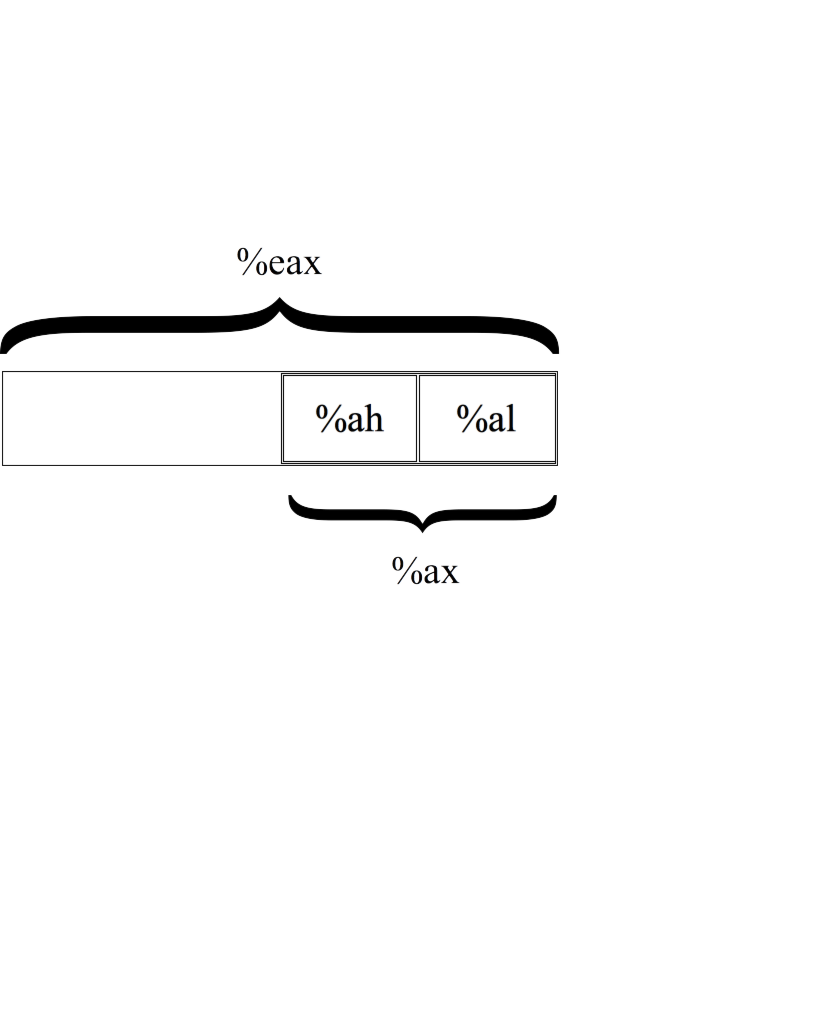
\includegraphics[width=\textwidth]{registerdescription.png}
\end{figure}

For a more comprehensive list of instructions, see \autoref{instructionsappendix}.

\section{Review}

\section{Know the Concepts}

\begin{itemize}\item What does it mean if a line in the program starts with the '\#' character? 
\item What is the difference between an assembly language file and an object code file? 
\item What does the linker do? 
\item How do you check the result status code of the last program you ran? 
\item What is the difference between \icode{movl \$1, {\eaxBare}} and \icode{movl 1, {\eaxBare}}? 
\item Which register holds the system call number? 
\item What are indexes used for? 
\item Why do indexes usually start at 0? 
\item If I issued the command \icode{movl data\_items(,{\ediBare},4), {\eaxBare}} and data\_items was address 3634 and {\ediReg} held the value 13, what address would you be using to move into {\eaxReg}? 
\item List the general-purpose registers. 
\item What is the difference between \icode{movl} and \icode{movb}? 
\item What is flow control? 
\item What does a conditional jump do? 
\item What things do you have to plan for when writing a program? 
\item Go through every instruction and list what addressing mode is being used for each operand. 
\end{itemize}

\section{Use the Concepts}

\begin{itemize}\item Modify the first program to return the value 3. 
\item Modify the \icode{maximum} program to find the minimum instead. 
\item Modify the \icode{maximum} program to use the number 255 to end the list rather than the number 0 
\item Modify the \icode{maximum} program to use an ending address rather than the number 0 to know when to stop. 
\item Modify the \icode{maximum} program to use a length count rather than the number 0 to know when to stop. 
\item What would the instruction \icode{movl \_start, {\eaxBare}} do?  Be specific, based on your knowledge of both addressing modes and the meaning of \icode{\_start}.  How would this differ from the instruction \icode{movl \$\_start, {\eaxBare}}? 
\end{itemize}

\section{Going Further}

\begin{itemize}\item Modify the first program to leave off the \icode{int} instruction line. Assemble, link, and execute the new program.  What error message do you get.  Why do you think this might be? 
\item So far, we have discussed three approaches to finding the end of the list - using a special number, using the ending address, and using the length count.  Which approach do you think is best?  Why?  Which approach would you use if you knew that the list was sorted?  Why? 
\end{itemize} 


\chapter{All About Functions}
\label{functionschapter}

% 
% 
% Copyright 2002 Jonathan Bartlett
% 
% Permission is granted to copy, distribute and/or modify this
% document under the terms of the GNU Free Documentation License,
% Version 1.1 or any later version published by the Free Software
% Foundation; with no Invariant Sections, with no Front-Cover Texts,
% and with no Back-Cover Texts.  A copy of the license is included in fdl.xml
% 

\section{Dealing with Complexity}

In \autoref{firstprogs}, the programs we wrote only consisted
of one section of code.  However, if we wrote real programs like that,
it would be impossible to maintain them.  It would be really difficult
to get multiple people working on the project, as any change in one part 
might adversely affect another part that another developer is working on.

To assist programmers in working together in groups, it is necessary
to break programs apart into separate pieces, which communicate with
each other through well-defined interfaces.  This way, each piece can
be developed and tested independently of the others, making it easier
for multiple programmers to work on the project.

Programmers use \emph{functions\index{functions}} to break their programs
into pieces which can be independently developed and tested.  Functions
are units of code that do a defined piece of work on specified types of 
data.  For example, in a word processor program, I may have a function called
\icode{handle\_typed\_character} which is activated whenever a
user types in a key.  The data the function uses would probably be the
keypress itself and the document the user currently has open.  The 
function would then modify the document according to the keypress it was 
told about.

The data items a function is given to process are called its 
\emph{parameters\index{parameters}}.  In the word processing example, the
key which was pressed and the document would be considered parameters 
to the \icode{handle\_typed\_characters} function.  The parameter
list and the processing expectations of a function (what it is expected to do
with the parameters) are called the function's interface.  Much care
goes into designing function interfaces, because if they
are called from many places within a project, it is difficult to change
them if necessary.

A typical program is composed of hundreds or thousands of functions, each with a 
small, well-defined task to perform.  However, ultimately there are things
that you cannot write functions for which must be provided by the system.
Those are called \emph{primitive functions\index{primitive functions}} (or just \emph{primitives\index{primitives}}) - they are the
basics which everything else is built off of.  For example, imagine a program
that draws a graphical user interface.  There has to be a function to create
the menus.  That function probably calls other functions to write text, to
write icons, to paint the background, calculate where the mouse pointer is,
etc.  However, ultimately, they will
reach a set of primitives provided by the operating system to do basic line
or point drawing.  Programming can either be viewed as breaking a large
program down into smaller pieces until you get to the primitive functions,
or incrementally building functions on top of primitives until you get the large picture
in focus.  In assembly language, the primitives are usually the same thing
as the system calls\index{system calls},
even though system calls aren't true functions as we will talk about in this chapter.

\section{How Functions Work}
\label{howfunctionswork}

Functions are composed of several different pieces:

\begin{description}
\item[function name] A function's name is a symbol\index{symbol}
that represents the address where the 
function's code starts.  In assembly language, the symbol is defined
by typing the function's name as a label
before the function's code.  This is just like labels\index{labels} you have used
for jumping.
\item[function parameters] A function's parameters\index{parameters}
are the data items that are explicitly
given to the function for processing.  For example, in mathematics,
there is a sine function.  If you were to ask a computer to find the sine
of 2, sine would be the function's name, and 2 would be the parameter.  Some
functions have many parameters, others have none.\footnote{Function parameters
can also be used to hold pointers to data that the function wants to send back to the
program.}
\item[local variables] Local variables\index{local variables} 
are data storage that a function uses
while processing that is thrown away when it returns.  It's kind of like
a scratch pad of paper.  Functions get a new piece of paper every time they
are activated, and they have to throw it away when they are
finished processing.  Local variables of a function are not accessible
to any other function within a program.
\item[static variables] Static variables\index{static variables} are data storage that a function
uses while processing that is not thrown away afterwards, but is
reused for every time the function's code is activated.  This data
is not accessible to any other part of the program.  Static
variables are generally  not used unless absolutely necessary, as they
can cause problems later on.
\item[global variables] Global variables
are data storage that a function uses for processing
which are managed outside the function.  For example, a simple text editor
may put the entire contents of the file it is working on in a global
variable so it doesn't have to be passed to every function that operates
on it.\footnote{This is generally considered bad practice.  Imagine
if a program is written this way, and in the next version they decided
to allow a single instance of the program edit multiple files.  Each function
would then have to be modified so that the file that was being manipulated
would be passed as a parameter.  If you had simply passed it as a parameter
to begin with, most of your functions could have survived your upgrade
unchanged.}  Configuration values are also often stored in
global variables.
\item[return address] The return address\index{return address} 
is an "invisible" parameter in that it isn't directly used during the function.
The return address is a parameter which tells the function where to resume
executing after the function is completed.   This is needed because 
functions can be
called to do processing from many different parts of your program, and
the function needs to be able to get back to wherever it was called
from.  In most programming languages, this parameter
is passed automatically when the function is called.  In assembly language,
the \icode{call\index{call}} instruction handles passing
the return address for you, and \icode{ret\index{ret}} handles
using that address to return back to where you called the function from.
\item[return value] The return value\index{return value} is the 
main method of transferring data back to the
main program.  Most programming languages only allow a single return value 
for a function.
\end{description}

\index{global variables} 
These pieces are present in most programming languages.  How you specify
each piece is different in each one, however.

The way that the variables are stored and the parameters and return values
are transferred by the computer varies from language to language as well.  
This variance is  known as
a language's \emph{calling convention}\index{calling
conventions}, because it describes how functions expect
to get and receive data when they are called.\footnote{A 
\emph{convention} is a way of doing things that is standardized,
but not forcibly so.  For example, it is a convention for people to shake
hands when they meet.  If I refuse to shake hands with you, you may think
I don't like you.  Following conventions is important because it makes it
easier for others to understand what you are doing, and makes it easier
for programs written by multiple independent authors to work together.
}

Assembly language can use any calling convention it wants to.  
You can even make one up yourself.  However, if
you want to interoperate with functions written in other 
languages, you have to obey their calling conventions.  We 
will use the calling convention of the C programming language\index{C programming language} 
for our examples because it is the most widely used, and because it is the standard for Linux platforms.

\section{Assembly-Language Functions using the C Calling Convention}
\label{callingwritingassemblyfunctions}

You cannot write assembly-language functions without understanding
how the computer's \emph{stack\index{stack}} works.  Each computer
program that runs uses a region of memory called the stack to enable
functions to work properly.  Think of a stack as a pile of papers
on your desk which can be added to indefinitely.  You generally keep
the things that you are working on toward the top, and you take things
off as you are finished working with them.

Your computer has a stack, too.  The computer's stack\index{stack} lives at the very 
top addresses of memory.  You can push values onto the 
top of the stack through an instruction called
\icode{pushl\index{pushl}}, which pushes either a register or
memory value onto the top of the stack.  Well, we say it's the top, but the
"top" of the stack is actually the bottom of the stack's memory.  
Although this is confusing, the reason for it is that when we think
of a stack of anything - dishes, papers, etc. - we think of adding and 
removing to the top of it.  However,
in memory the stack starts at the top of memory and grows downward due
to architectural considerations.  Therefore, when we refer to the
"top of the stack" remember it's at the bottom of the stack's memory\index{stack memory}.  
You can also pop values off the top using an instruction called
\icode{popl\index{popl}}.
This removes the top value from the stack and places it into a register or memory location of your choosing..

When we push a value onto the stack, the top of the stack moves 
to accomodate the additional value.  We can actually continually 
push values onto the stack and it will keep growing further and
further down in memory until we hit our code or data.
So how do we know where the current "top" of the stack is?  The
stack register\index{stack register}, {\espRegIdx}, always contains a pointer\index{pointer} to the current top of the stack, wherever it is.

Every time we push something onto the stack with \icode{pushl}, 
{\espReg} gets subtracted by 4 so that it points to the new top of the stack 
(remember, each word is four bytes long, and the stack grows downward).  
If we want to remove something from the stack, we simply use the 
\icode{popl} instruction, which adds 4 to {\espReg} and puts the 
previous top value in whatever register you specified.  
\icode{pushl} and \icode{popl} each
take one operand - the register to push onto the stack for 
\icode{pushl}, or receive the data that is popped off the stack
for \icode{popl}.

If we simply want to access the value on the top of the stack without removing it,
we can simply use the {\espRegIdx} register in indirect addressing mode\index{indirect addressing mode}.  For example, the 
following code moves whatever is at the top of the stack into
{\eaxReg}:

\begin{simpletyping}
\begin{lstlisting}
movl ({\espBare}), {\eaxBare}
\end{lstlisting}
\end{simpletyping}

If we were to just do this:

\begin{simpletyping}
\begin{lstlisting}
movl {\espBare}, {\eaxBare}
\end{lstlisting}
\end{simpletyping}

then {\eaxReg} would just hold the pointer to the top of the stack rather than
the value at the top.  Putting {\espReg} in parenthesis causes the computer to
go to indirect addressing mode\index{indirect addressing mode},
and therefore we get the value pointed to by {\espRegIdx}.  If we want to 
access the value right below the top of the stack, we can simply issue this instruction:

\begin{simpletyping}
\begin{lstlisting}
movl 4({\espBare}), {\eaxBare}
\end{lstlisting}
\end{simpletyping}

This instruction uses the base pointer addressing mode\index{base pointer addressing mode}
(see \autoref{dataaccessingmethods})
which simply adds 4 to {\espRegIdx} before looking up the value being pointed to.  

In the C language calling convention\index{C language calling convention}, the stack is the key 
element for implementing a function's local variables, 
parameters, and return address. 

Before executing a function\index{functions},
a program pushes all of the parameters\index{parameters} for the function onto
the stack in the reverse order that they are documented.  Then
the program issues a \icode{call\index{call}} instruction
indicating which function it wishes to start.  The 
\icode{call} instruction does two things.  First
it pushes the address of the next instruction, which is the
return address\index{return address}, onto the stack\index{stack}.  Then it modifies the 
instruction pointer\index{instruction pointer} ({\eipRegIdx})
to point to the start of the function.  So, at the time the
function starts, the stack looks like this (the "top" of the stack is
at the bottom on this example):

%  FIXME - Dominique says "This part can be confusing until one gets to the sample illustration code and then it makes sense." 

\begin{simpletyping}
\begin{lstlisting}
Parameter \#N
...
Parameter 2
Parameter 1
Return Address <--- ({\espBare})
\end{lstlisting}
\end{simpletyping}

Each of the parameters of the function have been pushed onto the stack,
and finally the return address is there.
Now the function itself has some work to do.  

The first thing
it does is save the current base pointer register\index{base pointer register},
 {\ebpRegIdx}, by doing
\icode{pushl {\ebpBare}}.  The base pointer is a special register\index{special register} used for accessing function parameters\index{function parameters} and local variables\index{local variables}.
Next, it copies the stack pointer\index{stack pointer}
to {\ebpRegIdx} by doing \icode{movl {\espBare}, {\ebpBare}}.  This 
allows you to be able to access the function parameters
as fixed indexes from the base pointer.  You may think that you can
use the stack pointer for this.  However, during your
program you may do other things with the stack such as pushing
arguments to other functions.

Copying the stack pointer into
the base pointer at the beginning of a function allows you to always 
know where your parameters are (and as we will see, local variables too),
even while you may be pushing things on and off the stack.  {\ebpRegIdx}
will always be where the stack pointer was at the beginning of the function,
so it is more or less a constant reference to the \emph{stack frame\index{stack frame}} (the stack frame
consists of all of the stack variables used within a function, including 
parameters\index{parameters}, local variables\index{local variables}, and the return address\index{return address}).

At this point, the stack looks like this:

\begin{simpletyping}
\begin{lstlisting}
Parameter \#N   <--- N*4+4({\ebpBare})
...
Parameter 2    <--- 12({\ebpBare})
Parameter 1    <--- 8({\ebpBare})
Return Address <--- 4({\ebpBare})
Old {\ebpBare}       <--- ({\espBare}) and ({\ebpBare})
\end{lstlisting}
\end{simpletyping}

As you can see, each parameter can be accessed using base pointer addressing mode\index{base pointer addressing mode} using the {\ebpRegIdx} register.

Next, the function reserves space on the stack for any local
variables\index{local variables} it needs.
This is done by simply moving the stack pointer\index{stack pointer} out of the way.
Let's say that we are going to need two words of memory
to run a function.  We can simply move the stack pointer down two
words to reserve the space.  This is done like this:

\begin{simpletyping}
\begin{lstlisting}
subl \$8, {\espBare}
\end{lstlisting}
\end{simpletyping}

This subtracts 8 from {\espReg} (remember, a word is four bytes 
long).\footnote{Just a reminder - the dollar sign in
front of the eight indicates immediate mode addressing\index{immediate mode addressing}, meaning
that we subtract the number 8 itself from {\espReg} rather than the value at
address 8.}  This way, we can use the stack for
variable storage without worring about clobbering them with pushes
that we may make for function calls.  Also, since it is allocated on 
the stack frame for this function call, the variable will only be 
alive during this function.  When we return, the stack frame will go
away, and so will these variables.  That's why they are called local -
they only exist while this function is being called.

Now we have two words for local storage.  Our stack now looks like this:

\begin{simpletyping}
\begin{lstlisting}
Parameter \#N     <--- N*4+4({\ebpBare})
...
Parameter 2      <--- 12({\ebpBare})
Parameter 1      <--- 8({\ebpBare})
Return Address   <--- 4({\ebpBare})
Old {\ebpBare}         <--- ({\ebpBare})
Local Variable 1 <--- -4({\ebpBare})
Local Variable 2 <--- -8({\ebpBare}) and ({\espBare})
\end{lstlisting}
\end{simpletyping}

So we can now access all of the data we need for this function
by using base pointer addressing\index{base pointer addressing mode} using different offsets from {\ebpRegIdx}.
{\ebpRegIdx} was made specifically for this purpose, 
which is why it is called the base pointer\index{base pointer register}.  You can use other
registers in base pointer addressing mode, but the x86 architecture
makes using the {\ebpRegIdx} register a lot faster.

\index{static variables}
\index{global variables} 
Global variables and static variables are accessed just like the memory
we have been accessing memory in previous chapters.  The only difference
between the global and static variables is that static variables are 
only used by one function, while global variables are used by 
many functions. Assembly language treats them exactly the same, 
although most other languages distinguish them.

When a function is done executing, it does three things:

\begin{enumerate}\item It stores its return value in {\eaxRegIdx}. 
\item It resets the stack to what it was when it was called (it gets rid of the current stack frame\index{stack frame} and puts the stack frame of the calling code back into effect). 
\item It returns control back to wherever it was called from.  This is done using the 
\icode{ret\index{ret}} instruction, which pops whatever
value is at the top of the stack, and sets the instruction pointer\index{instruction pointer}, 
{\eipRegIdx}, to that value. 
\end{enumerate}

So, before a function returns control to the code that called it, it
must restore the previous stack frame.  Note also that without doing this,
\icode{ret} wouldn't work, because in our current stack
frame, the return address is not at the top of the stack.  Therefore, before
we return, we have to reset the stack pointer\index{stack pointer} {\espRegIdx} and base pointer\index{base pointer} {\ebpRegIdx} to what they
were when the function began.

Therefore to return from the function you have to do the following:

\begin{simpletyping}
\begin{lstlisting}
movl {\ebpBare}, {\espBare}
popl {\ebpBare}
ret
\end{lstlisting}
\end{simpletyping}

\emph{At this point, you should consider all local variables to be 
disposed of.}  The reason is that after you move the stack
pointer back, future stack pushes will likely overwrite everything
you put there.  Therefore, you should never save the address
of a local variable\index{local variables} past the life of the function it was 
created in, or else it will be overwritten after the life of its stack 
frame ends.  

Control has now been handed back to the calling code,
which can now examine {\eaxRegIdx} for the return value\index{return value}.  The calling
code also needs to pop off all of the parameters it 
pushed onto the stack in order to get the stack pointer\index{stack pointer}
back where it was (you can also simply add 4 * number of parameters
to {\espRegIdx} using the \icode{addl} instruction, if 
you don't need the values of the parameters anymore).\footnote{This is not always strictly needed unless you are saving registers on the stack before a function call.  The base pointer keeps the stack frame in a reasonably consistent state.  However, it is still a good idea, and is absolutely necessary if you are temporarily saving registers on the stack..}

\begin{sidebar}[Destruction of Registers]
When you call a function\index{functions}, you should assume that everything
currently in your registers\index{registers} will be wiped out.  The only
register that is guaranteed to be left with the value it
started with are {\ebpRegIdx} and a few others (the Linux C calling 
convention requires functions to preserve the values of {\ebxRegIdx}, 
{\ediRegIdx}, and {\esiRegIdx} if they are altered - this is not
strictly held during this book because these programs are self-contained
and not called by outside functions).  {\ebxReg} also has some other uses
in position-independent code, which is not covered in this book.
{\eaxRegIdx} is guaranteed to be overwritten with the return value,
and the others likely are.  If there are registers you want
to save before calling a function, you need to save them by
pushing them on the stack\index{stack} before pushing the function's 
parameters.  You can then pop them back off in reverse order
after popping off the parameters.  Even if you know a function
does not overwrite a register you should save it, because
future versions of that function may.

Note that in Linux assembly language,
functions are 

Other languages' calling 
conventions\index{calling conventions}
may be different.  For example, other calling conventions may
place the burden on the function to save any registers it uses.  Be sure
to check to make sure the calling conventions of your languages 
are compatible before trying to mix languages.  Or in the case of assembly
language, be sure you know how to call the other language's functions.
\end{sidebar}

\begin{sidebar}[Extended Specification]
Details of the C language calling convention\index{calling convention} 
(also known as the ABI\index{ABI}, or 
Application Binary Interface\index{Application Binary Interface}) is available online.  We have oversimplified and left
out several important pieces to make this simpler for new programmers.
For full details, you should check out the documents available at
http://www.linuxbase.org/spec/refspecs/  Specifically, you should look
for the \documentname{System V Application Binary Interface - Intel386
Architecture Processor Supplement}.
\end{sidebar}

\section{A Function Example}

Let's take a look at how a function call\index{function call} works in a real program.  The
function we are going to write is the \icode{power}
function.  We will give the power function two parameters -
the number and the power we want to raise it to.  For example,
if we gave it the parameters 2 and 3, it would raise 2 to the
power of 3, or 2*2*2, giving 8.  In order to make this
program simple, we will only allow numbers 1 and greater.

The following is the code for the complete program.  As usual,
an explanation follows.  Name the file \icode{power.s}.

\begin{simpletyping}
\lstinputlisting{power.s}
\end{simpletyping}

Type in the program, assemble it, and run it.  Try calling
power for different values, but remember that the result
has to be less than 256 when it is passed back to the operating
system.  Also try subtracting the results of the two 
computations.  Try adding a third call to the 
\icode{power} function, and add its result
back in.  

The main program code is pretty simple.  You push the 
arguments onto the stack, call the function, and then move
the stack pointer back.  The result is stored in {\eaxReg}.
Note that between the two calls to \icode{power},
we save the first value onto the stack.  This is because the
only register that is guaranteed to be saved is {\ebpRegIdx}.
Therefore we push the value onto the stack, and pop the value 
back off after the second function call is complete.

Let's look at how the function itself is written.  Notice
that before the function, there is documentation as to
what the function does, what its arguments are, and
what it gives as a return value.  This is useful for 
programmers who use this function.  This is the function's
interface.  This lets the programmer know what values are
needed on the stack, and what will be in {\eaxReg} at the end.

We then have the following line:

\begin{simpletyping}
\begin{lstlisting}
	.type power,@function
\end{lstlisting}
\end{simpletyping}

\index{.type}
\index{@functions}
This tells the linker that the symbol \icode{power}
should be treated as a function.  Since this program
is only in one file, it would work just the same with this
left out.  However, it is good practice.

After that, we define the value of the \icode{power} label:

\begin{simpletyping}
\begin{lstlisting}
power:
\end{lstlisting}
\end{simpletyping}

As mentioned previously, this defines the symbol 
\icode{power} to be the address where the instructions
following the label begin.  This is how 
\icode{call power} works.  It transfers control to
this spot of the program.  The difference between 
\icode{call\index{call}} and \icode{jmp\index{jmp}} is that 
\icode{call} also pushes the return address onto
the stack so that the function can return, while the 
\icode{jmp} does not.

Next, we have our instructions to set up our function:

\begin{simpletyping}
\begin{lstlisting}
	pushl {\ebpBare}
	movl  {\espBare}, {\ebpBare}
	subl  \$4, {\espBare}
\end{lstlisting}
\end{simpletyping}

At this point, our stack looks like this:

\begin{simpletyping}
\begin{lstlisting}
Base Number    <--- 12({\ebpBare})
Power          <--- 8({\ebpBare})
Return Address <--- 4({\ebpBare})
Old {\ebpBare}       <--- ({\ebpBare})
Current result <--- -4({\ebpBare}) and ({\espBare})
\end{lstlisting}
\end{simpletyping}

Although we could use a register for temporary storage, this
program uses a 
local variable\index{local variables}
in order to show how to set it
up.  Often times there just aren't enough registers to store
everything, so you have to offload them into local variables.
Other times, your function will need to call another function
and send it a pointer to some of your data.  You can't have
a pointer\index{pointer} 
to a register\index{register}, 
so you have to store it in a 
local variable in order to send a pointer to it.

Basically, what the program does is start with the base number,
and store it both as the multiplier (stored in {\ebxReg}) and the 
current value (stored in -4({\ebpBare})).  It also has the power
stored in {\ecxReg}  It then continually 
multiplies the current value by the multiplier, decreases 
the power, and leaves the loop if the power (in {\ecxReg}) gets down to 1.

By now, you should be able to go through the program without
help.  The only things you should need to know is that
\icode{imull\index{imull}} does integer multiplication and stores
the result in the second operand, and \icode{decl\index{decl}}
decreases the given register by 1.  For more information on these
and other instructions, see \autoref{instructionsappendix}

A good project to try now is to extend the program so it
will return the value of a number if the power is 0 (hint,
anything raised to the zero power is 1).  Keep trying.
If it doesn't work at first, try going through your program
by hand with a scrap of paper, keeping track of where
{\ebpReg} and {\espReg} are pointing, what is on the stack, and what the
values are in each register.

\section{Recursive Functions}
\label{recursivefunctions}

The next program will stretch your brains even
more.  The program will compute the 
\emph{factorial} of a number.  A
factorial is the product of a number and all the numbers between it
and one.  For example, the factorial of 7 is 7*6*5*4*3*2*1, and the
factorial of 4 is 4*3*2*1.  Now, one thing you might notice is that
the factorial of a number is the same as the product of a number and
the factorial just below it.  For example, the factorial of 4 is
4 times the factorial of 3.  The factorial of 3 is 3 times the factorial
of 2.  2 is 2 times the factorial of 1.  The factorial of 1 is 1.  
This type of definition is called a recursive\index{recursive} definition.  That means,
the definition of the factorial function\index{functions} includes the factorial function itself. 
However, since all functions need to end, a recursive definition must
include a \emph{base case\index{base case}}.  The base case is the
point where recursion will stop.  Without a base case, the function would
go on forever calling itself until it eventually ran out of stack space.  
In the case of the factorial, the base case
is the number 1.  When we hit the number 1, we don't run the factorial
again, we just say that the factorial of 1 is 1.  So, let's run through
what we want the code to look like for our factorial 
function:

\begin{enumerate}\item Examine the number 
\item Is the number 1? 
\item If so, the answer is one 
\item Otherwise, the answer is the number times the factorial of the number minus one 
\end{enumerate}

This would be problematic if we didn't have local variables\index{local variables}.
In other programs, storing values in global variables worked fine.  However,
global variables only provide one copy of each variable.  In this program,
we will have multiple copies of the function running at the same time, all
of them needing their own copies of the data!\footnote{By "running
at the same time" I am talking about the fact that one will not have
finished before a new one is activated.  I am not implying that their
instructions are running at the same time.}
Since local variables exist on the stack frame, and each function call
gets its own stack frame\index{stack frame}, we are okay.

Let's look at the code to see how this works:

\begin{simpletyping}
\lstinputlisting{factorial.s}
\end{simpletyping}

Assemble, link, and run it with these commands:

\begin{simpletyping}
\begin{lstlisting}
as factorial.s -o factorial.o
ld factorial.o -o factorial
./factorial
echo \$?
\end{lstlisting}
\end{simpletyping}

This should give you the value 24.  24 is the factorial of 4, you can
test it out yourself with a calculator: 4 * 3 * 2 * 1 = 24.

I'm guessing you didn't understand the whole code listing.  Let's go
through it a line at a time to see what is happening. 

\begin{simpletyping}
\begin{lstlisting}
\_start:
	pushl \$4
	call factorial
\end{lstlisting}
\end{simpletyping}

Okay, this program is intended to compute the factorial of the number 
4.  When programming functions, you are supposed to put the
parameters\index{parameters} of the function on the top of the stack right before
you call it.  Remember, a function's \emph{parameters\index{parameters}}
are the data that you want the function to work with.  In this case,
the factorial function takes 1 parameter - the number you want the
factorial of.  

The \icode{pushl\index{pushl}}
instruction puts the given value at the top of the stack.  
The \icode{call\index{call}} instruction then makes the function call.

Next we have these lines:

\begin{simpletyping}
\begin{lstlisting}
        addl  \$4, {\espBare}
        movl  {\eaxBare}, {\ebxBare}
        movl  \$1, {\eaxBare}
        int   \$0x80
\end{lstlisting}
\end{simpletyping}

This takes place after \icode{factorial} has finished and computed
the factorial of 4 for us.  Now we have to clean up the stack.
The \icode{addl} instruction moves the stack pointer back
to where it was before we pushed the \icode{\$4} onto the stack.
You should always clean up your stack parameters after a function call returns.

The next instruction moves {\eaxReg} to
{\ebxReg}.  What's in {\eaxRegIdx}?  It is
\icode{factorial}'s return value\index{return value}.  
In our case, it is the value of the factorial function.  With 4 as our
parameter, 24 should be our return value.  Remember, return values are
always stored in {\eaxRegIdx}.  We want to return this value as the
status code to the operating system.  However,
Linux requires that the program's exit status be stored in
{\ebxRegIdx}, not {\eaxReg}, so we have to
move it.  Then we do the standard exit system call.

The nice thing about function calls is that:

\begin{itemize}
\item Other programmers don't have to know anything about them except its arguments to use them. 
\item They provide standardized building blocks from which you can form a program. 
\item They can be called multiple times and from multiple locations and they always know how to get back to where they were since \icode{call\index{call}} pushes the return address onto the stack. 
\end{itemize}

These are the main advantages of functions.  
Larger programs also use functions to break 
down complex pieces of code into smaller, simpler ones.  In fact, almost
all of programming is writing and calling functions. 

Let's now take a look at how the \icode{factorial} 
function itself is implemented.

Before the function starts, we have this directive:

\begin{simpletyping}
\begin{lstlisting}
	.type factorial,@function
factorial:
\end{lstlisting}
\end{simpletyping}

The \icode{.type\index{.type}} directive tells the linker that 
\icode{factorial} is a function.  This isn't really needed
unless we were using \icode{factorial} in other programs.
We have included it for completeness.  The line that says 
\icode{factorial:} gives the symbol \icode{factorial}
the storage location of the next instruction.  That's how 
\icode{call} knew where to go when we said 
\icode{call factorial}.  

The first real instructions of the function are:

\begin{simpletyping}
\begin{lstlisting}
	pushl {\ebpBare}
	movl  {\espBare}, {\ebpBare}
\end{lstlisting}
\end{simpletyping}

As shown in the previous program, this creates the stack frame\index{stack frame}
for this function.  These two lines will be the way you should
start every function.

The next instruction is this:

\begin{simpletyping}
\begin{lstlisting}
	movl  8({\ebpBare}), {\eaxBare}
\end{lstlisting}
\end{simpletyping}

This uses base pointer addressing\index{base pointer addressing mode} to move the first parameter\index{parameter}
of the function into {\eaxReg}.  Remember, \icode{({\ebpBare})}
has the old {\ebpReg}, \icode{4({\ebpBare})} has the return address,
and \icode{8({\ebpBare})} is the location of the first parameter 
to the function.  If you think back, this will be the value 4
on the first call, since
that was what we pushed on the stack before calling the function the
first time (with \icode{pushl \$4}).  As this function calls itself,
it will have other values, too.

Next, we check to see if we've hit our base case (a parameter of 1).  If
so, we jump to the instruction at the label \icode{end\_factorial},
where it will be returned.  It's already in {\eaxReg} which
we mentioned earlier is where you put return values\index{return values}.  That is accomplished
by these lines:

\begin{simpletyping}
\begin{lstlisting}
	cmpl \$1, {\eaxBare}
	je end\_factorial
\end{lstlisting}
\end{simpletyping}

If it's not our base case, what did we say we would do?  We would call
the \icode{factorial} function again with our parameter minus
one.  So, first we decrease {\eaxReg} by one:

\begin{simpletyping}
\begin{lstlisting}
	decl {\eaxBare}
\end{lstlisting}
\end{simpletyping}

\icode{decl\index{decl}} stands for decrement.  It subtracts 1 from
the given register or memory location ({\eaxReg} in our case).  
\icode{incl\index{incl}} is the
inverse - it adds 1.  After decrementing {\eaxReg}
we push it onto the stack since it's going to be the parameter of
the next function call.  And then we call \icode{factorial} again!

\begin{simpletyping}
\begin{lstlisting}
	pushl {\eaxBare}
	call factorial
\end{lstlisting}
\end{simpletyping}

Okay, now we've called \icode{factorial}.  One thing to remember 
is that after a function call, we can never know what the registers are
(except \icode{{\espBare}} and \icode{{\ebpBare}}).  So
even though we had the value we were called with in \icode{{\eaxBare}},
it's not there any more.  Therefore, we need pull it off the stack
from the same place we got it the first time (at 
\icode{8({\ebpBare})}).
So, we do this:

\begin{simpletyping}
\begin{lstlisting}
	movl 8({\ebpBare}), {\ebxBare}
\end{lstlisting}
\end{simpletyping}

Now, we want to multiply that number with the result of the
factorial function.  If you remember our previous discussion,
the result of functions are left in {\eaxReg}.
So, we need to multiply {\ebxReg} with {\eaxReg}.
This is done with this instruction:

\begin{simpletyping}
\begin{lstlisting}
	imull {\ebxBare}, {\eaxBare}
\end{lstlisting}
\end{simpletyping}

This also stores the result in {\eaxReg}, which is
exactly where we want the return value for the function to be!  Since
the return value\index{return value} is in place
we just need to leave the function.  If you remember, at the
start of the function we pushed {\ebpReg}, and
moved {\espReg} into {\ebpReg} to create the current stack frame.  Now
we reverse the operation to destroy the current stack frame and 
reactivate the last one:

\begin{simpletyping}
\begin{lstlisting}
end\_factorial:
	movl {\ebpBare}, {\espBare}
	popl {\ebpBare}
\end{lstlisting}
\end{simpletyping}

Now we're already to return, so we issue the following command

\begin{simpletyping}
\begin{lstlisting}
	ret
\end{lstlisting}
\end{simpletyping}

This pops the top value off of the stack, and then jumps to it.  If
you remember our discussion about \icode{call}, we said
that \icode{call\index{call}} first pushed the address of the
next instruction onto the stack before it jumped to the beginning
of the function.  So, here we pop it back off so we can return there.
The function is done, and we have our answer!  

Like our previous program, you should look over the
program again, and make sure you know what everything does.
Look back through this section and the previous sections for the 
explanation of anything you don't understand.  Then, take a 
piece of paper, and go through the program
step-by-step, keeping track of what the values of the registers
are at each step, and what values are on the stack.  Doing this
should deepen your understanding of what is going on.

\section{Review}

\section{Know the Concepts}

\begin{itemize}\item What are primitives? 
\item What are calling conventions? 
\item What is the stack? 
\item How do \icode{pushl} and \icode{popl} affect the stack?  What special-purpose register do they affect? 
\item What are local variables and what are they used for? 
\item Why are local variables so necessary in recursive functions? 
\item What are {\ebpReg} and {\espReg} used for? 
\item What is a stack frame? 
\end{itemize}

\section{Use the Concepts}
\label{functionsreviewuseconcepts}

\begin{itemize}\item Write a function called \icode{square} which receives one argument and returns the square of that argument. 
\item Write a program to test your \icode{square} function. 
\item Convert the maximum program given in \autoref{maximum} so that it is a function which takes a pointer to several values and returns their maximum.  Write a program that calls maximum with 3 different lists, and returns the result of the last one as the program's exit status code. 
\item Explain the problems that would arise without a standard calling convention. 
\end{itemize}

\section{Going Further}

\begin{itemize}\item Do you think it's better for a system to have a large set of primitives or a small one, assuming that the larger set can be written in terms of the smaller one? 
\item The factorial function can be written non-recursively.  Do so. 
\item Find an application on the computer you use regularly.  Try to locate a specific feature, and practice breaking that feature out into functions.  Define the function interfaces between that feature and the rest of the program. 
\item Come up with your own calling convention.  Rewrite the programs in this chapter using it.  An example of a different calling convention would be to pass parameters in registers rather than the stack, to pass them in a different order, to return values in other registers or memory locations.  Whatever you pick, be consistent and apply it throughout the whole program. 
\item Can you build a calling convention without using the stack?  What limitations might it have? 
\item What test cases should we use in our example program to check to see if it is working properly? 
\end{itemize}


\chapter{Dealing with Files}
\label{filesch}

% 
% 
% Copyright 2002 Jonathan Bartlett
% 
% Permission is granted to copy, distribute and/or modify this
% document under the terms of the GNU Free Documentation License,
% Version 1.1 or any later version published by the Free Software
% Foundation; with no Invariant Sections, with no Front-Cover Texts,
% and with no Back-Cover Texts.  A copy of the license is included in fdl.xml
% 

A lot of computer programming deals with files\index{files}.  After all, when we reboot our
computers, the only thing that remains from previous sessions are 
the things that have been put on disk.  Data which is stored in 
files is called \emph{persistent\index{persistance}} data, 
because it persists in files that remain on the disk even when the program isn't running..

\section{The UNIX File Concept}

Each operating system has its own way of dealing with files.  However, the
UNIX method, which is used on Linux, is the simplest and most universal.
UNIX files, no matter what program created them, can all be accessed as a 
sequential stream of bytes.  When you access a file, you start by opening it by name.
The operating system then gives you a number, called a 
\emph{file descriptor\index{file descriptors}}, 
which you use to refer to the file until you are
through with it.  You can then read and write to the file using its
file descriptor.  When you are done reading and writing, you then close 
the file, which then makes the file descriptor useless.

In our programs we will deal with files in the following ways:

\begin{enumerate}
\item Tell Linux the name of the file to open, and in what mode you want it 
opened (read, write, both read and write, create it if it doesn't exist, 
etc.).  This is handled with the 
\icode{open\index{open}} 
system call, which takes a filename, a number representing the mode, 
and a permission\index{permissions} set as its parameters.  {\eaxRegIdx} will hold the system call number, which is 5.
The address of the first character of the filename should be stored
in {\ebxRegIdx}.  The read/write intentions, represented as 
a number, should be stored in {\ecxRegIdx}.  For now, use 0 for files you want to read
from, and 03101 for files you want to write to 
(you must include the leading zero).\footnote{This will be explained 
in more detail in \autoref{truthbinarynumbers}.}  
Finally, the permission set should be stored as a number in {\edxRegIdx}.  
If you are unfamiliar with UNIX permissions, just use 0666 for the 
permissions (again, you must include the leading zero). 
\item Linux will then return to you a file descriptor\index{file descriptors} in 
{\eaxRegIdx}.  Remember, this is a number that you use to refer to this file 
throughout your program. 
\item Next you will operate on the file doing reads and/or writes, each time 
giving Linux the file descriptor you want to use.  \icode{read\index{read}}
is system call 3, and to call it you need to have the file descriptor
in {\ebxReg}, the address of a buffer for storing the 
data that is read in {\ecxReg}, and the size of the buffer in {\edxReg}.  
Buffers will be explained in \autoref{buffersbss}.
\icode{read} will return with either the number of 
characters read from the file, or an error code.  Error codes can be
distinguished because they are always negative numbers (more information
on negative numbers can be found in \autoref{countingchapter}).  
\icode{write\index{write}} 
is system call 4, and it requires the same 
parameters as the \icode{read} system call, except that the
buffer should already be filled with the data to write out.  The 
\icode{write} system call will give back the number
of bytes written in {\eaxReg} or an error code. 
\item When you are through with your files, you can then tell Linux to close them.  
Afterwards, your file descriptor\index{file descriptors} is no longer valid.
This is done using \icode{close\index{close}}, system call 6.  The only
parameter to \icode{close} is the file descriptor, which is
placed in {\ebxReg} 
\end{enumerate}

\section{Buffers and \icode{.bss}}
\label{buffersbss}

In the previous section we mentioned buffers\index{buffers} without explaining what they
were.  A buffer is a continuous block of bytes used for bulk data transfer.
When you request to read a file, the operating system needs to have a place
to store the data it reads.  That place is called a buffer.   Usually buffers
are only used to store data temporarily, and it is then read from the buffers
and converted to a form that is easier for the programs to handle.  Our
programs won't be complicated enough to need that done.
For an example, let's say that you want to read in a single line of text from
a file but you do not know how long that line is.  You would then
simply read a large number of bytes/characters from the file into a buffer, 
look for the end-of-line character, and copy all of the characters to that
end-of-line character to another location.  If you didn't find an end-of-line
character, you would allocate another buffer and continue reading.
You would probably wind up with some characters left over in your buffer
in this case, which you would use as the starting point when you next need
data from the file.\footnote{While this sounds complicated, most of 
the time in programming you will not need to deal directly with buffers
and file descriptors.  In \autoref{linking} you will learn how
to use existing code present in Linux to handle most of the complications
of file input/output for you.}

Another thing to note is that buffers\index{buffers} are a fixed size, set by the programmer.
So, if you want to read in data 500 bytes at a time, you send the 
\icode{read} system call the address of a 500-byte unused location,
and send it the number 500 so it knows how big it is.  You can make it smaller
or bigger, depending on your application's needs.  

To create a buffer, you need to either reserve static or dynamic storage.
Static storage is what we have talked about so far, storage locations
declared using \icode{.long} or \icode{.byte} directives.
Dynamic storage will be discussed in \autoref{dynamicmemory}.  
There are problems, though, with declaring buffers using \icode{.byte\index{.byte}}.
First, it is tedious to type.  You would have to type 500 numbers after
the \icode{.byte} declaration, and they wouldn't be used
for anything but to take up space.
Second, it uses up space in the executable.  In the examples we've
used so far, it doesn't use up too much, but that can change in larger 
programs.  If you want 500 bytes you have to type in 500 numbers and it 
wastes 500
bytes in the executable.  There is a solution to both of these.  So far,
we have discussed two program sections, the \icode{.text\index{.text}} and
the \icode{.data\index{.data}} sections.  There is another section called
the \icode{.bss\index{.bss}}.  This section is like the data section, except
that it doesn't take up space in the executable.  This section can
reserve storage, but it can't initialize it.  In the \icode{.data}
section, you could reserve storage and set it to an initial value.  In the
\icode{.bss} section, you can't set an initial value.  This is
useful for buffers because we don't need to initialize them anyway, we
just need to reserve storage.  In order to do this, we do the following
commands:

\begin{simpletyping}
\begin{lstlisting}
.section .bss
	.lcomm my\_buffer, 500
\end{lstlisting}
\end{simpletyping}

This directive, \icode{.lcomm\index{.lcomm}}, will create a symbol, \icode{my\_buffer}, that refers to 
a 500-byte storage location that we can use as a buffer.  We can then do
the following, assuming we have opened a file for reading and have placed
the file descriptor in {\ebxReg}:

\begin{simpletyping}
\begin{lstlisting}
	movl \$my\_buffer, {\ecxBare}
	movl 500, {\edxBare}
	movl 3, {\eaxBare}
	int  \$0x80
\end{lstlisting}
\end{simpletyping}

This will read up to 500 bytes into our buffer.  In this example, I placed
a dollar sign in front of \icode{my\_buffer}.  Remember that the 
reason for this is that without the dollar sign, 
\icode{my\_buffer} is treated as a memory location, and is
accessed in direct addressing mode\index{direct addressing mode}.  The dollar sign switches it to immediate mode addressing,
which actually loads the number represented by \icode{my\_buffer} 
itself (i.e. - the address of the start of our buffer, which is the address 
of \icode{my\_buffer}) into {\ecxReg}.

\section{Standard and Special Files}

You might think that programs start without any files open by default.  This
is not true.  Linux programs usually have at least three open file descriptors\index{file descriptors} 
when they begin.  They are:

\begin{description}
\item[STDIN\index{STDIN}] This is the \emph{standard input\index{standard input}}.  It is a read-only file, and 
usually represents your keyboard.\footnote{As we mentioned earlier, in Linux, almost everything is a "file".  Your keyboard input is considered a file, and so is your screen display.
}
This is always file descriptor 0.
\item[STDOUT\index{STDOUT}] This is the \emph{standard output\index{standard output}}.  It is a write-only file, 
and usually represents your screen display.  This is always file descriptor 1.
\item[STDERR\index{STDERR}] This is your \emph{standard error\index{standard error}}.  It is a write-only file, 
and usually represents your screen display.  Most regular processing 
output goes to \icode{STDOUT}, but any error messages that come 
up in the process go to \icode{STDERR}.  This way, if you want to, 
you can split them up into separate places.  This is always file
descriptor 2.
\end{description}

Any of these "files\index{files}" can be redirected from or to a real file, rather
than a screen or a keyboard.  This is outside the scope of this book, but
any good book on the UNIX command-line\index{command-line} will describe it in detail.
The program itself does not even need to be aware of this indirection - 
it can just use the standard file descriptors\index{file descriptors} as usual.  

Notice that many of the files you write to aren't files at all.  UNIX-based
operating systems treat all input/output systems as files.  Network connections
are treated as files\index{files}, your serial port is treated like a file, even your audio
devices are treated as files.  Communication between processes is 
usually done through special files\index{special files} called pipes\index{pipes}.   Some of these files have different methods of opening
and creating them than regular files\index{regular files} (i.e. - they don't use the \icode{open} system call), but they can all be read from and
written to using the standard \icode{read} and 
\icode{write} system calls.

\section{Using Files in a Program}

We are going to write a simple program to illustrate these concepts.  The 
program will take two files, and read from one, convert all of its 
lower-case letters to upper-case, and write to the other file.  Before we
do so, let's think about what we need to do to get the job done:

\begin{itemize}\item Have a function that takes a block of memory and converts it to upper-case.
This function would need an address of a block of memory and its size as
parameters. 
\item Have a section of code that repeatedly reads in to a buffer, calls our
conversion function on the buffer, and then writes the buffer back out
to the other file. 
\item Begin the program by opening the necessary files. 
\end{itemize}

Notice that I've specified things in reverse order that they will be done.  
That's a useful trick in writing complex programs - first decide the meat
of what is being done.  In this case, it's converting blocks of characters
to upper-case.  Then, you think about what all needs to be setup and processed to 
get that to happen.  In this case, you have to open files, 
and continually read and write
blocks to disk.  One of the keys of programming is continually breaking
down problems into smaller and smaller chunks until it's small enough that
you can easily solve the problem.  Then you can build these chunks back
up until you have a working program.\footnote{Maureen Sprankle's
\documentname{Problem Solving and Programming Concepts} is an 
excellent book on the problem-solving process applied to computer programming.
}
%  FIXME - do I need to introduce flowcharting or reference it here? 

You may have been thinking that you will never remember all of these numbers
being thrown at you - the system call numbers, the interrupt number, etc.
In this program we will also introduce a new directive, \icode{.equ}
which should help out.  \icode{.equ\index{.equ}} allows you to assign names
to numbers.  For example, if you did 
\icode{.equ LINUX\_SYSCALL, 0x80\index{0x80}}, any time after that you wrote
\icode{LINUX\_SYSCALL}, the assembler would substitue 
\icode{0x80} for that.  So now, you can write 

\begin{simpletyping}
\begin{lstlisting}
int \$LINUX\_SYSCALL
\end{lstlisting}
\end{simpletyping}

which is much easier to read, and
much easier to remember.  Coding is complex, but there are a lot of things
we can do like this to make it easier.

Here is the program.  Note that we have more labels\index{labels}
 than we actually use for jumps,
because some of them are just there for clarity.  Try to trace
through the program and see what happens in various cases.  An in-depth
explanation of the program will follow.

\begin{simpletyping}
\lstinputlisting{toupper-nomm-simplified.s}
\end{simpletyping}

Type in this program as \icodefilename{toupper.s}, and then enter in 
the following commands:  

\begin{simpletyping}
\begin{lstlisting}
as toupper.s -o toupper.o
ld toupper.o -o toupper
\end{lstlisting}
\end{simpletyping}

This builds a program called \icodefilename{toupper}, which converts
all of the lowercase characters in a file to uppercase.
For example, to convert the file \icodefilename{toupper.s} to 
uppercase, type in the following command:

\begin{simpletyping}
\begin{lstlisting}
./toupper toupper.s toupper.uppercase
\end{lstlisting}
\end{simpletyping}

You will now find in the file \icodefilename{toupper.uppercase} an 
uppercase version of your original file.

Let's examine how the program works.

The first section of the program is marked \icode{CONSTANTS}.  In
programming, a constant\index{constants} is a value that is assigned when a program assembles or
compiles, and is never changed.  I make a habit of placing all of my constants
together at the beginning of the program.  It's only necessary to declare them
before you use them, but putting them all at the beginning makes them easy to 
find.  Making them all upper-case makes it obvious in your program which 
values are constants and where to find them.\footnote{This is fairly
standard practice among programmers in all languages.}
In assembly language, we 
declare constants with
the \icode{.equ\index{.equ}} directive as mentioned before.  Here, we simply
give names to all of the standard numbers we've used so far, like system call
numbers, the syscall interrupt number, and file open options.

The next section is marked \icode{BUFFERS}.  We only use one buffer\index{buffer} in
this program, which we call \icode{BUFFER\_DATA}.  We also define a 
constant, \icode{BUFFER\_SIZE}, which holds the size of the buffer.  If
we always refer to this constant rather than typing out the number 500 whenever
we need to use the size of the buffer, if it later changes, we only need to modify
this value, rather than having to go through the entire program and changing all
of the values individually.

Instead of going on to the \icode{\_start} section of the program, go
to the end where we define the \icode{convert\_to\_upper} function.  
This is the part that actually does the conversion.

This section begins with a list of constants that we will use 
The reason these are put here rather than at the top is that they only
deal with this one function.  We have these definitions:

\begin{simpletyping}
\begin{lstlisting}
	.equ  LOWERCASE\_A, 'a'
	.equ  LOWERCASE\_Z, 'z'
	.equ  UPPER\_CONVERSION, 'A' - 'a' 
\end{lstlisting}
\end{simpletyping}

The first two simply define the letters that are the boundaries of what we are
searching for.  Remember that in the computer, letters are represented as numbers.
Therefore, we can use \icode{LOWERCASE\_A} in comparisons, additions,
subtractions, or anything else we can use numbers in.  Also, notice we define
the constant \icode{UPPER\_CONVERSION}.  Since letters are represented
as numbers, we can subtract them.  Subtracting an upper-case letter from the
same lower-case letter gives us how much we need to add to a lower-case letter
to make it upper case.  If that doesn't make sense, look at the 
ASCII\index{ASCII} code tables 
themselves (see \autoref{asciilisting}).  You'll
notice that the number for the character \icode{A} is 65 and the 
character \icode{a} is 97.  The conversion factor is then -32.
For any lowercase letter if you add -32, you will get its 
capital equivalent.

After this, we have some constants labelled \icode{STACK POSITIONS}.
Remember that function parameters\index{function parameters} 
are pushed onto the stack before function calls.  These constants (prefixed with
\icode{ST} for clarity) define where in the stack we should expect
to find each piece of data.  The return address\index{return address} is at position 4 + {\espReg}, the length of 
the buffer is at position 8 + {\espReg}, and the address of the buffer is at position 
12 + {\espReg}.   Using symbols for these numbers instead of the numbers themselves
makes it easier to see what data is being used and moved.

Next comes the label 
\icode{convert\_to\_upper}.  This is the entry point of
the function.  The first two lines are our standard function lines
to save the stack pointer.  The next two lines

\begin{simpletyping}
\begin{lstlisting}
	movl  ST\_BUFFER({\ebpBare}), {\eaxBare}
	movl  ST\_BUFFER\_LEN({\ebpBare}), {\ebxBare}
\end{lstlisting}
\end{simpletyping}

move the function parameters into the appropriate registers for use.
Then, we load zero into {\ediReg}.  What we are going to do is iterate
through each byte of the buffer by loading from the location 
{\eaxReg} + {\ediReg}, incrementing {\ediReg}, and repeating until {\ediReg}
is equal to the buffer length stored in {\ebxReg}.  The lines 

\begin{simpletyping}
\begin{lstlisting}
	cmpl  \$0, {\ebxBare}
	je    end\_convert\_loop
\end{lstlisting}
\end{simpletyping}

are just a sanity check to make sure that noone gave us a buffer of
zero size.  If they did, we just clean up and leave.  Guarding
against potential user and programming errors is an important
task of a programmer.  You can always specify that your function should
not take a buffer of zero size, but it's even better to have the
function check and have a reliable exit plan if it happens.

Now we start our loop.  First,
it moves a byte into {\clReg}.  The code for this is

\begin{simpletyping}
\begin{lstlisting}
	movb  ({\eaxBare},{\ediBare},1), {\clBare}
\end{lstlisting}
\end{simpletyping}

It is using an indexed indirect addressing mode\index{indexed indirect addressing mode}.  
It says to start at {\eaxReg} 
and go {\ediReg} locations forward, with each
location being 1 byte big.  It takes the value found there, and put it in
{\clReg}.  After this it checks to see if that value is in the range
of lower-case \icode{a} to lower-case \icode{z}.
To check the range, it simply checks to see if the letter is smaller than 
\icode{a}.  If it is, it can't be a lower-case letter.  Likewise,
if it is larger than \icode{z}, it can't be a lower-case letter.
So, in each of these cases, it simply moves on.  If it is in the proper range, it
then adds the uppercase conversion, and stores it back into the buffer.

Either way, it then goes to the next value by incrementing {\clBare};.  Next it checks to
see if we are at the end of the buffer.  If we are not at the end, we jump back to 
the beginning of the loop (the \icode{convert\_loop} label).  If we are
at the end, it simply continues on to the end of the function.  Because we are 
modifying the buffer directly, we don't need to return anything to the calling program - the
changes are already in the buffer.  The label \icode{end\_convert\_loop}
is not needed, but it's there so it's easy to see where the parts of the program are.

Now we know how the conversion process works.  Now we need to figure out how
to get the data in and out of the files.

Before reading and writing the files we must open them. The UNIX 
\icode{open\index{open}} 
system call is what handles this.  It takes
the following parameters:

\begin{itemize}\item {\eaxRegIdx} contains the system call number as usual - 5 in this case. 
\item {\ebxRegIdx} contains a pointer to a string that is the name of the file to open.  
The string must be terminated with the null character\index{null character}. 
\item {\ecxRegIdx} contains the options used for opening the file.
These tell Linux how to open the file.  They can indicate things such
as open for reading, open for writing, open for reading and writing, create
if it doesn't exist, delete the file if it already exists, etc.  We will
not go into how to create the numbers for the options until 
\autoref{truthbinarynumbers}.  For now, just trust the numbers we come
up with. 
\item {\edxRegIdx} contains the permissions
that are used to open the file.
This is used in case the file has to be created first, so Linux knows 
what permissions to create the file with.  These are expressed in octal,
just like regular UNIX permissions.\footnote{If you aren't familiar
with UNIX permissions, just put \icode{\$0666} here.  Don't
forget the leading zero, as it means that the number is an octal\index{octal} 
number.} 
\end{itemize}

\index{permissions} 
After making the system call, the file descriptor of the newly-opened file
is stored in {\eaxRegIdx}.

So, what files are we opening?  In this example, we will be opening the
files specified on the 
command-line\index{command-line}.  Fortunately, 
command-line parameters
are already stored by Linux
in an easy-to-access location, and are already null-terminated.  When 
a Linux program begins, all pointers to command-line arguments are
stored on the stack.  The number of arguments is stored at 
\icode{({\espBare})}, the name of the program is stored at
\icode{4({\espBare})}, and the arguments are stored from 
\icode{8({\espBare})} on.  In the C Programming language, this
is referred to as the \icode{argv\index{argv}} array, so we will refer
to it that way in our program.

The first thing our program does is save the current stack position
in {\ebpReg} and then reserve some space on the stack to store the file 
descriptors.  After this, it starts opening files.

The first file the program opens is the input file, which is the first 
command-line argument.  We do this by setting up the system call.
We put the file name into {\ebxRegIdx}, the read-only mode number
into {\ecxRegIdx}, the default mode of \icode{\$0666}
into {\edxRegIdx}, and the system call number into {\eaxRegIdx}
After the system call, the file is open and the file descriptor
is stored in  {\eaxRegIdx}.\footnote{Notice that we don't do any
error checking on this.  That is done just to keep the program simple.
In normal programs, every system call should normally be checked for
success or failure.  In failure cases, {\eaxReg} will hold an error
code instead of a return value.  Error codes are negative, so they
can be detected by comparing {\eaxRegIdx} to zero and jumping if it
is less than zero.}  The file
descriptor is then transferred to its appropriate place on the
stack.

The same is then done for the output file, except that it is 
created with a write-only, create-if-doesn't-exist, truncate-if-does-exist
mode.  Its file descriptor is stored as well.

Now we get to the main part - the read/write loop.  Basically, we
will read fixed-size chunks of data from the input file, call our
conversion function on it, and write it back to the output file.
Although we are reading fixed-size chunks, the size of the chunks
don't matter for this program - we are just operating on straight
sequences of characters.  We could read it in with as little or as large of
chunks as we want, and it still would work properly.

The first part of the loop is to read the data.  This uses the 
\icode{read\index{read}} 
system call.  This call just takes a
file descriptor to read from, a buffer to write into, and the
size of the buffer\index{buffer}
(i.e. - the maximum number of bytes that
could be written).  The system call returns the number of bytes
actually read, or end-of-file (the number 0).

After reading a block, we check {\eaxRegIdx} for an end-of-file marker.  
If found, it exits the loop.  Otherwise we keep on going.

After the data is read, the \icode{convert\_to\_upper} function 
is called with the buffer we just read in and the number of characters 
read in the previous system call.  After this function executes,
the buffer should be capitalized and ready to write out.  The registers
are then restored with what they had before.

Finally, we issue a \icode{write\index{write}} system call, which is exactly
like the \icode{read} system call, except that it moves the
data from the buffer out to the file.  Now we just go back to the beginning
of the loop.

After the loop exits (remember, it exits if, after a read, it detects the
end of the file), it simply closes its file descriptors and exits.  The
close system call just takes the file descriptor to close in {\ebxRegIdx}.

The program is then finished!

%  FIXME - needs to be re-sectionalized and reviewed 

%  FIXME - probably need to start with a "hello world" program 

\section{Review}

\section{Know the Concepts}

\begin{itemize}\item Describe the lifecycle of a file descriptor. 
\item What are the standard file descriptors and what are they used for? 
\item What is a buffer? 
\item What is the difference between the \icode{.data} section and the \icode{.bss} section? 
\item What are the system calls related to reading and writing files? 
\end{itemize}

\section{Use the Concepts}

\begin{itemize}\item Modify the \icode{toupper} program so that it reads from \icode{STDIN} and writes to \icode{STDOUT} instead of using the files on the command-line. 
\item Change the size of the buffer. 
\item Rewrite the program so that it uses storage in the \icode{.bss} section rather than the stack to store the file descriptors. 
\item Write a program that will create a file called \icodefilename{heynow.txt} and write the words "Hey diddle diddle!" into it. 
\end{itemize}

\section{Going Further}

\begin{itemize}\item What difference does the size of the buffer make? 
\item What error results can be returned by each of these system calls? 
\item Make the program able to either operate on command-line arguments or use \icode{STDIN} or \icode{STDOUT} based on the number of command-line arguments specified by \icode{ARGC}. 
\item Modify the program so that it checks the results of each system call, and prints out an error message to \icode{STDOUT} when it occurs. 
\end{itemize}


\chapter{Reading and Writing Simple Records}
\label{records}

As mentioned in \autoref{filesch},
many applications deal with data that is \emph{persistent\index{persistent}} - 
meaning that the data lives longer than the program by being stored on disk 
in files.  You can shut down the program and open it back up, and you are
back where you started.  Now, there are two basic kinds of persistent
data - structured and unstructured.  Unstructured data\index{unstructured data} is like what we
dealt with in the \icode{toupper} program.  It just dealt with text files that
were entered by a person.  The contents of the files weren't usable by
a program because a program can't interpret what the user is trying to
say in random text.

Structured data\index{structured data}, on the other hand, is what computers excel at handling.
Structured data is data that is divided up into fields\index{fields} and records\index{records}.  For the most
part, the fields and records are fixed-length.  Because the data is
divided into fixed-length records and fixed-format fields, the computer can interpret
the data.  Structured data can contain variable-length fields,
but at that point you are usually better off with a database\index{database}.
\footnote{A database is a program which handles persistent structured data for you.
You don't have to write the programs to read and write the data to disk,
to do lookups, or even to do basic processing.  It is a very high-level
interface to structured data which, although it adds some overhead and
additional complexity, is very useful for complex data processing tasks.
References for learning how databases work are listed in \autoref{wherenextch}.
}

This chapter deals with reading and writing simple fixed-length records\index{records}.
Let's say we wanted to store some basic information about people
we know.  We could imagine the following example fixed-length record about people:

\begin{itemize}\item Firstname - 40 bytes 
\item Lastname - 40 bytes 
\item Address - 240 bytes 
\item Age - 4 bytes 
\end{itemize}

In this, everything is character data except for the age, which is
simply a numeric field, using a standard 4-byte word (we could just
use a single byte for this, but keeping it at a word makes it easier
to process).

In programming, you often have certain definitions that you will use
over and over again within the program, or perhaps within several
programs.  It is good to separate these out into files that are 
simply included into the assembly language files as needed.  For
example, in our next programs we will need to access the different
parts of the record above.  This means we need to know the offsets\index{offsets}
of each field from the beginning of the record in order to access 
them using base pointer addressing\index{base pointer addressing mode}.
The following constants describe the offsets to the above structure.
Put them in a file named
\icodefilename{record-def.s}:

\begin{simpletyping}
\lstinputlisting{record-def.s}
\end{simpletyping}

In addition, there are several constants that we have been defining over
and over in our programs, and it is useful to put them in a file, so that
we don't have to keep entering them.  Put the following
constants\index{constants} in a file called \icodefilename{linux.s}:

\begin{simpletyping}
\lstinputlisting{linux.s}
\end{simpletyping}

We will write three programs in this chapter using the structure defined in \icodefilename{record-def.s}.
The first program will build a file containing several records as defined
above. The second program will display the records in the file.  The 
third program will add
1 year to the age of every record.

In addition to the standard constants we will be using throughout the
programs, there are also two functions that we will be using in 
several of the programs - one which reads a record and one which
writes a record.

What parameters do these functions need in order to operate?  We
basically need:

\begin{itemize}\item The location of a buffer that we can read a record into 
\item The file descriptor that we want to read from or write to 
\end{itemize}

Let's look at our reading function first:

\begin{simpletyping}
\lstinputlisting{read-record.s}
\end{simpletyping}

It's a pretty simple function.  It just reads data the size of our structure
into an appropriately sized buffer from the given file descriptor.  The 
writing one is similar:

\begin{simpletyping}
\lstinputlisting{write-record.s}
\end{simpletyping}

Now that we have our basic definitions down, we are ready to write
our programs.

\section{Writing Records}

This program will simply write some hardcoded records to disk.
It will:

\begin{itemize}\item Open the file 
\item Write three records 
\item Close the file 
\end{itemize}

Type the following code into a file called \icodefilename{write-records.s}:
\index{.rept}
\index{.endr}
\index{padding}
\index{null}

\begin{simpletyping}
\lstinputlisting{write-records.s}
\end{simpletyping}

%  FIXME - need to add info on how to use a hexdump to read the values 

This is a fairly simple program.  It merely consists of defining
the data we want to write in the \icode{.data\index{.data}} section,
and then calling the right system calls and function calls to
accomplish it.  For a refresher of all of the system calls used,
see \autoref{syscallap}.

You may have noticed the lines:

\begin{simpletyping}
\begin{lstlisting}
	.include "linux.s"
	.include "record-def.s"
\end{lstlisting}
\end{simpletyping}

\index{.include}
These statements cause the given files to basically be pasted right there
in the code.  You don't need to do this with functions, because the
linker\index{linker} can take care of combining functions exported with 
\icode{.globl\index{.globl}}.  However, constants\index{constants} defined in another file
do need to be imported in this way.

Also, you may have noticed the use of a new assembler directive, 
\icode{.rept\index{.rept}}.  This directive repeats the contents of
the file between the \icode{.rept} and the \icode{.endr\index{.endr}}
directives the number of times specified after \icode{.rept}.
This is usually used the way we used it - to pad\index{pad} values in the 
\icode{.data\index{.data}} section.  In our case, we are adding null characters\index{null characters}
to the end of each field until they are their defined lengths.

To build the application, run the commands:

\begin{simpletyping}
\begin{lstlisting}
as write-records.s -o write-records.o
as write-record.s -o write-record.o
ld write-record.o write-records.o -o write-records
\end{lstlisting}
\end{simpletyping}

Here we are assembling two files separately, and then combining them
together using the linker\index{linker}.  
To run the program, just type the following:

\begin{simpletyping}
\begin{lstlisting}
./write-records
\end{lstlisting}
\end{simpletyping}

This will cause a file called \icodefilename{test.dat} to be created 
containing the records.  However, since they contain non-printable characters
(the null character, specifically), they may not be viewable by a text 
editor.  Therefore we need the next program to read them for us.

\section{Reading Records}

Now we will consider the process of reading records.  In this 
program, we will read each record and display the first name listed
with each record.

Since each person's name is a different length, we will need a function
to count the number of characters we want to write.  Since we pad each
field with null characters\index{null characters}, we can simply count characters until we 
reach a null character.\footnote{If you have used C, this is what
the \icode{strlen\index{strlen}} function does.}
Note that this means our records must contain at least
one null character each.  

Here is the code.  Put it in a file called \icodefilename{count-chars.s}:

\begin{simpletyping}
\lstinputlisting{count-chars.s}
\end{simpletyping}

As you can see, it's a fairly straightforward function.  It simply 
loops through the bytes, counting as it goes, until it hits a null 
character.  Then it returns the count.

Our record-reading program will be fairly straightforward, too.  
It will do the following:

\begin{itemize}\item Open the file 
\item Attempt to read a record 
\item If we are at the end of the file, exit 
\item Otherwise, count the characters of the first name 
\item Write the first name to \icode{STDOUT} 
\item Write a newline to \icode{STDOUT} 
\item Go back to read another record 
\end{itemize}

To write this, we need one more simple function - a function to write out
a newline to \icode{STDOUT}.  Put the following code into 
\icodefilename{write-newline.s}:

\begin{simpletyping}
\lstinputlisting{write-newline.s}
\end{simpletyping}

Now we are ready to write the main program.  Here is the code to
\icodefilename{read-records.s}:

\begin{simpletyping}
\lstinputlisting{read-records.s}
\end{simpletyping}

To build this program, we need to assemble all of the
parts and link them together:

\begin{simpletyping}
\begin{lstlisting}
as read-record.s -o read-record.o
as count-chars.s -o count-chars.o
as write-newline.s -o write-newline.o
as read-records.s -o read-records.o
ld read-record.o count-chars.o write-newline.o \\
   read-records.o -o read-records
\end{lstlisting}
\end{simpletyping}

The backslash in the first line simply means that the command continues on 
the next line.
You can run your program by doing \icode{./read-records}.

As you can see, this program opens the file and then runs a loop of 
reading, checking for the end of file, and writing the firstname.  
The one construct that might be new is the line that says:

\begin{simpletyping}
\begin{lstlisting}
	pushl  \$RECORD\_FIRSTNAME + record\_buffer
\end{lstlisting}
\end{simpletyping}

It looks like we are combining and add instruction with a push instruction,
but we are not.  You see, both \icode{RECORD\_FIRSTNAME} and
\icode{record\_buffer} are constants\index{constants}.  The first is a direct
constant, created through the use of a \icode{.equ\index{.equ}} directive,
while the latter is defined automatically by the assembler\index{assembler} through its use
as a label (it's value being the address\index{address} that the data that follows it will
start at).  Since they are both constants that the assembler knows, it
is able to add them together while it is assembling your program, so the
whole instruction is a single immediate-mode\index{immediate mode addressing} push of a single constant.

The \icode{RECORD\_FIRSTNAME} constant\index{constants} is the number of bytes
after the beginning of a record before we hit the first name.
\icode{record\_buffer} is the name of our buffer for holding
records.  Adding them together gets us the address of the first name
member of the record stored in \icode{record\_buffer}.

\section{Modifying the Records}

In this section, we will write a program that:

\begin{itemize}\item Opens an input and output file 
\item Reads records from the input 
\item Increments the age 
\item Writes the new record to the output file 
\end{itemize}

Like most programs we've encountered recently, this program is 
pretty straightforward.\footnote{You will find that after learning
the mechanics of programming, most programs are pretty straightforward
once you know exactly what it is you want to do.  Most of them initialize
data, do some processing in a loop, and then clean everything up.}

\begin{simpletyping}
\lstinputlisting{add-year.s}
\end{simpletyping}

You can type it in as \icodefilename{add-year.s}.  To build it, type
the following\footnote{This assumes that you have already built
the object files \icodefilename{read-record.o} and 
\icodefilename{write-record.o} in the previous examples.  If not,
you will have to do so.}:

\begin{simpletyping}
\begin{lstlisting}
as add-year.s -o add-year.o
ld add-year.o read-record.o write-record.o -o add-year
\end{lstlisting}
\end{simpletyping}

To run the program, just type in the following\footnote{This is assuming you created the file in a previous run of 
\icode{write-records}.  If not, you need to run 
\icode{write-records} first before running this 
program.}:

\begin{simpletyping}
\begin{lstlisting}
./add-year
\end{lstlisting}
\end{simpletyping}

This will add a year to every record listed in \icodefilename{test.dat}
and write the new records to the file \icodefilename{testout.dat}.

As you can see, writing fixed-length records is pretty simple.  You 
only have to read in blocks of data to a buffer, process them, and write
them back out.  Unfortunately, this program doesn't write the new ages
out to the screen so you can verify your program's effectiveness.  This is because we
won't get to displaying numbers until \autoref{linking} and
\autoref{countingchapter}.
After reading those you may want to come back and rewrite this program to
display the numeric data that we are modifying.

\section{Review}

\section{Know the Concepts}

\begin{itemize}\item What is a record? 
\item What is the advantage of fixed-length records over variable-length records? 
\item How do you include constants in multiple assembly source files? 
\item Why might you want to split up a project into multiple source files? 
\item What does the instruction \icode{incl record\_buffer + RECORD\_AGE} do?  What addressing mode is it using?  How many operands does the \icode{incl} instructions have in this case?  Which parts are being handled by the assembler and which parts are being handled when the program is run? 
\end{itemize}

\section{Use the Concepts}

\begin{itemize}\item Add another data member to the person structure defined in this chapter, and rewrite the reading and writing functions and programs to take them into account.  Remember to reassemble and relink your files before running your programs. 
\item Create a program that uses a loop to write 30 identical records to a file. 
\item Create a program to find the largest age in the file and return that age as the status code of the program. 
\item Create a program to find the smallest age in the file and return that age as the status code of the program. 
\end{itemize}

\section{Going Further}

\begin{itemize}\item Rewrite the programs in this chapter to use command-line arguments to specify the filesnames. 
\item Research the \icode{lseek} system call.  Rewrite the \icode{add-year} program to open the source file for both reading and writing (use \$2 for the read/write mode), and write the modified records back to the same file they were read from. 
\item Research the various error codes that can be returned by the system calls made in these programs.  Pick one to rewrite, and add code that checks {\eaxRegIdx} for error conditions, and, if one is found, writes a message about it to \icode{STDERR} and exit. 
\item Write a program that will add a single record to the file by reading the data from the keyboard.  Remember, you will have to make sure that the data has at least one null character at the end, and you need to have a way for the user to indicate they are done typing.  Because we have not gotten into characters to numbers conversion, you will not be able to read the age in from the keyboard, so you'll have to have a default age. 
\item Write a function called \icode{compare-strings} that will compare two strings up to 5 characters.  Then write a program that allows the user to enter 5 characters, and have the program return all records whose first name starts with those 5 characters. 
\end{itemize}


\chapter{Developing Robust Programs}
\label{developingrobustprograms}

% 
% 
% Copyright 2002 Jonathan Bartlett
% 
% Permission is granted to copy, distribute and/or modify this
% document under the terms of the GNU Free Documentation License,
% Version 1.1 or any later version published by the Free Software
% Foundation; with no Invariant Sections, with no Front-Cover Texts,
% and with no Back-Cover Texts.  A copy of the license is included in fdl.xml
% 

This chapter deals with developing programs that are 
\emph{robust\index{robust}}.  Robust
programs are able to handle error conditions\index{error conditions} gracefully.  They
are programs that do not crash no matter what the user does.  Building
robust programs is essential to the practice of programming.  Writing 
robust programs takes discipline and work - it usually entails finding every
possible problem that can occur, and coming up with an action plan for
your program to take.

\section{Where Does the Time Go?}

Programmers schedule poorly.  In almost every programming project, 
programmers will take two, four, or even eight times as long to develop
a program or function than they originally estimated.  There are many
reasons for this problem, including:

\begin{itemize}\item Programmers don't always schedule time for meetings or other non-coding activities that make up every day. 
\item Programmers often underestimate feedback times (how long it takes to pass change requests and approvals back and forth) for projects. 
\item Programmers don't always understand the full scope of what they are producing. 
\item Programmers often have to estimate a schedule on a totally different kind of project than they are used to, and thus are unable to schedule accurately. 
\item Programmers often underestimate the amount of time it takes to get a program fully robust. 
\end{itemize}

The last item is the one we are interested in here.  \emph{It takes a lot
of time and effort to develop robust\index{robust} programs.}  More so than 
people usually guess, including experienced programmers.  Programmers get
so focused on simply solving the problem at hand that they fail to look at
the possible side issues.  

In the \icode{toupper} program, we
do not have any course of action if the file the user selects does not 
exist.  The program will go ahead and try to work anyway.  It doesn't report
any error message so the user won't even know that they typed in the name
wrong.  Let's say that the destination file is on a network drive, and the
network temporarily fails.  The operating system is returning a 
status code\index{status code}
to us in {\eaxRegIdx}, but we aren't checking it.  Therefore, if a failure
occurs, the user is totally unaware.  This program is definitely not
robust.  As you can see, even in a simple program there are a lot of
things that can go wrong that a programmer must contend with.

In a large program, it gets much more problematic.  There are usually many
more possible error conditions\index{error conditions} than 
possible successful conditions. 
Therefore, you should always expect to spend the majority of your time
checking status codes, writing error handlers, and performing similar tasks
to make your program robust.  If it takes two weeks to develop a program,
it will likely take at least two more to make it 
robust\index{robust}.  Remember that
every error message that pops up on your screen had to be programmed in by
someone.

\section{Some Tips for Developing Robust Programs}

\section{User Testing}

Testing\index{testing} is one of the most essential things a programmer does.  If you haven't
tested something, you should assume it doesn't work.  However, testing isn't
just about making sure your program works, it's about making sure your
program doesn't break.  For example, if I have a program that is only supposed
to deal with positive numbers, you need to test what happens if the user enters
a negative number.  Or a letter.  Or the number zero.  You must test what 
happens if they put spaces before their numbers, spaces after their numbers, 
and other little possibilities.  You need to make sure that you handle the
user's data in a way that makes sense to the user, and that you pass on that
data in a way that makes sense to the rest of your program.  When your program
finds input that doesn't make sense, it needs to perform appropriate actions.
Depending on your program, this may include ending the program, prompting
the user to re-enter values, notifying a central error log, rolling
back an operation, or ignoring it and continuing.

Not only should you test your programs, you need to have others test it as 
well.  You should enlist other programmers and users of your program to 
help you test your program.  If something is a problem for your users, 
even if it seems okay to you, it needs to be fixed.  If the user doesn't 
know how to use your program correctly, that should be treated as a bug 
that needs to be fixed.

You will find that users find a lot more bugs in your program than you
ever could.  The reason is that users don't know what the computer
expects.  You know what kinds of data the computer expects, and therefore
are much more likely to enter data that makes sense to the computer.  Users
enter data that makes sense to them.  Allowing non-programmers to use
your program for testing\index{testing}
purposes usually gives you much more accurate results as to how robust\index{robust}
your program truly is.

\section{Data Testing}

When designing programs, each of your functions needs to be very specific
about the type and range of data that it will or won't accept.  You then
need to test these functions to make sure that they perform to specification
when handed the appropriate data.
Most important is testing \emph{corner cases\index{corner cases}} or 
\emph{edge cases\index{edge cases}}.  
Corner cases are the inputs that are most likely to cause problems or behave unexpectedly.

When testing numeric data, there are several corner cases you always 
need to test:

\begin{itemize}\item The number 0 
\item The number 1 
\item A number within the expected range 
\item A number outside the expected range 
\item The first number in the expected range 
\item The last number in the expected range 
\item The first number below the expected range 
\item The first number above the expected range 
\end{itemize}

For example, if I have a program that is supposed to accept values between 5
and 200, I should test 0, 1, 4, 5, 153, 200, 201, and 255 at a minimum (153 
and 255 were randomly chosen inside and outside the range, respectively).  The
same goes for any lists of data you have.  You need to test that your program
behaves as expected for lists of 0 items, 1 item, massive numbers of items, and 
so on.  In addition, 
you should also test any turning points you have.  For example, if you have
different code to handle people under and over age 30, for example, you would
need to test it on people of ages 29, 30, and 31 at least.

There will be some internal functions that you assume get good data because
you have checked for errors before this point.  However, while in development
you often need to check for errors anyway, as your other code may have
errors in it.  To verify the consistency and validity of data during
development, most languages have a facility to easily check assumptions 
about data correctness.  In the C language there is the 
 \icode{assert\index{assert}} 
macro.  You can simply put in your code
\icode{assert(a > b);}, and it will give an error if it 
reaches that code when the condition is not true.  In addition, since such
a check is a waste of time after your code is stable, the 
\icode{assert} macro allows you to turn off asserts at 
compile-time.   This makes sure that your functions are receiving good
data without causing unnecessary slowdowns for code released to the public.

\section{Module Testing}

Not only should you test your program as a whole, you need to test the 
individual pieces of your program.  As you
develop your program, you should test individual functions by providing it with
data you create to make sure it responds appropriately.

In order to do this effectively, you have to develop functions whose
sole purpose is to call functions for testing.  These are called 
\emph{drivers\index{drivers}} 
(not to be confused with hardware drivers) .
They simply load your function, supply it with data, and check the results.
This is especially useful if you are working on pieces of an unfinished 
program.  Since you can't test all of the pieces together, you can create
a driver program that will test each function individually.  

Also, the code you are testing may make calls to functions not developed
yet.  In order to overcome this problem, you can write a small function 
called a \emph{stub\index{stub}} 
which simply returns the values that 
function needs to proceed.  For example, in an e-commerce application,
I had a function called \icode{is\_ready\_to\_checkout}.  Before
I had time to actually write the function I just set it to return true
on every call so that the functions which relied on it would have an
answer.  This allowed me to test functions which relied on 
\icode{is\_ready\_to\_checkout} without the function being 
fully implemented.

\section{Handling Errors Effectively}
\label{handlingerrors}

Not only is it important to know how to test, but it is also important
to know what to do when an error is detected.

\section{Have an Error Code for Everything}

Truly robust software has a unique error code for every possible contingency.
By simply knowing the error code\index{error code}, you should be able to find the location
in your code where that error was signalled.

This is important because the error code is usually all the user has to go
on when reporting errors.  Therefore, it needs to be as useful as possible.

Error codes should also be accompanied by descriptive error messages.
\index{error messages}
However, only in rare circumstances should the error message try to 
predict \emph{why} the error occurred.  It should simply
relate what happened.  Back in 1995 I worked for an Internet Service Provider.
One of the web browsers we supported tried to guess the cause for every network
error, rather than just reporting the error.  If the computer wasn't connected
to the Internet and the user tried to connect to a website, it would say
that there was a problem with the Internet Service Provider, that the 
server was down, and that the user should contact their Internet Service
Provider to correct the problem.  Nearly a quarter of our calls were
from people who had received this message, but merely needed to connect
to the Internet before trying to use their browser.  As you can see, trying
to diagnose what the problem is can lead to a lot more problems than it
fixes.  It is better to just report error codes and messages, and 
have separate resources for the user to troubleshooting the application.
A troubleshooting guide, not the program itself, is an appropriate place
to list possible reasons and courses for action for each error message.

\section{Recovery Points}

In order to simplify error handling, it is often useful to break
your program apart into distinct units, where each unit fails and
is recovered as a whole.  For example, you could break your program
up so that reading the configuration file was a unit.  If reading the
configuration file failed at any point (opening the file, reading the
file, trying to decode the file, etc.) then the program would simply
treat it as a configuration file problem and skip to the 
\emph{recovery point\index{recovery points}} for that problem.  This way you greatly reduce the number
of error-handling mechanism you need for your program, because error
recovery is done on a much more general level.

Note that even with recovery points, your error messages\index{error messages} need to be
specific as to what the problem was.  Recovery points are basic
units for error recovery, not for error detection.
Error detection still needs to be extremely exact, and the error
reports need exact error codes and messages.

When using recovery points\index{recovery points}, 
you often need to include cleanup code to
handle different contingencies.  For example, in our configuration file
example, the recovery function would need to include code to check and
see if the configuration file was still open.   Depending on where the
error occurred, the file may have been left open.  The recovery function
needs to check for this condition, and any other condition that might
lead to system instability, and return the program to a consistent state.

The simplest way to handle recovery points\index{recovery points}
is to wrap the whole program
into a single recovery point.  You would just have a simple 
error-reporting function that you can call with an error code and
a message.  The function would print them and and simply exit the
program.  This is not usually the best solution for real-world situations,
but it is a good fall-back, last resort mechanism.

\section{Making Our Program More Robust}

This section will go through making the \icodefilename{add-year.s}
program from \autoref{records} a little more robust.

Since this is a pretty simple program, we will limit ourselves to
a single recovery point that covers the whole program.  The only thing
we will do to recover is to print the error and exit.  The code to
do that is pretty simple:

\begin{simpletyping}
\lstinputlisting{error-exit.s}
\end{simpletyping}

Enter it in a file called \icodefilename{error-exit.s}.  To call it,
you just need to push the address of an error message, and then an error
code onto the stack, and call the function.

Now let's look for potential error spots in our \icode{add-year} 
program.  First of all, we don't check
to see if either of our \icode{open} system calls actually 
complete properly.  Linux returns its status code in {\eaxRegIdx}, so
we need to check and see if there is an error.

\begin{simpletyping}
\begin{lstlisting}
	\#Open file for reading
	movl  \$SYS\_OPEN, {\eaxBare}
	movl  \$input\_file\_name, {\ebxBare}
	movl  \$0, {\ecxBare}
	movl  \$0666, {\edxBare}
	int   \$LINUX\_SYSCALL

	movl  {\eaxBare}, INPUT\_DESCRIPTOR({\ebpBare})

	\#This will test and see if {\eaxBare} is
	\#negative.  If it is not negative, it
	\#will jump to continue\_processing.
	\#Otherwise it will handle the error
	\#condition that the negative number
	\#represents.
	cmpl  \$0, {\eaxBare}
	jl    continue\_processing

	\#Send the error
	.section .data
no\_open\_file\_code:
	.ascii "0001: \\0"
no\_open\_file\_msg:
	.ascii "Can't Open Input File\\0"

	.section .text
	pushl \$no\_open\_file\_msg
	pushl \$no\_open\_file\_code
	call  error\_exit

continue\_processing:
	\#Rest of program
\end{lstlisting}
\end{simpletyping}

So, after calling the system call, we check and see if we have an
error by checking to see if the result of the system call is 
less than zero.  If so, we call our error reporting and exit routine.

After every system call\index{system call}, 
function call\index{function call}, 
or instruction\index{instruction} 
which can have erroneous
results you should add error checking\index{error checking} and handling code.  

To assemble and link the files, do:

\begin{simpletyping}
\begin{lstlisting}
as add-year.s -o add-year.o
as error-exit.s -o error-exit.o
ld add-year.o write-newline.o error-exit.o read-record.o write-record.o count-chars.o -o add-year
\end{lstlisting}
\end{simpletyping}

Now try to run it without the necessary files.  It now exits cleanly and
gracefully!

\section{Review}

\section{Know the Concepts}

\begin{itemize}\item What are the reasons programmer's have trouble with scheduling? 
\item Find your favorite program, and try to use it in a completely wrong manner.  Open up files of the wrong type, choose invalid options, close windows that are supposed to be open, etc.  Count how many different error scenarios they had to account for. 
\item What are corner cases?  Can you list examples of numeric corner cases? 
\item Why is user testing so important? 
\item What are stubs and drivers used for?  What's the difference between the two? 
\item What are recovery points used for? 
\item How many different error codes should a program have? 
\end{itemize}

\section{Use the Concepts}

\begin{itemize}\item Go through the \icodefilename{add-year.s} program and add error-checking code after every system call. 
\item Find one other program we have done so far, and add error-checking to that program. 
\item Add a recovery mechanism for \icodefilename{add-year.s} that allows it to read from STDIN if it cannot open the standard file. 
\end{itemize}

\section{Going Further}

\begin{itemize}\item What, if anything, should you do if your error-reporting function fails?  Why? 
\item Try to find bugs in at least one open-source program.  File a bug report for it. 
\item Try to fix the bug you found in the previous exercise. 
\end{itemize}


\chapter{Sharing Functions with Code Libraries}
\label{linking}

% 
% 
% Copyright 2002 Jonathan Bartlett
% 
% Permission is granted to copy, distribute and/or modify this
% document under the terms of the GNU Free Documentation License,
% Version 1.1 or any later version published by the Free Software
% Foundation; with no Invariant Sections, with no Front-Cover Texts,
% and with no Back-Cover Texts.  A copy of the license is included in fdl.xml
% 

By now you should realize that the computer has to do a lot
of work even for simple tasks.  Because of that, you have to
do a lot of work to write the code for a computer to even do
simple tasks.  In addition, programming tasks are usually not
very simple.  Therefore, we neeed a way to make this process
easier on ourselves.  There are several ways to do this, including:

\begin{itemize}\item Write code in a high-level language instead of assembly language 
\item Have lots of pre-written code that you can cut and paste into your own programs 
\item Have a set of functions\index{functions} on the system that are shared among any program that wishes to use it 
\end{itemize}

All three of these are usually used to some degree in any given project.  The 
first option
will be explored further in \autoref{highlevellanguages}.  The
second option is useful but it suffers from some drawbacks, including:

\begin{itemize}\item Code that is copied often has to be majorly modified to fit the surrounding code. 
\item Every program containing the copied code has the same code in it, thus wasting a lot of space. 
\item If a bug is found in any of the copied code it has to be fixed in every application program. 
\end{itemize}

Therefore, the second option is usually used sparingly.  It is  usually 
only used in cases where you copy and paste skeleton code\index{skeleton code} 
for a specific type of task, and add in your program-specific
details.  The third option is the one that is used the most often.  The third option includes having a central repository of shared code.  Then, instead of each program wasting
space storing the same copies of functions, they can simply point to the
\emph{dynamic libraries} \index{shared libraries} \index{dynamic libraries}
which contain the functions they need.  If a bug is found in
one of these functions, it only has to be fixed within the single function library 
file, and all applications which use it are automatically updated.  The 
main drawback with this approach is that it creates some dependency problems,
including:

\begin{itemize}\item If multiple applications are all using the same file, how do we know when it is safe to delete the file?  For example, if three applications are sharing a file of functions and 2 of the programs are deleted, how does the system know that there still exists an application that uses that code, and therefore it shouldn't be deleted? 
\item Some programs inadvertantly rely on bugs within shared functions.  Therefore, if upgrading the shared functions fixes a bug that a program depended on, it could cause that application to cease functioning. 
\end{itemize}

These problems are what lead to what is known as "DLL hell".
However, it is generally assumed that the advantages outweigh the disadvantages.

In programming, these shared code files are referred to as 
\emph{shared libraries} \index{shared libraries}, \emph{dynamic libraries} \index{dynamic libraries}, 
\emph{shared objects\index{shared objects}}, 
\emph{dynamic-link libraries\index{dynamic-link libraries}}, 
\emph{DLLs\index{DLLs}}, or \emph{.so files}.\footnote{Each of these terms have slightly different meanings, but most people use them interchangeably anyway.  Specifically, this chapter will cover dynamic libraries, but not shared libraries.  Shared libraries are dynamic libraries which are built using \emph{position-independent code}\index{position-independent code} (often abbreviated PIC\index{PIC}) which is outside the scope of this book.  However, shared libraries and dynamic libraries are used in the same way by users and programs; the linker just links them differently.} We will refer to all of these as \emph{dynamic libraries}.

\section{Using a Dynamic Library}

The program we will examine here is simple - it writes the
characters \icode{hello world} to the screen and
exits.  The regular program, \icodefilename{helloworld-nolib.s}, 
looks like this:

\begin{simpletyping}
\lstinputlisting{helloworld-nolib.s}
\end{simpletyping}

That's not too long.  However, take a look at how short 
\icodefilename{helloworld-lib} is which uses a library:

\begin{simpletyping}
\lstinputlisting{helloworld-lib.s}
\end{simpletyping}

It's even shorter!

Now, building programs which use dynamic libraries\index{dynamic libraries} is a little
different than normal.  You can build the first program normally
by doing this:

\begin{simpletyping}
\begin{lstlisting}
as helloworld-nolib.s -o helloworld-nolib.o
ld helloworld-nolib.o -o helloworld-nolib
\end{lstlisting}
\end{simpletyping}

However, in order to build the second program, you have to do this:

\begin{simpletyping}
\begin{lstlisting}
as helloworld-lib.s -o helloworld-lib.o
ld -dynamic-linker /lib/ld-linux.so.2 \\
   -o helloworld-lib helloworld-lib.o -lc
\end{lstlisting}
\end{simpletyping}

Remember, the backslash in the first line simply means that the command continues on the next line.  The option
\icode{-dynamic-linker\index{-dynamic-linker}
 /lib/ld-linux.so.2} allows our
program to be linked to libraries.  This builds the executable so that
before executing, the operating system will load the program 
\icodefilename{/lib/ld-linux.so.2} to load in external libraries
and link them with the program.  This program is known as a 
\emph{dynamic linker\index{dynamic linker}}.

The \icode{-lc} option
says to link to the \icode{c} library, named 
\icodefilename{libc.so} on GNU/Linux systems.  Given a library
name, \icode{c} in this case (usually library names are
longer than a single letter), the GNU/Linux linker prepends
the string \icode{lib} to the beginning of the library name and 
appends \icode{.so} to the end of it to form the library's
filename.  This library contains many functions to automate
all types of tasks.  The two we are using are
\icode{printf\index{printf}}, which prints strings, and 
\icode{exit\index{exit}}, which exits the program.  

Notice that the symbols \icode{printf} and \icode{exit}
are simply referred to by name within the program.  In previous chapters, the 
linker would resolve all of the names to physical memory addresses, and the
names would be thrown away.  When using dynamic linking\index{dynamic linking}, the name itself
resides within the executable, and is resolved by the dynamic linker when it
is run.  When the program is run by the user,
the dynamic linker\index{dynamic linker} loads the 
dynamic libraries\index{dynamic libraries} listed in our link statement,
and then finds all of the function and variable names that were named by
our program but not found at link time, and matches them up with corresponding
entries in the shared libraries it loads.  It then replaces all of the names
with the addresses which they are loaded at.  This sounds time-consuming.  It
is to a small degree, but it only happens once - at program startup time.

\section{How Dynamic Libraries Work}

In our first programs, all of the code was contained within the
source file.  Such programs are called
\emph{statically-linked executables\index{statically-linked}}, because
they contained all of the necessary functionality for the program
that wasn't handled by the kernel.  In the programs we wrote in
\autoref{records}, we used both our main program file 
and files containing routines used by multiple programs.  In these cases, 
we combined all of the code together using the linker at link-time, so it 
was still statically-linked.
However, in the \icode{helloworld-lib} program, we started
using dynamic libraries.  When you use dynamic libraries, your program is
then \emph{dynamically-linked\index{dynamically-linked}}, which means that not all of the code
needed to run the program is actually contained within the program file
itself, but in external libraries.

When we put the \icode{-lc} on the command to
link the \icode{helloworld} program, it told the linker
to use the \icode{c} library (\icodefilename{libc.so}) to look up any symbols\index{symbols} that
weren't already defined in \icodefilename{helloworld.o}.  However,
it doesn't actually add any code to our program, it just notes in
the program where to look.  
When the \icode{helloworld} program begins, the file
\icodefilename{/lib/ld-linux.so.2\index{/lib/ld-linux.so.2}} is loaded first.  This is
the dynamic linker\index{dynamic linker}.  This looks at our \icode{helloworld}
program and sees that it needs the \icode{c} library
to run.  So, it searches for a file called \icodefilename{libc.so}
in the standard places (listed in \icodefilename{/etc/ld.so.conf\index{/etc/ld.so.conf}}
and in the contents of the \icode{LD\_LIBRARY\_PATH\index{LD\_LIBRARY\_PATH}} environment variable),
then looks in it for all the needed symbols (\icode{printf} 
and \icode{exit} in this
case), and then loads the library into the program's virtual memory.
Finally, it replaces all instances of \icode{printf} in the
program with the actual location of \icode{printf} in the
library.  

Run the following command:

\begin{simpletyping}
\begin{lstlisting}
ldd\index{ldd} ./helloworld-nolib
\end{lstlisting}
\end{simpletyping}

It should report back \icode{not a dynamic executable}.  
This is just like we said - \icode{helloworld-nolib} is a 
statically-linked executable.  However, try this:

\begin{simpletyping}
\begin{lstlisting}
ldd ./helloworld-lib
\end{lstlisting}
\end{simpletyping}

It will report back something like

\begin{simpletyping}
\begin{lstlisting}
      libc.so.6 => /lib/libc.so.6 (0x4001d000)
      /lib/ld-linux.so.2 => /lib/ld-linux.so.2 (0x400000000)
\end{lstlisting}
\end{simpletyping}

The numbers in parenthesis may be different on your system.  This
means that the program \icode{helloworld} is 
linked to \icodefilename{libc.so.6} (the \icode{.6} 
is the version number), which is found at \icodefilename{/lib/libc.so.6},
and \icodefilename{/lib/ld-linux.so.2} is found at 
\icodefilename{/lib/ld-linux.so.2}.  These libraries have to be loaded
before the program can be run.  If you are interested, run the \icode{ldd}
program on various programs that are on your Linux distribution, and see what
libraries they rely on.

\section{Finding Information about Libraries}

Okay, so now that you know about libraries, the question is, how
do you find out what libraries you have on your system and what
they do?  Well, let's skip that question for a minute and ask another
question: How do programmers describe functions to each other in their 
documentation?  Let's
take a look at the function \icode{printf}.  Its calling interface\index{calling interface}
(usually referred to as a \emph{prototype\index{prototype}}) looks like this:

\begin{simpletyping}
\begin{lstlisting}
int printf(char *string, ...);
\end{lstlisting}
\end{simpletyping}

In Linux, functions\index{functions} are described in the C programming language\index{C programming language}.
In fact, most Linux programs are written in C.  That is why most documentation
and binary compatibility is defined using the C language.  The interface to
the \icode{printf} function above is described using the C programming language.

This definition means that there is a function \icode{printf}.
The things inside the parenthesis are the function's parameters\index{parameters} or arguments.
The first parameter here is \icode{char *string}.  This means
there is a parameter named \icode{string} (the name isn't
important, except to use for talking about it), which has a 
type \icode{char *}.  \icode{char\index{char}}
means that it wants a single-byte character.  The \icode{*\index{*}} after it means
that it doesn't actually want a character as an argument, but instead
it wants the address of a character or sequence of characters.  If you look
back at our \icode{helloworld program}, you will notice that
the function call looked like this:

\begin{simpletyping}
\begin{lstlisting}
	pushl \$hello
	call  printf
\end{lstlisting}
\end{simpletyping}

So, we pushed the address of the \icode{hello} string, rather
than the actual characters.  You might notice that we didn't push the length
of the string.  The way that \icode{printf\index{printf}} found
the end of the string was because we ended it with a null character\index{null character}
(\icode{\\0}).  Many functions work that way, especially C language
functions.  The \icode{int\index{int}} before the function definition tell what
type of value the function will return in {\eaxRegIdx} when it returns.
\icode{printf} will return an \icode{int}
when it's through.  Now, after the \icode{char *string}, we
have a series of periods, \icode{...\index{...}}.  This means that it
can take an indefinite number of additional arguments after the string.  
Most functions can only take a specified number of arguments.  \icode{printf},
however, can take many.  It will look into the 
\icode{string} parameter, and everywhere it sees the characters
\icode{\%s}, it will look for another string from the stack to insert, and
everywhere it sees \icode{\%d} it will look for a number
from the stack to insert.  This is best described using an example:

\begin{simpletyping}
\lstinputlisting{printf-example.s}
\end{simpletyping}

Type it in with the filename \icodefilename{printf-example.s},
and then do the following commands:

\begin{simpletyping}
\begin{lstlisting}
as printf-example.s -o printf-example.o
ld printf-example.o -o printf-example -lc \\
   -dynamic-linker /lib/ld-linux.so.2
\end{lstlisting}
\end{simpletyping}

Then run the program with \icode{./printf-example}, and it
should say this:

\begin{simpletyping}
\begin{lstlisting}
Hello! Jonathan is a person who loves the number 3
\end{lstlisting}
\end{simpletyping}

Now, if you look at the code, you'll see that we actually push
the format string last, even though it's the first parameter listed.  You
always push a functions parameters in reverse order.\footnote{The reason that parameters are pushed in the reverse order is because
of functions which take a variable number of parameters like 
\icode{printf}.  The parameters pushed in last 
will be in a known position relative to the top of the stack.  The
program can then use these parameters to determine where on the stack
the additional arguments are, and what type they are.  For example, 
\icode{printf} uses the format string to determine how many
other parameters are being sent.  If we pushed the known arguments first, 
you wouldn't be able to tell where they were on the stack.  
}
You may be wondering
how the \icode{printf\index{printf}} function knows how many parameters
there are.  Well, it searches through your string, and counts how 
many \icode{\%d}s and \icode{\%s}s it finds,
and then grabs that number of parameters from the stack.  If the
parameter matches a \icode{\%d}, it treats it as a number,
and if it matches a \icode{\%s}, it treats it as a pointer
to a null-terminated string.  \icode{printf} has 
many more features than this, but these are the most-used ones.
So, as you can see, \icode{printf} can make output a
lot easier, but it also has a lot of overhead, because it has to
count the number of characters in the string, look through it for all of the
control characters it needs to replace, pull them off the stack,
convert them to a suitable representation (numbers have to be converted
to strings, etc), and stick them all together appropriately.  

We've seen how to use the C programming language\index{C programming language} prototypes\index{prototypes} to
call library functions.  To use them effectively, however, you need to know 
several more of the possible data types for reading functions.  Here are
the main ones:

\begin{description}
\item[\icode{int\index{int}}] An \icode{int} is an integer number (4 bytes on x86 processor).
\item[\icode{long\index{long}}] A \icode{long} is also an integer number (4 bytes on an x86 processor).
\item[\icode{long long\index{long long}}] A \icode{long long} is an integer number that's larger than a \icode{long} (8 bytes on an x86 processor).
\item[\icode{short\index{short}}] A short is an integer number that's shorter than an \icode{int} (2 bytes on an x86 processor).
\item[\icode{char\index{char}}] A \icode{char} is a single-byte integer number.  This is mostly used for storing
character data, since ASCII strings usually are represented with one byte per character.
\item[\icode{float\index{float}}] A \icode{float} is a floating-point number (4 bytes on an x86 processor). 
Floating-point numbers will be explained in more depth in \autoref{floatingpoint}.
\item[\icode{double\index{double}}] A \icode{double} is a floating-point number that is larger than a float
(8 bytes on an x86 processor).
\item[\icode{unsigned\index{unsigned}}] \icode{unsigned} is a modifier used for any of the above types which 
keeps them from being used as signed quantities.  The difference between signed
and unsigned numbers will be discussed in \autoref{countingchapter}.
\item[\icode{*\index{*}}] An asterisk (\icode{*}) is used to denote that the data isn't an actual
value, but instead is a pointer to a location holding the given
value (4 bytes on an x86 processor).  
So, let's say in memory location \icode{my\_location} you have the number 20 stored.  
If the prototype said to pass an \icode{int}, you would 
use direct addressing mode\index{direct addressing mode} and do \icode{pushl my\_location}.
However, if the prototype said to pass an \icode{int *},
you would do \icode{pushl \$my\_location} - an immediate mode\index{immediate mode addressing} push of
the address that the value resides in.  In addition to indicating the address of 
a single value, pointers can also be used to
pass a sequence of consecutive locations, starting with the one pointed to by the 
given value.  This is called an array\index{array}.
\item[\icode{struct\index{struct}}] A \icode{struct} is a set of data items that have been put together under
a name.  For example you could declare:

\begin{simpletyping}
\begin{lstlisting}
struct teststruct {
	int a;
	char *b;
};
\end{lstlisting}
\end{simpletyping}

and any time you ran into \icode{struct teststruct} you
would know that it is actually two words right next to each other,
the first being an integer, and the second a pointer to a character
or group of characters.  You never see structs passed
as arguments to functions.  Instead, you usually see pointers to 
structs passed as arguments.  This is because passing structs to functions
is fairly complicated, since they can take up so many storage locations.
\item[\icode{typedef\index{typedef}}] A \icode{typedef} basically allows you to rename a type.  For example, I can
do \icode{typedef int myowntype;} in a C program, and 
any time I typed \icode{myowntype}, it would be just
as if I typed \icode{int}.  This can get kind of
annoying, because you have to look up what all of the typedefs and
structs in a function prototype really mean.  However, \icode{typedef}s
are useful for giving types more meaningful and descriptive names.
\end{description}

\begin{sidebar}[Compatibility Note]
The listed sizes are for intel-compatible (x86) machines.  Other machines will
have different sizes.  Also, even when parameters shorter than a word are
passed to functions, they are passed as longs on the stack.
\end{sidebar}

That's how to read function documentation.  Now, let's get back to the 
question of how to find out about libraries.
Most of your system libraries are in \icodefilename{/usr/lib\index{/usr/lib}}
or \icodefilename{/lib\index{/lib}}.  If you want to just see what symbols they
define, just run \icode{objdump\index{objdump} -R FILENAME} where 
\icode{FILENAME} is the full path to the library.  The output
of that isn't too helpful, though, for finding an interface that you might
need.  Usually, you have to know what 
library you want at the beginning, and then just read the documentation.
Most libraries have manuals or man pages for their functions.  The web is the
best source of documentation for libraries.  Most libraries from
the GNU project also have info pages on them, which are a little more
thorough than man pages.

\section{Useful Functions}

Several useful functions you will want to be aware of from the \icode{c}
library include:

\begin{itemize}\item \icode{size\_t strlen\index{strlen} (const char *s)} calculates the size of null-terminated strings. 
\item \icode{int strcmp\index{strcmp} (const char *s1, const char *s2)} compares two strings alphabetically. 
\item \icode{char * strdup\index{strdup} (const char *s)} takes the pointer to a string, and creates a new copy in a new location, and returns the new location. 
\item \icode{FILE * fopen\index{fopen} (const char *filename, const char *opentype)} opens a managed, buffered file (allows easier reading and writing than using file descriptors directly).\footnote{\icode{stdin}, \icode{stdout}, and \icode{stderr} (all lower case) can be used in these programs to refer to the files of their corresponding file descriptors.}\footnote{\icode{FILE} is a struct.  You don't need to know its contents to use it.  You only have to store the pointer and pass it to the relevant other functions.} 
\item \icode{int fclose\index{fclose} (FILE *stream)} closes a file opened with \icode{fopen}. 
\item \icode{char * fgets\index{fgets} (char *s, int count, FILE *stream)} fetches a line of characters into string \icode{s}. 
\item \icode{int fputs\index{fputs} (const char *s, FILE *stream)} writes a string to the given open file. 
\item \icode{int fprintf\index{fprintf} (FILE *stream, const char *template, ...)} is just like \icode{printf}, but it uses an open file rather than defaulting to using standard output. 
\end{itemize}

You can find the complete manual on this library by going to http://www.gnu.org/software/libc/manual/

\section{Building a Dynamic Library}

Let's say that we wanted to take all of our shared code from 
\autoref{records} and build it into a dynamic library\index{dynamic library} to
use in our programs.  The first thing we would do is assemble them
like normal:

\begin{simpletyping}
\begin{lstlisting}
as write-record.s -o write-record.o
as read-record.s -o read-record.o
\end{lstlisting}
\end{simpletyping}

Now, instead of linking them into a program, we want to link
them into a dynamic library.  This changes our linker command
to this:

\begin{simpletyping}
\begin{lstlisting}
ld -shared write-record.o read-record.o -o librecord.so
\end{lstlisting}
\end{simpletyping}

This links both of these files together into a dynamic library\index{dynamic library}
called \icodefilename{librecord.so}.  This file can now
be used for multiple programs.  If we need to update the functions
contained within it, we can just update this one file and not
have to worry about which programs use it.

Let's look at how we would link against this library.  To link
the \icode{write-records} program, we would do the
following:

\begin{simpletyping}
\begin{lstlisting}
as write-records.s -o write-records
ld -L . -dynamic-linker /lib/ld-linux.so.2 \\
   -o write-records -lrecord write-records.o
\end{lstlisting}
\end{simpletyping}

In this command, \icode{-L .} told the linker to look
for libraries in the current directory (it usually only searches 
\icodefilename{/lib\index{/lib}} directory, 
\icodefilename{/usr/lib\index{/usr/lib}}
directory, and a few others).  As we've seen, the option
\icode{-dynamic-linker /lib/ld-linux.so.2} specified the dynamic 
linker.  The option \icode{-lrecord} tells the linker to search 
for functions in the file named \icodefilename{librecord.so}.  

Now the \icode{write-records} program is built, but it will not 
run.  If we try it, we will get an error like the following:

\begin{simpletyping}
\begin{lstlisting}
./write-records: error while loading shared libraries: 
librecord.so: cannot open shared object file: No such 
file or directory
\end{lstlisting}
\end{simpletyping}

This is because, by default, the dynamic linker only searches 
\icodefilename{/lib}, \icodefilename{/usr/lib}, and whatever
directories are listed in \icodefilename{/etc/ld.so.conf\index{/etc/ld.so.conf}} for
libraries.  In order to run the program, you either need to move the
library to one of these directories, or execute the following command:

\begin{simpletyping}
\begin{lstlisting}
LD\_LIBRARY\_PATH=.
export LD\_LIBRARY\_PATH
\end{lstlisting}
\end{simpletyping}

\index{LD\_LIBRARY\_PATH}

Alternatively, if that gives you an error, do this instead:

\begin{simpletyping}
\begin{lstlisting}
setenv LD\_LIBRARY\_PATH .
\end{lstlisting}
\end{simpletyping}

Now, you can run \icode{write-records} normally by typing
\icode{./write-records}.  Setting 
\icode{LD\_LIBRARY\_PATH} tells the linker to add whatever
paths you give it to the library search path for dynamic libraries.

For further information about dynamic linking, see the following sources
on the Internet:

\begin{itemize}\item The man page for \icode{ld.so} contains a lot of information about how the Linux dynamic linker works. 
\item http://www.benyossef.com/presentations/dlink/ is a great presentation on dynamic linking in Linux. 
\item http://www.linuxjournal.com/article.php?sid=1059 and http://www.linuxjournal.com/article.php?sid=1060 provide a good introduction to the ELF\index{ELF} file format, with more detail available at http://www.cs.ucdavis.edu/~haungs/paper/node10.html 
\item http://www.iecc.com/linker/linker10.html contains a great description of how dynamic linking works with ELF files. 
\item http://linux4u.jinr.ru/usoft/WWW/www\_debian.org/Documentation/elf/node21.html contains a good introduction to programming position-independent code for shared libraries under Linux. 
\end{itemize}

\section{Review}

\section{Know the Concepts}

\begin{itemize}\item What are the advantages and disadvantages of shared libraries? 
\item Given a library named 'foo', what would the library's filename be? 
\item What does the \icode{ldd} command do? 
\item Let's say we had the files \icodefilename{foo.o} and \icodefilename{bar.o}, and you wanted to link them together, and dynamically link them to the library 'kramer'.  What would the linking command be to generate the final executable? 
\item What is \emph{typedef} for? 
\item What are \emph{struct}s for? 
\item What is the difference between a data element of type \emph{int} and \emph{int *}?  How would you access them differently in your program? 
\item If you had a object file called \icodefilename{foo.o}, what would be the command to create a shared library called 'bar'? 
\item What is the purpose of LD\_LIBRARY\_PATH? 
\end{itemize}

\section{Use the Concepts}

\begin{itemize}\item Rewrite one or more of the programs from the previous chapters to print their results to the screen using \icode{printf} rather than returning the result as the exit status code.  Also, make the exit status code be 0. 
\item Use the \icode{factorial} function you developed in \autoref{recursivefunctions} to make a shared library.  Then re-write the main program so that it links with the library dynamically. 
\item Rewrite the program above so that it also links with the 'c' library.  Use the 'c' library's \icode{printf} function to display the result of the \icode{factorial} call. 
\item Rewrite the \icode{toupper} program so that it uses the \icode{c} library functions for files rather than system calls. 
\end{itemize}

\section{Going Further}

\begin{itemize}\item Make a list of all the environment variables used by the GNU/Linux dynamic linker. 
\item Research the different types of executable file formats in use today and in the history of computing.  Tell the strengths and weaknesses of each. 
\item What kinds of programming are you interested in (graphics, databbases, science, etc.)?  Find a library for working in that area, and write a program that makes some basic use of that library. 
\item Research the use of \icode{LD\_PRELOAD}.  What is it used for?  Try building a shared library that contained the \icode{exit} function, and have it write a message to STDERR before exitting.  Use \icode{LD\_PRELOAD} and run various programs with it.  What are the results? 
\end{itemize}


\chapter{Intermediate Memory Topics}
\label{memoryintermediate}

\section{How a Computer Views Memory}

Let's review how memory within a computer works.  You may also want to
re-read \autoref{computerarchitecture}.

A computer looks at memory as a long sequence of numbered storage
locations.  A sequence of \emph{millions} of numbered
storage locations.  Everything is stored in these locations.  Your
programs are stored there, your data is stored there, everything.  
Each storage location looks like every other one.  The locations 
holding your program are just like the ones holding your data.  In
fact, the computer has no idea which are which, except that the
executable file tells it where to start executing.

These storage locations are called bytes.  The computer can combine
up to four of them together into a single word.  Normally numeric
data is operated on a word at a time.  As we mentioned, instructions
are also stored in this same memory.  Each instruction is a different
length.  Most instructions take up one or two storage locations for
the instruction itself, and then storage locations for the instruction's
arguments.  For example, the instruction

\begin{simpletyping}
\begin{lstlisting}
	movl data\_items(,{\ediBare},4), {\ebxBare}
\end{lstlisting}
\end{simpletyping}

takes up 7 storage locations.  The first two hold the instruction,
the third one tells which registers to use, and the next four hold
the storage location of \icode{data\_items}.  In memory,
instructions look just like all the other numbers, and the instructions themselves
can be moved into and out of registers just like numbers, because that's
what they are.

This chapter is focused on the details of computer memory.  To get started
let's review some basic terms that we will be using in this chapter:

\begin{description}
\item[Byte] This is the size of a storage location.  On x86 processors, a byte
can hold numbers between 0 and 255.
\item[Word] This is the size of a normal register.  On x86 processors, a word
is four bytes long.  Most computer operations handle a word at a time.
\item[Address] An address is a number that refers to a byte in memory.  For example, the first
byte on a computer has an address of 0, the second has
an address of 1, and so on.\footnote{You actually never use
addresses this low, but it works for discussion.}
Every piece of data on the computer not in a register has an address.
The address of data which spans several bytes is the same as the address
of its first byte.

Normally, we don't ever type the numeric address of anything, but we let the
assembler do it for us.  When we use labels in code, the
symbol used in the label will be equivalent to the address it is labelling.  The assembler
will then replace that symbol with its address wherever you use it in 
your program.  For example, say you have the following code:

\begin{simpletyping}
\begin{lstlisting}
	.section .data
my\_data:
	.long 2, 3, 4
\end{lstlisting}
\end{simpletyping}

Now, any time in the program that \icode{my\_data} is used, 
it will be replaced by the address of the first value of the \icode{.long}
directive.
\item[Pointer] A pointer is a register or memory word whose value is an 
address.  In our programs we use \icode{{\ebpBare}} as a pointer
to the current stack frame.  All base pointer addressing involves pointers.
Programming uses a lot of pointers, so
it's an important concept to grasp.
\end{description}

\section{The Memory Layout of a Linux Program}

When you program is loaded into memory, each \icode{.section\index{.section}}
is loaded into its own region of memory.  All of the code and data declared
in each section is brought together, even if they were separated in your
source code.

The actual instructions (the \icode{.text\index{.text}} section) are loaded at the 
address 0x08048000 (numbers starting with \icode{0x} are in hexadecimal, which
will be discussed in \autoref{countingchapter}).\footnote{Addresses mentioned in this chapter are not set in stone and may vary based on kernel 
version.}  The \icode{.data\index{.data}}
section is loaded immediately after that, followed by the 
\icode{.bss\index{.bss}}
section.

The last byte that can be addressed on Linux is location
0xbfffffff.  Linux starts the stack here and grows
it downward toward the other sections.  Between them is a huge 
gap.  The initial layout of the stack is as follows:
At the bottom of the stack (the bottom of the stack is the
top address of memory - see \autoref{functionschapter}),
there is a word of memory that is
zero.  After that comes the null-terminated 
name of the program using ASCII characters.
After the program name comes the program's environment variables (these
are not important to us in this book).  Then come the program's command-line arguments.
These are the values that the user typed in on the command line
to run this program.  When we run \icode{as},
for example, we give it several arguments - \icode{as},
\icode{sourcefile.s}, \icode{-o}, and 
\icode{objectfile.o}.  After these, we have the 
number of arguments that were used.  When the program begins,
this is where the stack pointer, {\espRegIdx}, is pointing.  
Further pushes on the stack move {\espReg} down in memory.  For example,
the instruction

\begin{simpletyping}
\begin{lstlisting}
	pushl {\eaxBare}
\end{lstlisting}
\end{simpletyping}

is equivalent to

\begin{simpletyping}
\begin{lstlisting}
	movl {\eaxBare}, ({\espBare})
	subl \$4, {\espBare}
\end{lstlisting}
\end{simpletyping}

Likewise, the instruction

\begin{simpletyping}
\begin{lstlisting}
	popl {\eaxBare}
\end{lstlisting}
\end{simpletyping}

is the same as

\begin{simpletyping}
\begin{lstlisting}
	movl ({\espBare}), {\eaxBare}
	addl \$4, {\espBare}
\end{lstlisting}
\end{simpletyping}

Your program's data region starts at the bottom of memory and goes up.
The stack starts at the top of memory, and moves downward with each push.
This middle part between the stack and your program's data sections is 
inaccessible memory - you are not allowed to 
access it until you tell the kernel that you need it.\footnote{The
stack can access it as it grows downward, and you can access the stack
regions through {\espRegIdx}.  However, your program's data section
doesn't grow that way.  The way to grow that will be explained shortly.}
If you try, you
will get an error (the error message is usually "segmentation fault").  
The same will happen if you try to
access data before the beginning of your program, 0x08048000.  
The last accessible memory address to your program is called the 
\emph{system break\index{system break}}
(also called the \emph{current break\index{current break}} or just the \emph{break}).

\begin{figure}
\caption{Memory Layout of a Linux Program at Startup}
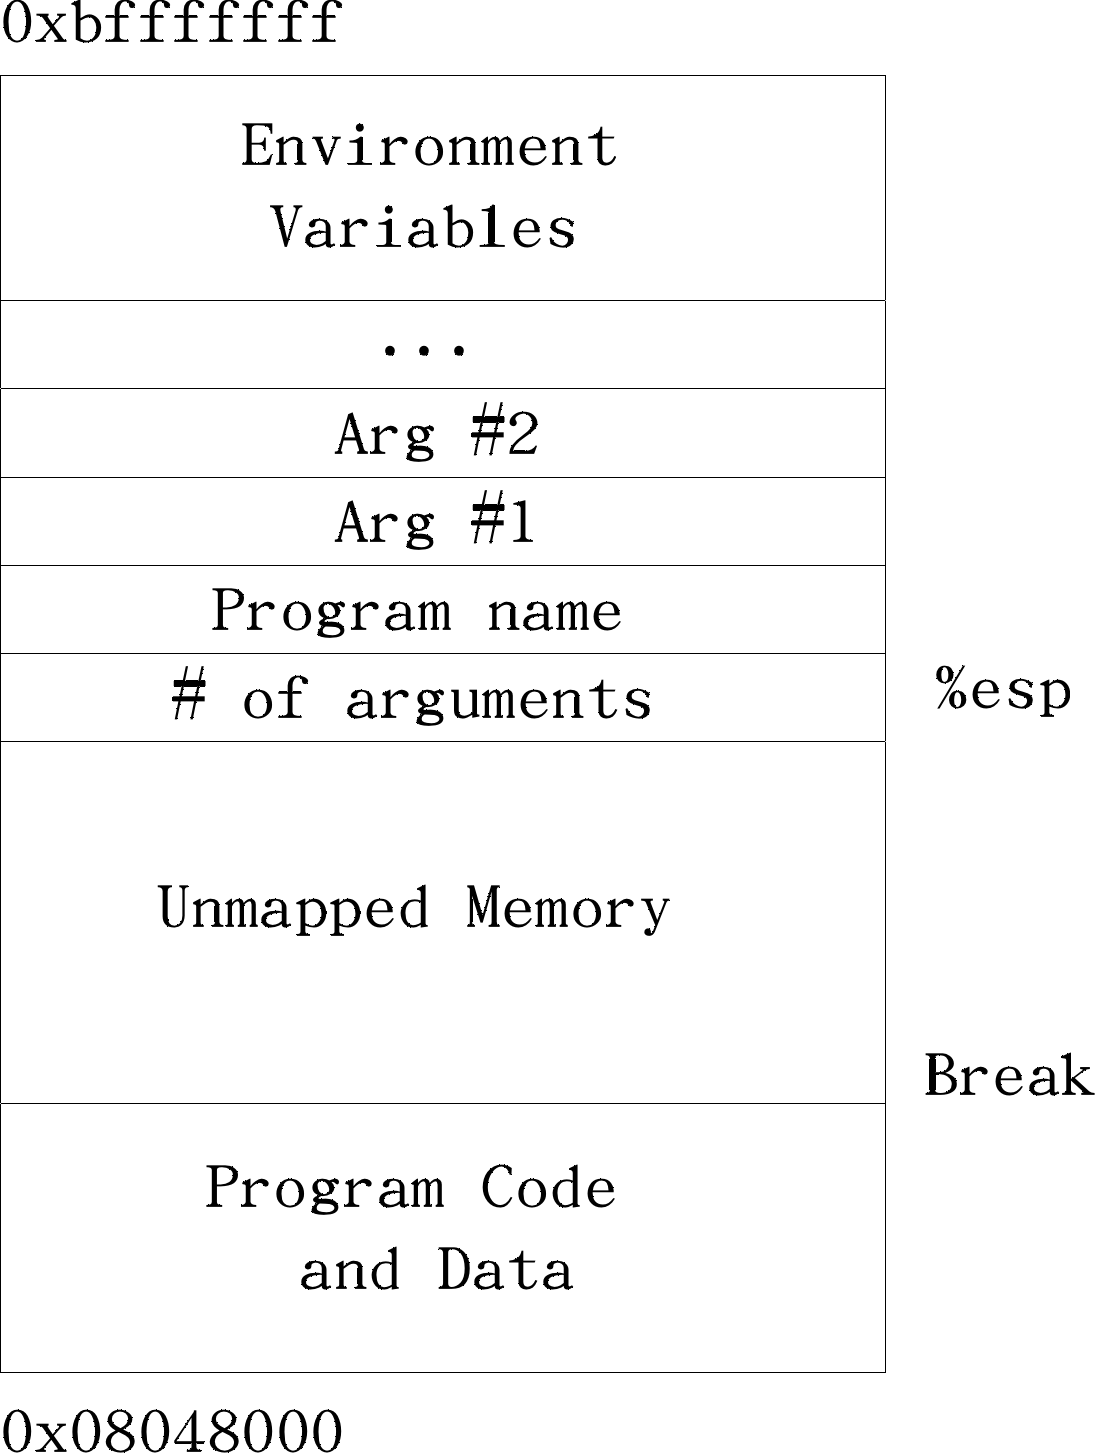
\includegraphics[width=\textwidth]{memorylayout.png}
\end{figure}

\section{Every Memory Address is a Lie}

So, why does the computer not allow you to access memory in the 
break area?  To answer this question, we will have to delve into
the depths of how your computer really handles memory.  

You may have wondered, since every program gets loaded into the same
place in memory, don't they step on each other, or overwrite each other?
It would seem so.  However, as a program writer, you only access
\emph{virtual memory\index{virtual memory}}.  

\emph{Physical memory\index{physical memory}}
refers to the actual RAM chips inside your computer and what they contain.   It's usually
between 16 and 512 Megabytes on modern computers.  If we talk about a \emph{physical
memory address}, we are talking about where exactly on these
chips a piece of memory is located.  Virtual
memory is the way \emph{your program} thinks about memory.  Before loading
your program, Linux finds an empty physical memory space large enough to
fit your program, and then tells
the processor to pretend that this memory is actually at the address
0x0804800 to load your program into.  Confused yet?  Let me explain further.

Each program gets its own sandbox to play in.  Every program running
on your computer thinks that it was loaded at memory address 0x0804800,
and that its stack starts at 0xbffffff.  When Linux loads a program,
it finds a section of unused memory, and then tells the processor to use
that section of memory as the address 0x0804800 for this program.  The
address that a program believes it uses is called the 
virtual address\index{virtual address},
while the actual address on the chips that it refers to is called
the physical address\index{physical address}.  
The process of assigning virtual addresses to
physical addresses is called 
\emph{mapping\index{mapping}}.  

Earlier we 
talked about the inaccessible memory between the \icode{.bss} and the 
stack, but we didn't talk about why it was there.  The reason is that this
region of virtual memory addresses hasn't been mapped onto 
physical memory addresses.  The mapping process takes up considerable
time and space, so if every possible virtual address of every possible
program were mapped, you would not have enough physical memory to even run one program.  So,
the break is the beginning of the area that contains unmapped memory.  With the
stack, however, Linux will automatically map in memory that is accessed from
stack pushes.

Of course, this is a very simplified view of virtual memory.  The full 
concept is much more advanced.  For example, 
Virtual memory can be mapped to more than just physical memory; it
can be mapped to disk as well.  Swap partitions on Linux allow
Linux's virtual memory system to map memory not only to physical RAM,
but also to disk blocks as well.  For example, let's
say you only have 16 Megabytes of physical memory.  Let's also say that
8 Megabytes are being used by Linux and some basic applications, and you
want to run a program that requires 20 Megabytes of memory.  Can you?  The
answer is yes, but only if you have set up a swap partition.  What
happens is that after all of your remaining 8 Megabytes of physical memory
have been mapped into virtual memory, Linux starts mapping parts of your application's
virtual memory to disk blocks.  So, if you access a "memory" location in your
program, that location may not actually be in memory at all, but on
disk.  As the programmer you won't know the difference, though, because 
it is all handled behind the scenes by Linux.

Now, x86 processors cannot run instructions directly from disk, nor can
they access data directly from disk.  This requires the help of the operating
system.  When you try to access memory that is mapped to disk, the processor
notices that it can't service your memory request directly.  It then asks
Linux to step in.  Linux notices that the memory
is actually on disk.  Therefore, it moves some data that is currently in 
memory onto disk to make room, and then moves the memory being accessed
from the disk back into physical memory.  It then adjusts the processor's
virtual-to-physical memory lookup tables so that it can find the memory in
the new location.  Finally, Linux returns control to the program and restarts
it at the instruction which was trying to access the data in the first place.  
This instruction can now be completed successfully, 
because the memory is now in physical RAM.\footnote{Note that not only 
can Linux have a virtual address map to a different
physical address, it can also move those mappings around as needed.
}

Here is an overview of the way memory accesses are handled under Linux:

\begin{itemize}\item The program tries to load memory from a virtual address. 
\item The processor, using tables supplied by Linux, transforms the virtual memory address into a physical memory address on the fly. 
\item If the processor does not have a physical address listed for the memory address, it sends a request to Linux to load it. 
\item Linux looks at the address.  If it is mapped to a disk location, it continues on to the next step.  Otherwise, it terminates the program with a segmentation fault error. 
\item If there is not enough room to load the memory from disk, Linux will move another part of the program or another program onto disk to make room. 
\item Linux then moves the data into a free physical memory address. 
\item Linux updates the processor's virtual-to-physical memory mapping tables to reflect the changes. 
\item Linux restores control to the program, causing it to re-issue the instruction which caused this process to happen. 
\item The processor can now handle the instruction using the newly-loaded memory and translation tables. 
\end{itemize}

It's a lot of work for the operating system, but it gives the user and the programmer great
flexibility when it comes to memory management.

Now, in order to make the process more efficient,
memory is separated out into groups called \emph{pages\index{pages}}.  When
running Linux on x86 processors, a page is 4096 bytes of memory.
All of the memory mappings are done a page at a time.  Physical memory assignment,
swapping\index{swapping}, mapping, etc. are all done to memory pages\index{memory pages} instead of individual memory
addresses.  What this means to you as a programmer
is that whenever you are programming, you should try to keep most memory accesses within
the same basic range of memory, so you will only need a page or two of memory at
a time.  Otherwise, Linux may have to keep moving pages on and off of disk to 
satisfy your memory needs. Disk access is slow, so this can really slow down your program. 

Sometimes so many programs can be loaded that there is hardly enough physical
memory for them.  They wind up spending more time just swapping memory on and off of disk
than they do actually processing it.  This leads to a condition called 
\emph{swap death\index{swap death}}
which leads to your system being unresponsive and unproductive.  It's usually
usually recoverable if you start terminating your memory-hungry programs, but it's a pain.

\begin{sidebar}[Resident Set Size]
The amount of memory that your program currently has in physical memory is called its
resident set size\index{resident set size}, and
can be viewed by using the program \icode{top}.  The resident set size
is listed under the column labelled "RSS".
\end{sidebar}

\section{Getting More Memory}
\label{dynamicmemory}

We now know that Linux maps all of our virtual memory into physical memory or
swap.  If you try to access a piece of virtual memory\index{virtual memory} 
that hasn't been mapped yet,
it triggers an error known as a segmentation fault, which will terminate your 
program.  The program break point, if you remember, is the last valid address you
can use.  Now, this is all great if you know beforehand how much storage you will
need.  You can just add all the memory you need to your \icode{.data}
or \icode{.bss} sections, and it will
all be there.  However, let's say you don't know how much memory you will need.  For example,
with a text editor, you don't know how long the person's file will be.  You could try
to find a maximum file size, and just tell the user that they can't go beyond that, but
that's a waste if the file is small.  Therefore Linux has a facility to move the break point
to accomodate an application's memory needs.

If you need more memory, you can just tell Linux where you want the new break point
to be, and Linux will map all the memory you need between the current and new break
point, and then move the break point to the spot you specify.  That memory is now
available for your program to use.  The
way we tell Linux to move the break point is through the 
\icode{brk\index{brk}} 
system call.  The \icode{brk} system call is call number
45 (which will be in {\eaxReg}).  {\ebxReg} should be loaded with the requested breakpoint.  
Then you call \icode{int \$0x80} to signal Linux to do its work.  
After mapping in your memory, Linux will return the new break point in {\eaxReg}.
The new break point might actually be larger
than what you asked for, because Linux rounds up to the nearest page.  If there is
not enough physical memory or swap to fulfill your request, Linux will return a zero
in {\eaxReg}.  Also, if you call \icode{brk} with a zero in {\ebxReg}, it will
simply return the last usable memory address.

 

The problem with this method is keeping track of the memory we request.  Let's say I need to
move the break to have room to load a file, and then need to move a break again to
load another file.  Let's say I then get rid of the first file.  You now have
a giant gap in memory that's mapped, but that you aren't using.  If you continue to 
move the break in this way for each file you load, you can easily run out of memory.  
So, what is needed is a \emph{memory manager\index{memory manager}}.  

A memory manager is a set of routines that takes care of the dirty work of getting
your program memory for you.  Most memory managers have two basic functions - 
\icode{allocate} and \icode{deallocate}.\footnote{The function 
names usually aren't \icode{allocate} and \icode{deallocate}, but
the functionality will be the same.  In the C programming language, for example, they
are named \icode{malloc} and \icode{free}.}
Whenever you need a certain amount of memory, you can simply tell \icode{allocate}
how much you need, and it will give you back an address to the memory.  
When you're done with it, you tell \icode{deallocate}
that you are through with it.  \icode{allocate} will then be able to reuse the
memory.  This pattern of memory management is called \emph{dynamic memory allocation\index{dynamic memory allocation}}.  
This minimizes the number of "holes" in your memory, making sure that you
are making the best use of it you can.
The pool of memory used by memory managers
is commonly referred to as 
\emph{the heap\index{heap}}.

The way memory managers work is that they keep track of where the system break is, and
where the memory that you have allocated is.  
They mark each block of memory in the heap as
being used or unused.  When you request memory, the memory manager checks to see if there
are any unused blocks of the appropriate size.  If not, it calls the \icode{brk}
system call to request more memory.  When you free memory it marks the block as unused
so that future requests can retrieve it.  In the next section we will look at building
our own memory manager.

\section{A Simple Memory Manager}

Here I will show you a simple memory manager.  It is very primitive but it shows the 
principles quite well.
As usual, I will give you the program first for you to look through.  Afterwards will follow
an in-depth explanation.  It looks long, but it is mostly comments.

\begin{simpletyping}
\lstinputlisting{alloc.s}
\end{simpletyping}

The first thing to notice is that there is no \icode{\_start} symbol.  The reason
is that this is just a set of functions.  A memory manager by itself is not a full 
program - it doesn't do anything.  It is simply a utility to be used by other programs.

To assemble the program, do the following:

\begin{simpletyping}
\begin{lstlisting}
as alloc.s -o alloc.o
\end{lstlisting}
\end{simpletyping}

Okay, now let's look at the code.

\section{Variables and Constants}

At the beginning of the program, we have two locations set up:

\begin{simpletyping}
\begin{lstlisting}
heap\_begin:
	.long 0

current\_break:
	.long 0
\end{lstlisting}
\end{simpletyping}

Remember, the section of memory being managed is commonly referred to as
the \emph{heap\index{heap}}. 
When we assemble the program, we have no idea where the beginning of the heap is, nor 
where the current break\index{current break} 
is.  Therefore, we reserve space for their addresses, but just fill them with a 0 for the
time being.  

Next we have a set of constants to define the structure of the heap.  The way this
memory manager works is that before each region of memory allocated, we will have a 
short record describing the memory.
This record has a word reserved for the available flag and a word for the region's size.
The actual memory allocated immediately follows this record.  The available flag is used
to mark whether this region is available for allocations, or if it is currently in
use.  The size field lets us know both whether or not this region is big enough for
an allocation request, as well as the location of the next memory region.
The following constants describe this record:

\begin{simpletyping}
\begin{lstlisting}
	.equ HEADER\_SIZE, 8
	.equ HDR\_AVAIL\_OFFSET, 0
	.equ HDR\_SIZE\_OFFSET, 4
\end{lstlisting}
\end{simpletyping}

This says that the header is 8 bytes total, the available flag is offset 0 bytes from the 
beginning, and the size field is offset 4 bytes from the 
beginning.  If we are careful to always use these constants,
then we protect ourselves from having to do too much work if we later decide to add more
information to the header.

The values that we will use for our \icode{available} field are either 0 for
unavailable, or 1 for available.  To make this easier to read, we have the following definitions:

\begin{simpletyping}
\begin{lstlisting}
	.equ UNAVAILABLE, 0
	.equ AVAILABLE, 1
\end{lstlisting}
\end{simpletyping}

Finally, we have our Linux system call definitions:

\begin{simpletyping}
\begin{lstlisting}
	.equ BRK, 45
	.equ LINUX\_SYSCALL, 0x80
\end{lstlisting}
\end{simpletyping}

\section{The \icode{allocate\_init} function}

Okay, this is a simple function.  All it does is set up the \icode{heap\_begin} and
\icode{current\_break} variables we discussed earlier.  So, if you remember the
discussion earlier, the current break can be found using the 
\icode{brk\index{brk}} system call.  
So, the function starts like this:

\begin{simpletyping}
\begin{lstlisting}
	pushl {\ebpBare}
	movl  {\espBare}, {\ebpBare}

	movl  \$SYS\_BRK, {\eaxBare}
	movl  \$0,  {\ebxBare}
	int   \$LINUX\_SYSCALL
\end{lstlisting}
\end{simpletyping}

Anyway, after \icode{int \$LINUX\_SYSCALL}, 
\icode{{\eaxBare}} holds the last valid address.  
We actually want the first invalid address instead of the last valid address, so we just increment \icode{{\eaxBare}}.  Then
we move that value to the \icode{heap\_begin} and \icode{current\_break}
locations.  
Then we leave the function.  The code looks like this:

\begin{simpletyping}
\begin{lstlisting}
	incl  {\eaxBare}
	movl  {\eaxBare}, current\_break
	movl  {\eaxBare}, heap\_begin
	movl  {\ebpBare}, {\espBare}
	popl  {\ebpBare}
	ret
\end{lstlisting}
\end{simpletyping}

The heap consists of the memory between \icode{heap\_begin} and
\icode{current\_break}, so this says that we start off with a heap of zero bytes.
Our \icode{allocate} function will then extend the heap as much as it needs to
when it is called.

\section{The \icode{allocate} function}

This is the doozy function.  Let's start by looking at an outline of the function:

\begin{enumerate}
\item Start at the beginning of the heap. 
\item Check to see if we're at the end of the heap. 
\item If we are at the end of the heap, grab the memory we need from Linux, mark it
as "unavailable" and return it.  If Linux won't give us any more, return a 0. 
\item If the current memory region is marked "unavailable", go to the next one, and go
back to step 2. 
\item If the current memory region is too small to hold the requested amount of space,
go back to step 2. 
\item If the memory region is available and large enough, mark it as "unavailable" and
return it. 
\end{enumerate}

Now, look back through the code with this in mind.  Be sure to read the comments so you'll know 
which register holds which value.  

Now that you've looked back through the code, let's examine it one line at a time.  We start
off like this:

\begin{simpletyping}
\begin{lstlisting}
	pushl {\ebpBare}
	movl  {\espBare}, {\ebpBare}
	movl  ST\_MEM\_SIZE({\ebpBare}), {\ecxBare}
	movl  heap\_begin, {\eaxBare}
	movl  current\_break, {\ebxBare}
\end{lstlisting}
\end{simpletyping}

This part initializes all of our registers.  The first two lines are standard function
stuff.  The next move pulls the size of the memory to allocate off of the stack.  This is
our only function parameter.   After that, it moves the beginning heap address and the 
end of the heap into registers.  I am now ready to do processing.

The next section is marked \icode{alloc\_loop\_begin}.  In this loop
we are going to examine memory regions until we either find an open memory region or 
determine that we need more memory.  Our first instructions check to see if we need more memory:

\begin{simpletyping}
\begin{lstlisting}
	cmpl {\ebxBare}, {\eaxBare}
	je   move\_break
\end{lstlisting}
\end{simpletyping}

{\eaxReg} holds the current memory region being examined and {\ebxReg}
holds the location past the end of the heap.  Therefore if the next region to be
examined is past the end of the heap, it means we need more 
memory to allocate a region of this size.  
Let's skip down to \icode{move\_break} and
see what happens there:

\begin{simpletyping}
\begin{lstlisting}
move\_break:
	addl  \$HEADER\_SIZE, {\ebxBare}
	addl  {\ecxBare}, {\ebxBare}
	pushl {\eaxBare}
	pushl {\ecxBare}
	pushl {\ebxBare}
	movl  \$SYS\_BRK, {\eaxBare}
	int   \$LINUX\_SYSCALL
\end{lstlisting}
\end{simpletyping}

When we reach this point in the code, {\ebxReg} holds where we want the next
region of memory to be.    
So, we add our header size and region size to {\ebxReg}, and that's where we want the system break 
to be.  We then push all the registers we want to save on the stack, and call the 
\icode{brk} system call. After that we check for errors:

\begin{simpletyping}
\begin{lstlisting}
	cmpl  \$0, {\eaxBare}
	je    error
\end{lstlisting}
\end{simpletyping}

If there were no errors we pop the registers back off the stack, mark the memory as 
unavailable, record the size of the memory, and make sure {\eaxReg} points to the start of usable
memory (which is \emph{after} the header).

\begin{simpletyping}
\begin{lstlisting}
	popl  {\ebxBare}
	popl  {\ecxBare}
	popl  {\eaxBare}
	movl  \$UNAVAILABLE, HDR\_AVAIL\_OFFSET({\eaxBare})
	movl  {\ecxBare}, HDR\_SIZE\_OFFSET({\eaxBare})
	addl  \$HEADER\_SIZE, {\eaxBare}
\end{lstlisting}
\end{simpletyping}

Then we store the new program break and return the pointer to the allocated memory.

\begin{simpletyping}
\begin{lstlisting}
	movl  {\ebxBare}, current\_break
	movl  {\ebpBare}, {\espBare}
	popl  {\ebpBare}
	ret
\end{lstlisting}
\end{simpletyping}

The \icode{error} code just returns 0 in {\eaxReg}, so we won't 
discuss it.

Let's go back look at the rest of the loop.  What happens if the current memory being 
looked at isn't past the end of the heap?  Well, let's look.

\begin{simpletyping}
\begin{lstlisting}
	movl HDR\_SIZE\_OFFSET({\eaxBare}), {\edxBare}
	cmpl \$UNAVAILABLE, HDR\_AVAIL\_OFFSET({\eaxBare})
	je   next\_location
\end{lstlisting}
\end{simpletyping}

This first grabs the size of the memory region and puts it in {\edxReg}.
Then it looks at the available flag to see if it is set to \icode{UNAVAILABLE}.
If so, that means that memory region is in use, so we'll have to skip over it.  So, if
the available flag is set to \icode{UNAVAILABLE}, you go to the code
labeled \icode{next\_location}.  If the available flag is set to
\icode{AVAILABLE}, then we keep on going.  

Let's say that the space was available, and so we keep going.  Then we check to
see if this space is big enough to hold the requested amount of memory.  The size of
this region is being held in {\edxReg}, so we do this:

\begin{simpletyping}
\begin{lstlisting}
	cmpl  {\edxBare}, {\ecxBare}
	jle   allocate\_here
\end{lstlisting}
\end{simpletyping}

If the requested size is less than or equal to the current region's size, we
can use this block.  It doesn't matter if the current region is larger than requested,
because the extra space will just be unused.  So, let's jump down to 
\icode{allocate\_here} and see what happens:

\begin{simpletyping}
\begin{lstlisting}
	movl  \$UNAVAILABLE, HDR\_AVAIL\_OFFSET({\eaxBare})
	addl  \$HEADER\_SIZE, {\eaxBare}
	movl  {\ebpBare}, {\espBare}
	popl  {\ebpBare}
	ret
\end{lstlisting}
\end{simpletyping}

It marks the memory as being unavailable.  Then it moves the pointer {\eaxReg} past the header,
and uses it as the return value for the function.  Remember, the person using this
function doesn't need to even know about our memory header record.  They just need
a pointer to usable memory. 

Okay, so let's say the region wasn't big enough.  What then?  Well, we would then
be at the code labeled \icode{next\_location}.  This section of code
is used any time that we figure out that
the current memory region won't work for allocating memory.  All it does is
advance {\eaxReg} to the next possible memory region, and goes back
to the beginning of the loop.   Remember that {\edxReg} is holding
the size of the current memory region, and \icode{HEADER\_SIZE} is the symbol
for the size of the memory region's header.  So this code will move us to the next
memory region:

\begin{simpletyping}
\begin{lstlisting}
	addl  \$HEADER\_SIZE, {\eaxBare}
	addl  {\edxBare}, {\eaxBare}
	jmp   alloc\_loop\_begin
\end{lstlisting}
\end{simpletyping}

And now the function runs another loop.

Whenever you have a loop, you must make sure that it will \emph{always} 
end.  The best way to do that is to examine all of the possibilities, and make sure that
all of them eventually lead to the loop ending.  In our case, we have the following 
possibilities:

\begin{itemize}
\item We will reach the end of the heap 
\item We will find a memory region that's available and large enough 
\item We will go to the next location 
\end{itemize}

The first two items are conditions that will cause the loop to end.  The third one
will keep it going.  However, even if we never find an open region, 
we will eventually reach the end of the heap, because it is a finite size.  Therefore, we know
that no matter which condition is true, the loop has to eventually hit a terminating condition.

\section{The \icode{deallocate} function}

The \icode{deallocate} function is much easier than the 
\icode{allocate} one.
That's because it doesn't have to do any searching at all.  It can just mark
the current memory region as \icode{AVAILABLE}, and \icode{allocate}
will find it next time it is called.   So we have:

\begin{simpletyping}
\begin{lstlisting}
	movl  ST\_MEMORY\_SEG({\espBare}), {\eaxBare}
	subl  \$HEADER\_SIZE, {\eaxBare}
	movl  \$AVAILABLE, HDR\_AVAIL\_OFFSET({\eaxBare})
	ret
\end{lstlisting}
\end{simpletyping}

In this function, we don't have to save {\ebpRegIdx} or {\espRegIdx}
since we're not changing them, nor do we have to restore them at the end.  All we're
doing is reading the address of the memory region from the stack, backing up to the
beginning of the header, and marking the region as available.  This function has no
return value, so we don't care what we leave in {\eaxReg}.

\section{Performance Issues and Other Problems}

Our simplistic memory manager is not really useful for anything more than an academic exercise.
This section looks at the problems with such a simplistic allocator.

The biggest problem here is speed.  Now, if there are only a few allocations made,
then speed won't be a big issue.  But think about what happens if you make a thousand
allocations.  On allocation number 1000, you have to search through 999 memory regions
to find that you have to request more memory.  As you can see, that's getting pretty
slow.  In addition, remember that Linux can keep pages of memory on disk instead of in
memory.  So, since you have to go through every piece of memory your program's memory, that means that Linux
has to load every part of memory that's currently on disk to check to see if it is available.  
You can see how this could get really, really slow.\footnote{This is why adding more
memory to your computer makes it run faster.  The more memory your computer has, the
less it puts on disk, so it doesn't have to always be interrupting your programs to
retreive pages off the disk.}  This method is said to run in 
\emph{linear} time, which means that every element you have to
manage makes your program take longer.   A program that runs in \emph{constant}
time takes the same amount of time no matter how many elements you are managing.
Take the \icode{deallocate} function, for instance.  It only runs 4 instructions,
no matter how many elements we are managing, or where they are in memory.  In fact, although
our \icode{allocate} function is one of the slowest of all memory managers,
the \icode{deallocate} function is one of the fastest.  

Another performance problem is the number of times we're calling the \icode{brk}
system call.
System calls take a long time.  They aren't like functions, because the processor has
to switch modes.  Your program isn't allowed to map itself memory, but the Linux kernel is.  
So, the processor has to switch into \emph{kernel mode\index{kernel mode}}, then Linux maps the
memory, and then switches back to \emph{user mode\index{user mode}} for your application to continue running.  
This is also called
a \emph{context switch\index{context switch}}.  
Context switches are relatively slow on x86 processors.
Generally, you should avoid calling the kernel unless you really need to.  

Another problem that we have is that we aren't recording where Linux actually sets the break.  
Previously we mentioned that Linux might actually set the break past where we requested
it.  In this program, we don't even look at where Linux actually sets the break - we just
assume it sets it where we requested.  That's not really a bug, but it will lead to 
unnecessary \icode{brk} system calls when we already have the memory mapped in.

Another problem we have is that if we are looking for a 5-byte region of memory, and
the first open one we come to is 1000 bytes, we will simply mark the whole thing
as allocated and return it.  This leaves 995 bytes of unused, but allocated, memory.
It would be nice in such situations to break it apart so the other 995 bytes can be
used later.  It would also be nice to combine consecutive free spaces when looking
for large allocations.

\section{Using our Allocator}

The programs we do in this book aren't complicated enough to necessitate a memory
manager.  Therefore, we will just use our memory manager to allocate a buffer
for one of our file reading/writing programs instead of assigning it in the 
\icode{.bss}.

The program we will demonstrate this on is \icodefilename{read-records.s} from
\autoref{records}.  This program uses a buffer named \icode{record\_buffer}
to handle its input/output needs.  We will simply change this from being a buffer defined
in \icode{.bss} to being a pointer to a dynamically-allocated buffer using
our memory manager.  You will need to have the code from that program handy as we will
only be discussing the changes in this section.

The first change we need to make is in the declaration.  Currently it looks like this:

\begin{simpletyping}
\begin{lstlisting}
	.section .bss
	.lcomm, record\_buffer, RECORD\_SIZE
\end{lstlisting}
\end{simpletyping}

It would be a misnomer to keep the same name, since we are switching it from being an
actual buffer to being a pointer to a buffer.  In addition, it now only needs to be
one word big (enough to hold a pointer).  The new declaration will stay in the 
\icode{.data} section and look like this:

\begin{simpletyping}
\begin{lstlisting}
record\_buffer\_ptr:
	.long 0
\end{lstlisting}
\end{simpletyping}

Our next change is we need to initialize our memory manager immediately after 
we start our program.  Therefore, right after the stack is set up, the following
call needs to be added:

\begin{simpletyping}
\begin{lstlisting}
	call allocate\_init
\end{lstlisting}
\end{simpletyping}

After that, the memory manager is ready to start servicing memory allocation requests.
We need to allocate enough memory to hold these records that we are reading.  Therefore,
we will call \icode{allocate} to allocate this memory, and then save the
pointer it returns into \icode{record\_buffer\_ptr}.  Like this:

\begin{simpletyping}
\begin{lstlisting}
	pushl \$RECORD\_SIZE
	call  allocate
	movl  {\eaxBare}, record\_buffer\_ptr
\end{lstlisting}
\end{simpletyping}

Now, when we make the call to \icode{read\_record}, it is expecting a pointer.
In the old code, the pointer was the immediate-mode reference to 
\icode{record\_buffer}.  Now, \icode{record\_buffer\_ptr} just holds
the pointer rather than the buffer itself.  Therefore, we must do a direct mode load
to get the value in \icode{record\_buffer\_ptr}.  We need to remove this line:

\begin{simpletyping}
\begin{lstlisting}
pushl \$record\_buffer
\end{lstlisting}
\end{simpletyping}

And put this line in its place:

\begin{simpletyping}
\begin{lstlisting}
pushl record\_buffer\_ptr
\end{lstlisting}
\end{simpletyping}

The next change comes when we are trying to find the address of the 
firstname field of our record.  In the old code, it was 
\icode{\$RECORD\_FIRSTNAME + record\_buffer}.  However, that
only works because it is a constant offset from a constant address.
In the new code, it is the offset of an address stored in 
\icode{record\_buffer\_ptr}.  To get that value, we will need
to move the pointer into a register, and then add \icode{\$RECORD\_FIRSTNAME}
to it to get the pointer.  So where we have the following code:

\begin{simpletyping}
\begin{lstlisting}
	pushl \$RECORD\_FIRSTNAME + record\_buffer
\end{lstlisting}
\end{simpletyping}

We need to replace it with this:

\begin{simpletyping}
\begin{lstlisting}
	movl  record\_buffer\_ptr, {\eaxBare}
	addl  \$RECORD\_FIRSTNAME, {\eaxBare}
	pushl {\eaxBare}
\end{lstlisting}
\end{simpletyping}

Similarly, we need to change the line that says

\begin{simpletyping}
\begin{lstlisting}
	movl  \$RECORD\_FIRSTNAME + record\_buffer, {\ecxBare}
\end{lstlisting}
\end{simpletyping}

so that it reads like this:

\begin{simpletyping}
\begin{lstlisting}
	movl  record\_buffer\_ptr, {\ecxBare}
	addl  \$RECORD\_FIRSTNAME, {\ecxBare}
\end{lstlisting}
\end{simpletyping}

Finally, one change that we need to make is to deallocate the memory once
we are done with it (in this program it's not necessary, but it's a good 
practice anyway).  To do that, we just send \icode{record\_buffer\_ptr}
to the \icode{deallocate} function right before exitting:

\begin{simpletyping}
\begin{lstlisting}
	pushl record\_buffer\_ptr
	call  deallocate
\end{lstlisting}
\end{simpletyping}

Now you can build your program with the following commands:

\begin{simpletyping}
\begin{lstlisting}
as read-records.s -o read-records.o
ld alloc.o read-record.o read-records.o write-newline.o count-chars.o -o read-records
\end{lstlisting}
\end{simpletyping}

You can then run your program by doing \icode{./read-records}.

The uses of dynamic memory allocation may not be apparent to you at this point, but as
you go from academic exercises to real-life programs you will use it continually.

\section{More Information}

More information on memory handling in Linux and other operating systems can be
found at the following locations:

\begin{itemize}\item More information about the memory layout of Linux programs can be found in Konstantin Boldyshev's document, "Startup state of a Linux/i386 ELF binary", available at http://linuxassembly.org/startup.html 
\item A good overview of virtual memory in many different systems is available at http://cne.gmu.edu/modules/vm/ 
\item Several in-depth articles on Linux's virtual memory subsystem is available at http://www.nongnu.org/lkdp/files.html 
\item Doug Lea has written up a description of his popular memory allocator at http://gee.cs.oswego.edu/dl/html/malloc.html 
\item A paper on the 4.4 BSD memory allocator is available at http://docs.freebsd.org/44doc/papers/malloc.html 
\end{itemize}

\section{Review}

\section{Know the Concepts}

\begin{itemize}\item Describe the layout of memory when a Linux program starts. 
\item What is the heap? 
\item What is the current break? 
\item Which direction does the stack grow in? 
\item Which direction does the heap grow in? 
\item What happens when you access unmapped memory? 
\item How does the operating system prevent processes from writing over each other's memory? 
\item Describe the process that occurs if a piece of memory you are using is currently residing on disk? 
\item Why do you need an allocator? 
\end{itemize}

\section{Use the Concepts}

\begin{itemize}\item Modify the memory manager so that it calls \icode{allocate\_init} automatically if it hasn't been initialized. 
\item Modify the memory manager so that if the requested size of memory is smaller than the region chosen, it will break up the region into multiple parts.  Be sure to take into account the size of the new header record when you do this. 
\item Modify one of your programs that uses buffers to use the memory manager to get buffer memory rather than using the \icode{.bss}. 
\end{itemize}

\section{Going Further}

\begin{itemize}\item Research \emph{garbage collection}.  What advantages and disadvantages does this have over the style of memory management used here? 
\item Research \emph{reference counting}.  What advantages and disadvantages does this have over the style of memory management used here? 
\item Change the name of the functions to \icode{malloc} and \icode{free}, and build them into a shared library.  Use \icode{LD\_PRELOAD} to force them to be used as your memory manager instead of the default one.  Add some \icode{write} system calls to STDOUT to verify that your memory manager is being used instead of the default one. 
\end{itemize}


\chapter{Counting Like a Computer}
\label{countingchapter}

%  FIXME - See Dominique note 

% 
% 
% Copyright 2002 Jonathan Bartlett
% 
% Permission is granted to copy, distribute and/or modify this
% document under the terms of the GNU Free Documentation License,
% Version 1.1 or any later version published by the Free Software
% Foundation; with no Invariant Sections, with no Front-Cover Texts,
% and with no Back-Cover Texts.  A copy of the license is included in fdl.xml
% 

\section{Counting}

\section{Counting Like a Human}

In many ways, computers count just like humans.  So, before we
start learning how computers count, let's take a deeper look at
how we count.

How many fingers do you have?  No, it's not a trick question.
Humans (normally) have ten fingers.  Why is that significant?
Look at our numbering system.  At what point does a one-digit
number become a two-digit number?  That's right, at ten.  Humans
count and do math using a base ten numbering system.  Base ten
means that we group everything in tens.  Let's say we're counting
sheep.  1, 2, 3, 4, 5, 6, 7, 8, 9, 10.  Why did we all of a sudden
now have two digits, and re-use the 1?  That's because we're grouping
our numbers by ten, and we have 1 group of ten sheep.  Okay, let's
go to the next number 11.  That means we have 1 group of ten sheep,
and 1 sheep left ungrouped.  So we continue - 12, 13, 14, 15, 16, 17,
18, 19, 20.  Now we have 2 groups of ten.  21 - 2 groups of ten, and
1 sheep ungrouped.  22 - 2 groups of ten, and 2 sheep ungrouped.   So,
let's say we keep counting, and get to 97, 98, 99, and 100.  Look, it
happened again!  What happens at 100?  We now have ten groups of ten.
At 101 we have ten groups of ten, and 1 ungrouped sheep.  So we can
look at any number like this.  If we counted 60879 sheep, that would
mean that we had 6 groups of ten groups of ten groups of ten groups of ten,
0 groups of ten groups of ten groups of ten, 8 groups of ten groups of ten,
7 groups of ten, and 9 sheep left ungrouped.  

So, is there anything significant about grouping things by ten?  No!  It's
just that grouping by ten is how we've always done it, because we have
ten fingers.  We could have grouped at nine or at eleven (in which case
we would have had to make up a new symbol).  The only difference between
the different groupings of numbers is that we have to re-learn our
multiplication, addition, subtraction, and division tables for each
grouping.  The rules
haven't changed, just the way we represent them.  Also, some of our
tricks that we learned don't always apply, either.  For example, let's
say we grouped by nine instead of ten.  Moving the decimal point one
digit to the right no longer multiplies by ten, it now multiplies by nine.
In base nine, 500 is only nine times as large as 50.

\section{Counting Like a Computer}

The question is, how many fingers does the computer have to count with?
The computer only has two fingers.  So that means all of the groups are 
groups of two.  So, let's count in binary - 0 (zero), 1 (one), 10 (two - 
one group of two), 11 (three - one group of two and one left over), 
100 (four - two groups of two), 101 (five - two groups of two and one left 
over), 110 (six - two groups of two and one group of two), and so on.  
In base two, moving the decimal one digit to the right multiplies by two, and 
moving it to the left divides by two.  Base two\index{base two} is also referred to
as binary.

The nice thing about base two is that the basic math tables are very
short.  In base ten, the multiplication tables are ten columns wide,
and ten columns tall.  In base two, it is very simple:

\begin{simpletyping}
\begin{lstlisting}
%  NOTE - these need to be converted to tables 

Table of binary addition

+ |  0  |  1  
--+-----+-----
0 |  0  |  0  
--+-----+-----
1 |  1  | 10  

Table of binary multiplication

* |  0  |  1
--+-----+-----
0 |  0  |  0
--+-----+-----
1 |  0  |  1

\end{lstlisting}
\end{simpletyping}

So, let's add the numbers 10010101 with 1100101:

\begin{simpletyping}
\begin{lstlisting}
   10010101
+   1100101
-----------
   11111010
\end{lstlisting}
\end{simpletyping}

Now, let's multiply them:

\begin{simpletyping}
\begin{lstlisting}

        10010101
     *   1100101
     -----------
        10010101
       00000000
      10010101
     00000000
    00000000
   10010101
  10010101
 ---------------
  11101011001001
\end{lstlisting}
\end{simpletyping}

\section{Conversions Between Binary and Decimal}

Let's learn how to convert numbers from binary\index{binary} (base two\index{base two}) to 
decimal\index{decimal} (base ten\index{base ten}).  This is actually a rather simple process.
If you remember, each digit\index{digit} stands for some grouping of two.  So,
we just need to add up what each digit represents, and we will have
a decimal number.  Take the binary number 10010101.  To find out
what it is in decimal, we take it apart like this:

\begin{simpletyping}
\begin{lstlisting}
     1    0    0    1    0    1    0    1
     |    |    |    |    |    |    |    |
     |    |    |    |    |    |    |    Individual units (2\textasciicircum0)
     |    |    |    |    |    |    0 groups of 2 (2\textasciicircum1)
     |    |    |    |    |    1 group of 4 (2\textasciicircum2)
     |    |    |    |    0 groups of 8 (2\textasciicircum3)
     |    |    |    1 group of 16 (2\textasciicircum4)
     |    |    0 groups of 32 (2\textasciicircum5)
     |    0 groups of 64 (2\textasciicircum6)
     1 group of 128 (2\textasciicircum7)
\end{lstlisting}
\end{simpletyping}

and then we add all of the pieces together, like this:

\begin{simpletyping}
\begin{lstlisting}
1*128 + 0*64 + 0*32 + 1*16 + 0*8 + 1*4 + 0*2 + 1*1 =
128 + 16 + 4 + 1 = 
149
\end{lstlisting}
\end{simpletyping}

So 10010101 in binary is 149 in decimal.  Let's look at 1100101.  It
can be written as

\begin{simpletyping}
\begin{lstlisting}
1*64 + 1*32 + 0 * 16 + 0*8 + 1*4 + 0*2 + 1*1 =
64 + 32 + 4 + 1 =
101
\end{lstlisting}
\end{simpletyping}

So we see that 1100101 in binary is 101 in decimal.  Let's look at
one more number, 11101011001001.  You can convert it to decimal by doing

\begin{simpletyping}
\begin{lstlisting}
1*8192 + 1*4096 + 1*2048 + 0*1024 + 1*512 + 0*256 
       + 1*128 + 1*64 + 0*32 + 0*16 + 1*8 + 0*4 
       + 0*2 + 1*1 =

8192 + 4096 + 2048 + 512 + 128 + 64 + 8 + 1 =

15049
\end{lstlisting}
\end{simpletyping}

Now, if you've been paying attention, you have noticed that the numbers
we just converted are the same ones we used to multiply with earlier.
So, let's check our results: 101 * 149 = 15049.  It worked!

Now let's look at going from decimal\index{decimal} back to binary\index{binary}.  In order to do
the conversion, you have to \emph{divide} the number
into groups of two.  So, let's say you had the number 17.  If you
divide it by two, you get 8 with 1 left over.  So that means there are
8 groups of two, and 1 ungrouped.  That means that the rightmost digit
will be 1.  Now, we have the rigtmost digit figured out, and 8 groups
of 2 left over.  Now, let's see how many groups of two groups of two we 
have, by dividing 8 by 2.  We get 4, with nothing left over.  That
means that all groups two can be further divided into more groups of
two.  So, we have 0 groups of only two.  So the next digit to the
left is 0.  So, we divide 4 by 2 and get two, with 0 left over, so
the next digit is 0.  Then, we divide 2 by 2 and get 1, with 0 left over.
So the next digit is 0.  Finally, we divide 1 by 2 and get 0 with 1
left over, so the next digit to the left is 1.  Now, there's nothing
left, so we're done.  So, the number we wound up with is 10001.

Previously, we converted to binary 11101011001001 to decimal 15049.  Let's
do the reverse to make sure that we did it right:

\begin{simpletyping}
\begin{lstlisting}
15049 / 2 = 7524    Remaining 1
7524 / 2 = 3762     Remaining 0
3762 / 2 = 1881     Remaining 0
1881 / 2 = 940      Remaining 1
940 / 2 = 470       Remaining 0
470 / 2 = 235       Remaining 0
235 / 2 = 117       Remaining 1
117 / 2 = 58        Remaining 1
58 / 2 = 29         Remaining 0
29 / 2 = 14         Remaining 1
14 / 2 = 7          Remaining 0
7 / 2 = 3           Remaining 1
3 / 2 = 1           Remaining 1
1 / 2 = 0           Remaining 1
\end{lstlisting}
\end{simpletyping}

Then, we put the remaining numbers back together, and we have the original
number!  Remember the first division remainder goes to the far right, so
from the bottom up you have 11101011001001.

Each digit in a binary number is called a \emph{bit\index{bits}}, which
stands for \emph{binary digit\index{binary digit}}.  Remember, computers divide up
their memory into storage locations called bytes\index{bytes}.  Each storage location on an x86 processor (and most others) is 8 bits long.  Earlier we said
that a byte can hold any number between 0 and 255.  The reason for this
is that the largest number you can fit into 8 bits is 255.  You can
see this for yourself if you convert binary 11111111 into decimal:

\begin{simpletyping}
\begin{lstlisting}
11111111 =

(1 * 2\textasciicircum7) + (1 * 2\textasciicircum6) + (1 * 2\textasciicircum5) + (1 * 2\textasciicircum4) + (1 * 2\textasciicircum3) 
          + (1 * 2\textasciicircum2) + (1 * 2\textasciicircum1) + (1 * 2\textasciicircum0) = 

128 + 64 + 32 + 16 + 8 + 4 + 2 + 1 =

255
\end{lstlisting}
\end{simpletyping}

The largest number that you can hold in 16 bits is 65535.   The largest
number you can hold in 32 bits is 4294967295 (4 billion).  The largest
number you can hold in 64 bits is 18,446,744,073,709,551,615.  The
largest number you can hold in 128 bits is
340,282,366,920,938,463,463,374,607,431,768,211,456.  Anyway, you
see the picture.  For x86 processors, most of the time you will deal with 4-byte
numbers (32 bits), because that's the size of the registers\index{registers}.

\section{Truth, Falsehood, and Binary Numbers}
\label{truthbinarynumbers}

Now we've seen that the computer stores everything as sequences of
1's and 0's.  Let's look at some other uses of this.  What if, instead
of looking at a sequence of bits\index{bits} as a number, we instead looked at
it as a set of switches\index{switches}.  For example, let's say there are four switches
that control lighting in the house.  We have a switch for outside lights,
a switch for the hallway lights, a switch for the living room lights,
and a switch for the bedroom lights.  We could make a little table
showing which of these were on and off, like so:

\begin{simpletyping}
\begin{lstlisting}
Outside  Hallway  Living Room  Bedroom
  On       Off        On         On
\end{lstlisting}
\end{simpletyping}

It's obvious from looking at this that all of the lights are on except
the hallway ones.  Now, instead of using the words "On" and "Off",
let's use the numbers 1 and 0.  1 will represent on, and 0 will represent
off.  So, we could represent the same information as

\begin{simpletyping}
\begin{lstlisting}
Outside  Hallway  Living Room  Bedroom
   1        0           1         1
\end{lstlisting}
\end{simpletyping}

Now, instead of having labels on the light switches, let's say we just
memorized which position went with which switch.  Then, the same
information could be represented as

\begin{simpletyping}
\begin{lstlisting}
1           0           1         1
\end{lstlisting}
\end{simpletyping}

or as

\begin{simpletyping}
\begin{lstlisting}
1011
\end{lstlisting}
\end{simpletyping}

This is just one of many ways you can use the computers storage locations
to represent more than just numbers.  The computers memory just sees numbers,
but programmers can use these numbers to represent anything their imaginations
can come up with.  They just sometimes have to be creative when figuring out
the best representation.

Not only can you do regular arithmetic with binary numbers, they also have
a few operations of their own, called binary
\index{binary operations} 
or logical operations
\index{logical operations}.  
The standard binary operations are

\begin{itemize}\item AND\index{AND} 
\item OR\index{OR} 
\item NOT\index{NOT} 
\item XOR\index{XOR} 
\end{itemize}

Before we look at examples, I'll describe them for you.
AND takes two bits and returns one bit.  AND will return a 1 only if
both bits are 1, and a 0 otherwise.  For example, 1 AND 1 is 1, but
1 AND 0 is 0, 0 AND 1 is 0, and 0 AND 0 is 0.  

OR takes two bits
and returns one bit.  It will return 1 if either of the original bits
is 1.  For example, 1 OR 1 is 1, 1 OR 0 is one, 0 OR 1 is 1, but 0 OR 0
is 0.

NOT only takes one bit and returns its opposite.  NOT 1 is 0 and
NOT 0 is 1.  

Finally, XOR is like OR, except it returns 0 if both bits
are 1.

Computers can do these operations on whole registers at a time.
For example, if a register has 10100010101010010101101100101010 and
another one has 10001000010101010101010101111010, you can run any of
these operations on the whole registers.  For example, if we were to
AND them, the computer will run from the first bit to the 32nd and run
the AND\index{AND} operation on that bit in both registers.  In this case:

\begin{simpletyping}
\begin{lstlisting}
10100010101010010101101100101010 AND
10001000010101010101010101111010
--------------------------------
10000000000000010101000100101010
\end{lstlisting}
\end{simpletyping}

You'll see that the resulting set of bits only has a one where 
\emph{both} numbers had a one, and in every other position
it has a zero.  Let's look at what an OR\index{OR} looks like:

\begin{simpletyping}
\begin{lstlisting}
10100010101010010101101100101010 OR 
10001000010101010101010101111010
--------------------------------
10101010111111010101111101111010
\end{lstlisting}
\end{simpletyping}

In this case, the resulting number has a 1 where either number has
a 1 in the given position.  Let's look at the NOT\index{NOT} operation:

\begin{simpletyping}
\begin{lstlisting}
NOT 10100010101010010101101100101010
------------------------------------
    01011101010101101010010011010101
\end{lstlisting}
\end{simpletyping}

This just reverses each digit.  Finally, we have XOR\index{XOR}, which is
like an OR, except if \emph{both} digits are 1, it
returns 0.

\begin{simpletyping}
\begin{lstlisting}
10100010101010010101101100101010 XOR 
10001000010101010101010101111010
--------------------------------
00101010111111000000111001010000
\end{lstlisting}
\end{simpletyping}

This is the same two numbers used in the OR operation, so you can 
compare how they work.  Also, if you XOR a number with itself, you 
will always get 0, like this:

\begin{simpletyping}
\begin{lstlisting}
10100010101010010101101100101010 XOR 
10100010101010010101101100101010
--------------------------------
00000000000000000000000000000000
\end{lstlisting}
\end{simpletyping}

These operations are useful for two reasons:

\begin{itemize}\item The computer can do them extremely fast 
\item You can use them to compare many truth values at the same time 
\end{itemize}

You may not have known that different instructions execute at different
speeds.  It's true, they do.  And these operations are the
fastest on most processors.  For example, you saw that XORing a number with 
itself produces 0.  Well, the XOR\index{XOR} operation is faster than the loading operation, so
many programmers use it to load a register\index{register} with zero.  For example, the
code

\begin{simpletyping}
\begin{lstlisting}
	movl  \$0, {\eaxBare}
\end{lstlisting}
\end{simpletyping}

is often replaced by

\begin{simpletyping}
\begin{lstlisting}
	xorl  {\eaxBare}, {\eaxBare}
\end{lstlisting}
\end{simpletyping}

We'll discuss speed more in \autoref{optimizationch}, but I want you
to see how programmers often do tricky things, especially with these
binary operators, to make things fast.  Now let's look at how we
can use these operators to manipulate true\index{true}/false\index{false} values.  Earlier
we discussed how binary numbers can be used to represent any number
of things.  Let's use binary numbers to represent what things my
Dad and I like.  First, let's look at the things I like:

\begin{simpletyping}
\begin{lstlisting}
Food: yes
Heavy Metal Music: yes
Wearing Dressy Clothes: no
Football: yes
\end{lstlisting}
\end{simpletyping}

Now, let's look at what my Dad likes:

\begin{simpletyping}
\begin{lstlisting}
Food: yes
Heavy Metal Music: no
Wearing Dressy Clothes: yes
Football: yes
\end{lstlisting}
\end{simpletyping}

Now, let's use a 1 to say yes we like something, and a 0 to say no we don't.
Now we have:

\begin{simpletyping}
\begin{lstlisting}
Me
Food: 1
Heavy Metal Music: 1
Wearing Dressy Clothes: 0
Football: 1

Dad
Food: 1
Heavy Metal Music: 0
Wearing Dressy Clothes: 1
Football: 1
\end{lstlisting}
\end{simpletyping}

Now, if we just memorize which position each of these are in, we have

\begin{simpletyping}
\begin{lstlisting}
Me
1101

Dad
1011
\end{lstlisting}
\end{simpletyping}

Now, let's see we want to get a list of things both my Dad and I like.
You would use the AND\index{AND} operation.  So

\begin{simpletyping}
\begin{lstlisting}
1101 AND
1011
--------
1001
\end{lstlisting}
\end{simpletyping}

Which translates to

\begin{simpletyping}
\begin{lstlisting}
Things we both like
Food: yes
Heavy Metal Music: no
Wearing Dressy Clothes: no
Football: yes
\end{lstlisting}
\end{simpletyping}

Remember, the computer has no idea what the ones and zeroes represent.
That's your job and your program's job.  If you wrote a program
around this representation your program would at some point examine
each bit and have code to tell the user what it's for (if you asked a computer
what two people agreed on and it answered 1001, it wouldn't be very
useful).  Anyway, let's say we want to know the things that we disagree
on.  For that we would use XOR\index{XOR}, because it will return 1 only if one
or the other is 1, but not both.  So

\begin{simpletyping}
\begin{lstlisting}
1101 XOR
1011
--------
0110
\end{lstlisting}
\end{simpletyping}

And I'll let you translate that back out.  

The previous operations: AND, OR, NOT, and XOR are called 
\emph{boolean operators\index{boolean operators}} 
because they were first studied by George Boole.  
So, if someone mentiones boolean operators\index{boolean operators} or 
boolean algebra\index{boolean algebra}, 
you now know what they are talking about.

In addition to the boolean operations, there
are also two binary operators\index{binary operators} that aren't boolean, shift\index{shift} and rotate\index{rotate}.
Shifts and rotates each do what their name implies, and can do so to
the right or the left.  A left shift moves each digit of a binary number
one space to the left, puts a zero in the ones spot, and chops off
the furthest digit to the left.  A left rotate does the same thing, but
takes the furthest digit to the left and puts it in the ones spot.  For
example,

\begin{simpletyping}
\begin{lstlisting}
Shift left  10010111 = 00101110
Rotate left 10010111 = 00101111
\end{lstlisting}
\end{simpletyping}

Notice that if you rotate a number for every digit it has (i.e. - rotating a 32-bit number 32 times), you wind up
with the same number you started with.  However, if you \emph{shift} a number for every digit 
you have, you wind up with 0.  So, what are these shifts useful for?
Well, if you have binary numbers representing things, you use shifts
to peek at each individual value.  Let's say, for instance, that
we had my Dad's likes stored in a register (32 bits).  It
would look like this:

\begin{simpletyping}
\begin{lstlisting}
00000000000000000000000000001011
\end{lstlisting}
\end{simpletyping}

Now, as we said previously, this doesn't work as program output.  So,
in order to do output, we would need to do shifting\index{shifting} and 
\emph{masking\index{masking}}.  Masking is the process of eliminating
everything you don't want.  In this case, for every value we are looking
for, we will shift the number so that value is in the ones place, and
then mask that digit so that it is all we see.  Masking is accomplished
by doing an AND\index{AND} 
with a number that has the bits we are interested in set to 1.
For example, let's say
we wanted to print out whether my Dad likes dressy clothes or not.  That
data is the second value from the right.  So, we have to shift the
number right 1 digit so it looks like this:

\begin{simpletyping}
\begin{lstlisting}
00000000000000000000000000000101
\end{lstlisting}
\end{simpletyping}

and then, we just want to look at that digit, so we mask it by ANDing
it with 00000000000000000000000000000001.

\begin{simpletyping}
\begin{lstlisting}
00000000000000000000000000000101 AND
00000000000000000000000000000001
-----------------------------------
00000000000000000000000000000001
\end{lstlisting}
\end{simpletyping}

This will make the value of the register 1 if my Dad likes dressy
clothes, and 0 if he doesn't.  Then we can do a comparison to 1
and print the results.  The code would look like this:

\begin{simpletyping}
\begin{lstlisting}
	\#NOTE - assume that the register {\ebxBare} holds 
	\#       my Dad's preferences

	movl  {\ebxBare}, {\eaxBare} \#This copies the information into {\eaxBare} so
	                 \#we don't lose the original data

	shrl  \$1, {\eaxBare}   \#This is the shift operator.  It stands
	                 \#for Shift Right Long.  This first number
	                 \#is the number of positions to shift,
	                 \#and the second is the register to shift
	
	\#This does the masking
	andl  \$0b00000000000000000000000000000001, {\eaxBare} 

	\#Check to see if the result is 1 or 0
	cmpl  \$0b00000000000000000000000000000001, {\eaxBare} 

	je    yes\_he\_likes\_dressy\_clothes

	jmp   no\_he\_doesnt\_like\_dressy\_clothes
\end{lstlisting}
\end{simpletyping}

And then we would have two labels which printed something about
whether or not he likes dressy clothes and then exits.
The \icode{0b} notation means that what follows is a binary number\index{binary number}.  
In this case it wasn't needed, because 1 is the same in any
numbering system, but I put it there for clarity.  
We also didn't need the 31 zeroes, but I put them in
to make a point that the number you are using is 32 bits.

When a number represents a set of options for a function\index{functions} or system call\index{system call},
the individual true/false elements are called \emph{flags\index{flags}}.
Many system calls have numerous options that are all
set in the same register using a mechanism like we've described.
The \icode{open\index{open}} system call, for example, has as its
second parameter a list of flags to tell the operating system how
to open the file.  Some of the flags include:

\begin{description}

\item[\icode{O\_WRONLY\index{O\_WRONLY}}] This flag is \icode{0b00000000000000000000000000000001} in binary, or \icode{01} in octal (or any number system for that matter).  This says to open the file in write-only mode.
\item[\icode{O\_RDWR\index{O\_RDWR}}] This flag is \icode{0b00000000000000000000000000000010} in binary, or \icode{02} in octal.  This says to open the file for both reading and writing.
\item[\icode{O\_CREAT\index{O\_CREAT}}] This flag is \icode{0b00000000000000000000000001000000} in binary, or \icode{0100} in octal.  It means to create the file if it doesn't already exist.
\item[\icode{O\_TRUNC\index{O\_TRUNC}}] This flag is \icode{0b00000000000000000000001000000000} in binary, or \icode{01000} in octal.  It means to erase the contents of the file if the file already exists.
\item[\icode{O\_APPEND\index{O\_APPEND}}] This flag is \icode{0b00000000000000000000010000000000} in binary, or \icode{02000} in octal.  It means to start writing at the end of the file rather than at the beginning.
\end{description}

To use these flags, you simply OR\index{OR} them together in the combination that you 
want.  For example, to open a file in write-only mode, and have it create the
file if it doesn't exist, I would use \icode{O\_WRONLY} (01) and 
\icode{O\_CREAT} (0100).  OR'd together, I would have 0101.

Note that if you don't set either \icode{O\_WRONLY} or \icode{O\_RDWR}, then the file is automatically opened in read-only mode (\icode{O\_RDONLY}, except that it isn't really a flag since it's zero).  

Many functions and system calls use flags for options, as it allows a single
word to hold up to 32 possible options if each option is represented by a
single bit.

\section{The Program Status Register}

We've seen how bits on a register can be used to give the answers
of yes/no and true/false statements.  On your computer, there
is a register called the \emph{program status register\index{program status register}}.
This register holds a lot of information about what happens in a computation.
For example, have you ever wondered what would happen if you added
two numbers and the result was larger than would fit in a register?
The program status register has a flag called the carry flag\index{carry flag}.
You can test it to see if the last computation overflowed the register.
There are flags for a number of different statuses.  In fact, when
you do a compare (\icode{cmpl\index{cmpl}}) instruction, the result
is stored in this register.  The conditional jump\index{conditional jump} instructions (\icode{jge},
\icode{jne}, etc) use these results to tell whether or not
they should jump.  \icode{jmp\index{jmp}}, the 
unconditional jump\index{unconditional jump}, doesn't care what is in the status register, since
it is unconditional.

Let's say you needed to store a number larger than 32 bits.  So, let's
say the number is 2 registers wide, or 64 bits.  How could you handle
this?  If you wanted to add two 64 bit numbers, you would add
the least significant registers first.  Then, if you detected an 
carry, you could add 1 to the most significant register.  
In fact, this is probably the way you learned to
do decimal addition.  If the result in one column is more than 9, you
simply carried the number to the next most significant column.  If you
added 65 and 37, first you add 7 and 4 to get 12.  You keep the 2 in
the right column, and carry the one to the next column.   There you add
6, 3, and the 1 you carried.  This results in 10.  So, you keep the
zero in that column and carry the one to the next most significant column,
which is empty, so you just put the one there.  Luckily, 32 bits is usually
big enough to hold the numbers we use regularly.

Additional program status register flags are examined in \autoref{instructionsappendix}.

\section{Other Numbering Systems}

What we have studied so far only applies to positive integers.  However,
real-world numbers are not always positive integers.  Negative numbers
and numbers with decimals are also used.  

 
\section{Floating-point Numbers}
\label{floatingpoint}

So far, the only numbers we've dealt with are integers - numbers
with no decimal point.  Computers have a general problem with
numbers with decimal points, because computers can only store
fixed-size, finite values.  Decimal numbers can be any length, including
infinite length (think of a repeating decimal, like the result of
1 / 3).

The way a computer handles decimals is by storing them
at a fixed precision\index{precision} (number of significant bits).  
A computer stores decimal numbers in two
parts - the \emph{exponent\index{exponent}} and the \emph{mantissa\index{mantissa}}.  The mantissa contains the actual
digits that will be used, and the exponent is what magnitude the number
is.  For example, 12345.2 can be represented as 1.23452 * 10\textasciicircum4.  The mantissa
is 1.23452 and the exponent is 4 with a base of 10.  Computers, however, 
use a base of 2.  All numbers are stored
as X.XXXXX * 2\textasciicircumXXXX.  The number 1, for example, is stored as 1.00000 * 2\textasciicircum0.
Separating the mantissa and the exponent into two different values is called
a \emph{floating point}\index{floating point} representation, because the position of the significant digits with respect to the decimal point can vary based on the exponent.

Now, the mantissa and the exponent are only so long, which leads to some 
interesting problems.  For example, when a computer
stores an integer, if you add 1 to it, the resulting number is one larger.
This does not necessarily happen with floating point numbers.  If the
number is sufficiently big, adding 1 to it might
not even register in the mantissa (remember, both parts are only so long).
This affects several things, especially order of operations.  If you
add 1.0 to a given floating point number, it might not even affect the number
if it is large enough.  For example, on x86 platforms, a four-byte 
floating-point number, although it can represent very large numbers, cannot
have 1.0 added to it past 16777216.0, because it is no longer significant.
The number no longer changes when 1.0 is added to it.  So, if there is
a multiplication followed by an addition it may give a different result than
if the addition is performed first.

You should note that it takes most computers a lot longer
to do floating-point arithmetic than it does integer arithmetic.  So,
for programs that really need speed, integers are mostly used.  

%  FIXME - need floating point reference
% 

% For more information on using floating point numbers in assembly
% language, see 
% 

\section{Negative Numbers}

How would you think that negative numbers\index{negative numbers} on a computer might be represented?
One thought might be to use the first digit of a number
as the sign\index{sign}, so \icode{00000000000000000000000000000001} would
represent the number 1, and \icode{10000000000000000000000000000001}
would represent -1.  This makes a lot of sense, and in fact some old processors
work this way.  However, it has some problems.  First of all, it takes a lot
more circuitry to add and subtract signed numbers represented this way.  
Even more problematic, this 
representation has a problem with the number 0.  In
this system, you could have both a negative and a positive 0.  This leads
to a lot of questions, like "should negative zero be equal to positive zero?",
and "What should the sign of zero be in various circumstances?".  

These problems were overcome by using a representation of negative
numbers called
\emph{two's complement\index{two's complement}} representation.  To get the negative
representation of a number in two's complement form, you must perform the
following steps:

\begin{enumerate}\item Perform a NOT\index{NOT} operation on the number 
\item Add one to the resulting number 
\end{enumerate}

So, to get the negative of \icode{00000000000000000000000000000001},
you would first do a NOT operation, which gives 
\icode{11111111111111111111111111111110}, and then add one, giving
\icode{11111111111111111111111111111111}.  To get negative two,
first take \icode{00000000000000000000000000000010}.  The NOT
of that number is \icode{11111111111111111111111111111101}.  Adding
one gives \icode{11111111111111111111111111111110}.  With this
representation, you can add numbers just as if they were positive, and
come out with the right answers.  For example, if you add one plus negative
one in binary, you will notice that all of the numbers flip to zero.  Also,
the first digit still carries the sign\index{sign} bit, making it simple to determine
whether or not the number is positive or negative.
Negative numbers will always have a \icode{1} in the leftmost 
bit.  This also changes which numbers are valid for a given number of bits.
With signed numbers, the possible magnitude of the values is split to allow
for both positive and negative numbers.  For example, a byte\index{bytes} can normally have
values up to 255.  A signed byte, however, can store values from -128 to 127.

One thing to note about the two's complement\index{two's complement} representation of signed numbers\index{signed numbers} is that, unlike unsigned quantities, if you increase the number
of bits, you can't just add zeroes to the left of the number.  For example,
let's say we are dealing with four-bit quantities and we had the number
-3, \icode{1101}.  If we were to extend this into an eight-bit
register, we could not represent it as \icode{00001101} as this
would represent 13, not -3.  When you increase the size of a signed quantity
in two's complement representation, you have to perform 
\emph{sign extension\index{sign extension}}.  Sign extension means that you have
to pad the left-hand side of the quantity with whatever digit is in the
sign digit when you add bits.  So, if we extend a negative number by 4 digits, 
we should fill the new digits with a 1.  If we extend a positive number by 4 digits, we
should fill the new digits with a 0.  So, the extension of -3 from four to
eight bits will yield \icode{11111101}.

The x86 processor has different forms of several instructions depending on
whether they expect the quantities they operate on to be signed\index{signed} or unsigned\index{unsigned}.
These are listed in \autoref{instructionsappendix}.  For example,
the x86 processor has both a sign-preserving shift-right, \icode{sarl\index{sarl}}, and a shift-right which does not preserve the sign bit, \icode{shrl\index{shrl}}.

\section{Octal and Hexadecimal Numbers}
\label{octalhexadecimal}

The numbering systems discussed so far have been decimal\index{decimal} and binary\index{binary}.
However, two others are used common in computing - octal\index{octal} and hexadecimal\index{hexadecimal}.
In fact, they are probably written more often than binary.  Octal is
a representation that only uses the numbers 0 through 7.  So the octal
number 10 is actually 8 in decimal because it is one group of eight.
Octal 121 is decimal 81 (one group of
64 (8\textasciicircum2), two groups of 8, and one left over).  What makes octal nice
is that every 3 binary digits make one octal digit (there is no such grouping
of binary digits into decimal).  So 0 is 000, 1 is 001, 2 is 010, 3 is
011, 4 is 100, 5 is 101, 6 is 110, and 7 is 111.

\index{permissions} 
Permissions in Linux
are done using octal.  This is because Linux permissions are based on the 
ability to read, write and execute.  The first bit is the read permission,
the second bit is the write permission, and the third bit is the execute
permission.  So, 0 (000) gives no permissions, 6 (110) gives read and
write permission, and 5 (101) gives read and execute permissions.
These numbers are then used for the three different sets of permissions - the
owner, the group, and everyone else.
The number 0644 means read and write
for the first permission set, and read-only for the second and third set.  
The first permission set is for the owner of the file.  The
third permission set is for the group owner of the file.  The last 
permission set is for everyone else.  So, \icode{0751}
means that the owner of the file can read, write, and execute the
file, the group members can read and execute the file, and everyone
else can only execute the file. 

Anyway, as you can see, octal is used to group bits (binary digits)
into threes.  The way the assembler knows that a number is octal is
because octal\index{octal} numbers are prefixed with a zero.
For example 010 means 10 in octal, which
is 8 in decimal. If you just write 10 that means 10 in decimal.  The
beginning zero is what differentiates the two.
So, \emph{be careful not to put any leading zeroes in front of decimal
numbers, or they will be interepreted as octal numbers}!

Hexadecimal numbers (also called just "hex") 
use the numbers 1-15 for each digit.  however,
since 10-15 don't have their own numbers, hexadecimal uses the
letters \icode{a} through \icode{f} to represent
them.  For example, the letter \icode{a} represents 10, the
letter \icode{b} represents 11, and so on.  10 in hexadecimal
is 16 in decimal.  In octal, each digit represented three bits.  In
hexadecimal\index{hexadecimal}, each digit represents four bits.  Every two digits is 
a full byte\index{bytes}, and eight digits is a 32-bit word\index{word}.  So you see, it
is considerably easier to write a hexadecimal number than it is
to write a binary number, because it's only a quarter as many digits.  
The most important number to remember in
hexadecimal is \icode{f}, which means that all bits are
set.  So, if I want to set all of the bits of a register to 1, I
can just do

\begin{simpletyping}
\begin{lstlisting}
	movl  \$0xFFFFFFFF, {\eaxBare}
\end{lstlisting}
\end{simpletyping}

Which is considerably easier and less error-prone than writing

\begin{simpletyping}
\begin{lstlisting}
	movl  \$0b11111111111111111111111111111111, {\eaxBare}
\end{lstlisting}
\end{simpletyping}

Note also that hexadecimal\index{hexadecimal} numbers are prefixed with \icode{0x}.
So, when we do 

\begin{simpletyping}
\begin{lstlisting}
	int\index{int}   \$0x80
\end{lstlisting}
\end{simpletyping}

We are calling interrupt number 128 (8 groups of 16), or interrupt
number \icode{0b00000000000000000000000010000000}.

Hexadecimal and octal numbers take some getting used to, but they
are heavily used in computer programming.  It might be worthwhile
to make up some numbers in hex and try to convert them back and forth
to binary, decimal, and octal.

\section{Order of Bytes in a Word}

One thing that confuses many people when dealing with bits\index{bits} and bytes\index{bytes} on a low
level is that, when bytes are written from registers\index{registers} to memory\index{memory}, their bytes
are written out least-significant-portion-first.\footnote{\emph{Significance} in this context is referring to which digit they represent.  For example, in the number 294, the digit 2 is the most significant because it represents the hundreds place, 9 is the next most significant, and 4 is the least significant.}  What most people expect
is that if they have a word in a register, say \icode{0x5d 23 ef ee} (the spacing is so you can see where the bytes are), the bytes will be 
written to memory in that order.  However, on x86 processors, the bytes are actually
written in reverse order.  In memory the bytes would be 
\icode{0xee ef 23 5d} on x86 processors.  The bytes are written 
in reverse order from what they would appear conceptually, but the bits within 
the bytes are ordered normally.  

Not all processors behave this way.  The x86 processor
is a \emph{little-endian\index{little-endian}} processor, which means that it stores
the "little end", or least-significant byte of its words first.  

\begin{figure}
\caption{Register-to-memory transfers on little-endian systems}
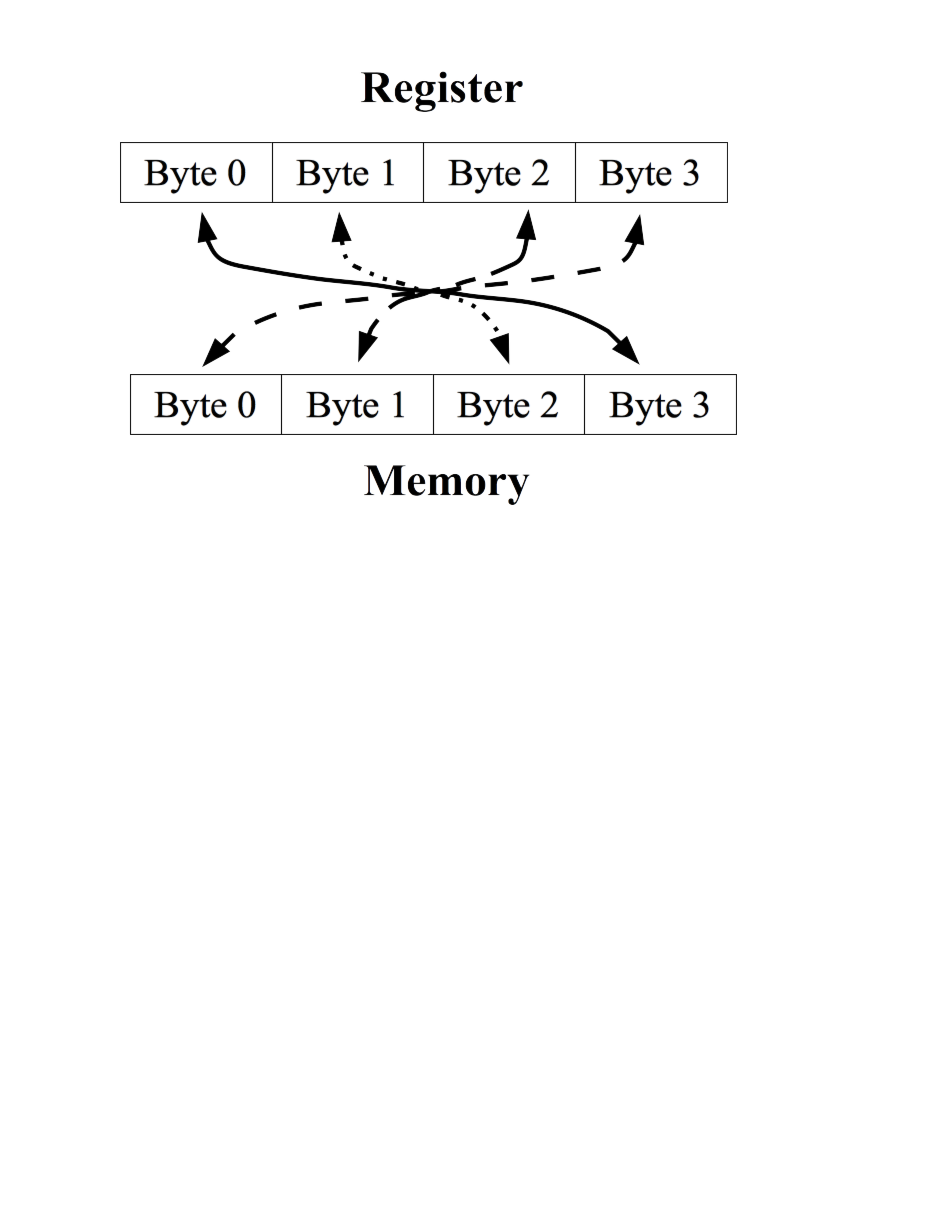
\includegraphics[width=\textwidth]{littleendian.png}
\end{figure}

Other processors are 
\emph{big-endian\index{big-endian}} processors, which means that they store 
the "big end", or most significant byte, of their words first, the way we would naturally read a number.

\begin{figure}
\caption{Register-to-memory transfers on big-endian systems}
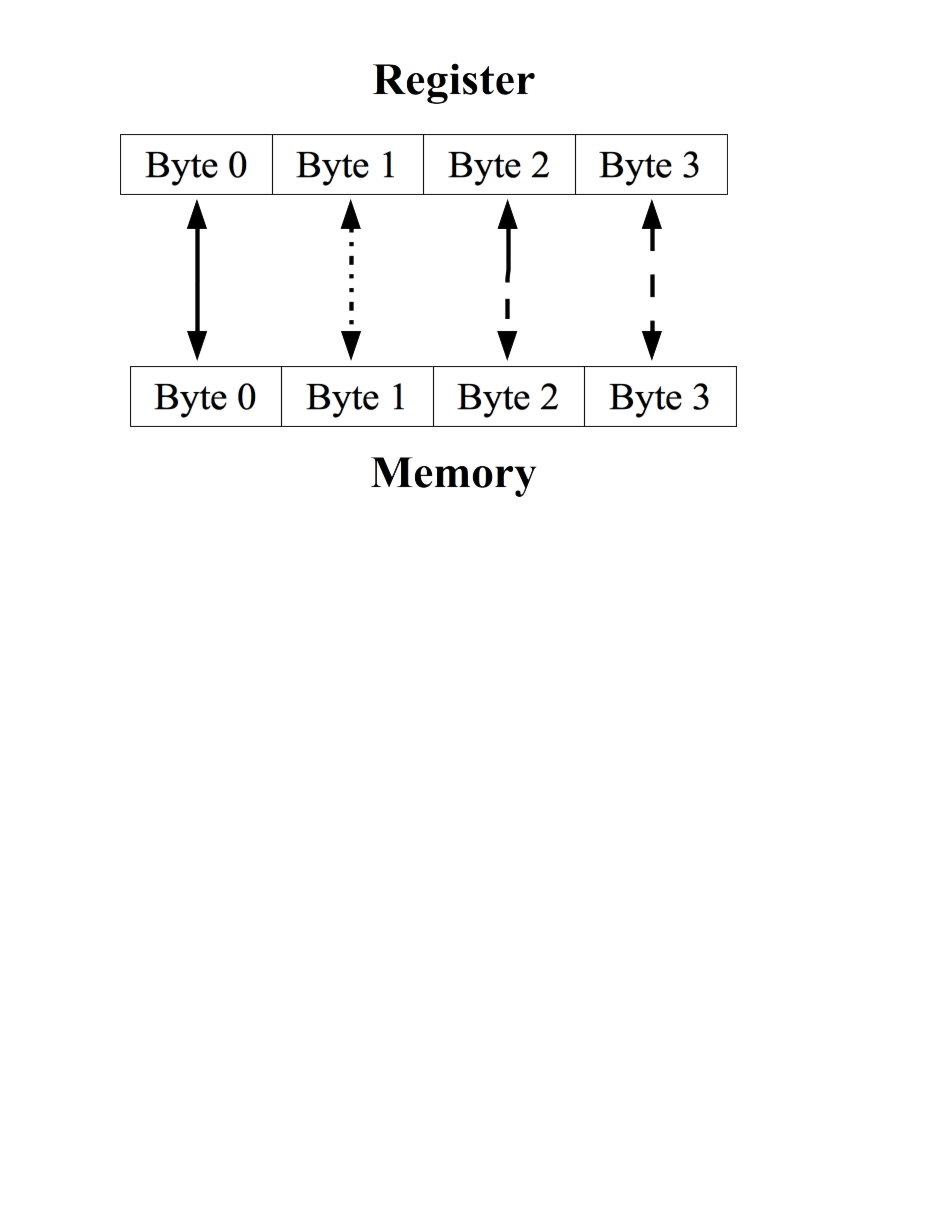
\includegraphics[width=\textwidth]{bigendian.png}
\end{figure}

This difference is not normally a problem (although it has sparked many
technical controversies throughout the years). 
Because the bytes are reversed again (or not, if it is a big-endian processor)
when being read back into a register\index{register}, the programmer usually never 
notices what order the bytes are in.  The byte-switching magic happens
automatically behind the scenes during register-to-memory transfers.  
However, the byte order can cause problems in several instances:

\begin{itemize}\item If you try to read in several bytes at a time using \icode{movl} but deal with them on a byte-by-byte basis using the least significant byte (i.e. - by using {\alReg} and/or shifting of the register), this will be in a different order than they appear in memory. 
\item If you read or write files written for different architectures, you may have to account for whatever order they write their bytes in. 
\item If you read or write to network sockets, you may have to account for a different byte order in the protocol. 
\end{itemize}

As long as you are aware of the issue, it usually isn't a big deal.  For more
in-depth look at byte order issues, you should read DAV's Endian FAQ at http://www.rdrop.com/~cary/html/endian\_faq.html, especially the article "On Holy Wars and a Plea for Peace" by Daniel Cohen.

\section{Converting Numbers for Display}

So far, we have been unable to display any number stored to the 
user, except by the extremely limitted means of passing it through
exit codes.  In this section, we will discuss converting positive numbers
into strings for display.

The function will be called \icode{integer2string}, and
it will take two parameters - an integer to convert and a string buffer 
filled with null characters (zeroes).  The buffer will be assumed to
be big enough to store the entire number as a string.(at least 11 characters
long, to include a trailing null character).

Remember that the way that we see numbers is in base 10.  Therefore, to access
the individual decimal digits of a number, we need to be dividing by 10
and displaying the remainder for each digit.  Therefore, the process will
look like this:

\begin{itemize}\item Divide the number by ten 
\item The remainder is the current digit.  Convert it to a character and store it. 
\item We are finished if the quotient is zero. 
\item Otherwise, take the quotient and the next location in the buffer and repeat the process. 
\end{itemize}

The only problem is that since this process deals with the one's place first,
it will leave the number backwards.  Therefore, we will have to finish by 
reversing the characters.  We will do this by storing the characters on
the stack as we compute them.  This way, as we pop them back off to fill
in the buffer, it will be in the reverse order that we pushed them on.

The code for the function should be put in a file called 
\icodefilename{integer-to-string.s} and should be entered as follows:

\begin{simpletyping}
\lstinputlisting{integer-to-string}
\end{simpletyping}

To show this used in a full program, use the following code, along
with the \icode{count\_chars} and \icode{write\_newline}
functions written about in previous chapters.  The code should be
in a file called \icodefilename{conversion-program.s}.

\begin{simpletyping}
\lstinputlisting{conversion-program}
\end{simpletyping}

To build the program, issue the following commands:

\begin{simpletyping}
\begin{lstlisting}
as integer-to-string.s -o integer-to-number.o
as count-chars.s -o count-chars.o
as write-newline.s -o write-newline.o
as conversion-program.s -o conversion-program.o
ld integer-to-number.o count-chars.o write-newline.o conversion-program.o -o conversion-program
\end{lstlisting}
\end{simpletyping}

To run just type \icode{./conversion-program} and the output
should say \icode{824}.

\section{Review}

\section{Know the Concepts}

\begin{itemize}\item Convert the decimal number 5,294 to binary. 
\item What number does 0x0234aeff represent?  Specify in binary, octal, and decimal. 
\item Add the binary numbers 10111001 and 101011. 
\item Multiply the binary numbers 1100 1010110. 
\item Convert the results of the previous two problems into decimal. 
\item Describe how AND, OR, NOT, and XOR work. 
\item What is masking for? 
\item What number would you use for the flags of the \icode{open} system call if you wanted to open the file for writing, and create the file if it doesn't exist? 
\item How would you represent -55 in a thirty-two bit register? 
\item Sign-extend the previous quantity into a 64-bit register. 
\item Describe the difference between little-endian and big-endian storage of words in memory. 
\end{itemize}

\section{Use the Concepts}

\begin{itemize}\item Go back to previous programs that returned numeric results through the exit status code, and rewrite them to print out the results instead using our integer to string conversion function. 
\item Modify the \icode{integer2string} code to return results in octal rather than decimal. 
\item Modify the \icode{integer2string} code so that the conversion base is a parameter rather than hardcoded. 
\item Write a function called \icode{is\_negative} that takes a single integer as a parameter and returns 1 if the parameter is negative, and 0 if the parameter is positive. 
\end{itemize}

\section{Going Further}

\begin{itemize}\item Modify the \icode{integer2string} code so that the conversion base can be greater than 10 (this requires you to use letters for numbers past 9). 
\item Create a function that does the reverse of \icode{integer2string} called \icode{number2integer} which takes a character string and converts it to a register-sized integer.  Test it by running that integer back through the \icode{integer2string} function and displaying the results. 
\item Write a program that stores likes and dislikes into a single machine word, and then compares two sets of likes and dislikes for commonalities. 
\item Write a program that reads a string of characters from STDIN and converts them to a number. 
\end{itemize}


\chapter{High-Level Languages}
\label{highlevellanguages}

% 
% 
% Copyright 2002 Jonathan Bartlett
% 
% Permission is granted to copy, distribute and/or modify this
% document under the terms of the GNU Free Documentation License,
% Version 1.1 or any later version published by the Free Software
% Foundation; with no Invariant Sections, with no Front-Cover Texts,
% and with no Back-Cover Texts.  A copy of the license is included in fdl.xml
% 

In this chapter we will begin to look at our first "real-world"
programming language.  Assembly language is the language used
at the machine's level, but most people find
coding in assembly language too cumbersome for everyday use.
Many computer languages have been invented to make the programming
task easier.  Knowing a wide variety of languages is useful for
many reasons, including

\begin{itemize}\item Different languages are based on different concepts, which will help you to learn different and better programming methods and ideas. 
\item Different languages are good for different types of projects. 
\item Different companies have different standard languages, so knowing more languages makes your skills more marketable. 
\item The more languages you know, the easier it is to pick up new ones. 
\end{itemize}

As a programmer, you will often have to pick up new languages.  Professional
programmers can usually pick up a new language with about a weeks
worth of study and practice.  Languages are simply tools, and learning
to use a new tool should not be something a programmer flinches at.  In fact,
if you do computer consulting you will often have to learn new languages
on the spot in order to keep yourself employed. It will often be your
customer, not you, who decides what language is used.  This
chapter will introduce you to a few of the languages available to you.  
I encourage you to explore as many languages as you are interested in.
I personally try to learn a new language every few months.

\section{Compiled and Interpreted Languages}

Many languages are \emph{compiled} languages.  
When you write assembly language\index{assembly language}, each instruction you write is 
translated into
exactly one machine instruction for processing.  With compilers\index{compilers},
a statement can translate into one or hundreds of machine 
instructions.  In fact, depending on how advanced your compiler
is, it might even restructure parts of your code to make it faster.
In assembly language what you write is what you get.

There are also languages that are \emph{interpreted}
languages.  These languages require that the user run a program
called an \emph{interpreter\index{interpreter}} that in turn runs the
given program.  These are usually slower than compiled programs,
since the interpreter has to read and interpret the code as it goes 
along.  However, in well-made interpreters, this time can be
fairly negligible.  There is also a class of hybrid languages
which partially compile a program before execution into byte-codes.
This is done because the interpreter
can read the byte-codes much faster than it can read the regular language.

There are many reasons to choose one or the other.  Compiled programs
are nice, because you don't have to already have an interpreter installed
in the user's machine.  You have to have a compiler for the language,
but the users of your program don't.  In an interpreted language, you
have to be sure that the user has an interpreter installed for your program,
and that the computer knows which interpreter to run your program with.  However,
interpeted languages tend to be more flexible, while compiled languages
are more rigid.

Language choice is usually driven by available tools and support for 
programming methods rather than by whether a language is compiled
or interpretted.  In fact many languages have options for either one.  

High-level languages, whether compiled or interpreted, are oriented around
you, the programmer, instead of around the machine.  This opens them up
to a wide variety of features, which can include the following:

\begin{itemize}\item Being able to group multiple operations into a single expression 
\item Being able to use "big values" - values that are much more conceptual than the 4-byte words that computers normally deal with (for example, being able to view text strings as a single value rather than as a string of bytes). 
\item Having access to better flow control\index{flow control} constructs than just jumps. 
\item Having a compiler to check types of value assignments and other assertions. 
\item Having memory handled automatically. 
\item Being able to work in a language that resembles the problem domain rather than the computer hardware. 
\end{itemize}

So why does one choose one language over another?
For example, many choose Perl because it has a vast library of functions
for handling just about every protocol or type of data on the planet.
Python, however, has a cleaner syntax and often lends itself to more 
straightforward solutions.  Its cross-platform GUI tools are also excellent.  
PHP makes writing web applications simple.  Common LISP has more power and
features than any other environment for those willing to learn it.  Scheme is
the model of simplicity and power combined together.  C is easy to interface
with other languages.

Each language is different, and the more 
languages you know the better programmer you will be.  Knowing the
concepts of different languages will help you in all programming, because
you can match the programming language to the problem better, and you
have a larger set of tools to work with.  Even if certain features aren't
directly supported in the language you are using, often they can be simulated.
However, if you don't have a broad experience with languages, you won't
know of all the possibilities you have to choose from.

\section{Your First C Program}

\index{C Programming Language}
Here is your first C program,
which prints "Hello world" to the screen and exits.  Type it in, and
give it the name Hello-World.c

\begin{simpletyping}
\lstinputlisting{Hello-World.c}
\end{simpletyping}

As you can see, it's a pretty simple program.  To compile it,
run the command

\begin{simpletyping}
\begin{lstlisting}
gcc -o HelloWorld Hello-World.c
\end{lstlisting}
\end{simpletyping}

To run the program, do

\begin{simpletyping}
\begin{lstlisting}
./HelloWorld
\end{lstlisting}
\end{simpletyping}

Let's look at how this program was put together.

Comments in C are started with \icode{/*} and ended with
\icode{*/}.  Comments can span multiple lines, but 
many people prefer to start and end comments on the same line
so they don't get confused.

\icode{\#include <stdio.h>}
\index{stdio.h}
 is the first part of
the program.  This is a \emph{preprocessor directive}.
C compiling is split into two stages - the preprocessor\index{preprocessor} and the
main compiler.  This directive tells the preprocessor to look
for the file \icodefilename{stdio.h} and paste it into
your program.  The preprocessor is responsible for putting together the
text of the program.  This includes sticking different files together, running
macros on your program text, etc.  After the text is put together, the 
preprocessor is done and the main compiler goes to work.

Now, everything in \icodefilename{stdio.h} is
now in your program just as if you typed it there yourself.  The angle brackets
around the filename tell the compiler to look in its standard
paths for the file (\icodefilename{/usr/include\index{/usr/include}} and 
\icodefilename{/usr/local/include\index{/usr/local/include}}, usually).  If it was
in quotes, like \icode{\#include "stdio.h"} it would
look in the current directory for the file.  Anyway, 
\icodefilename{stdio.h} contains the declarations for 
the standard input and output functions and variables.   These
declarations tell the
compiler what functions are available for input and output.  The next few
lines are simply comments about the program.

Then there is the line \icode{int main(int argc, char **argv)}.
This is the start of a function.  C Functions are declared with their 
name, arguments and return type.  This declaration says that the function's
name is \icode{main}, it returns an \icode{int} 
(integer - 4 bytes long on the x86 platform), and has two arguments - 
an \icode{int} called
\icode{argc} and a \icode{char **} called 
\icode{argv}.  You don't have to worry about where the arguments
are positioned on the stack - the C compiler takes care of that for you.
You also don't have to worry about loading values into and out of registers
because the compiler takes care of that, too.

The \icode{main} function is a special function in the
C language - it is the
start of all C programs (much like \icode{\_start} in our
assembly-language programs).  It always takes two parameters.  The first 
parameter is the number of arguments given to this command, and the
second parameter is a list of the arguments that were given.

The next line is a function call.  In assembly language, you had to 
push the arguments of a function onto the stack, and then call the function.
C takes care of this complexity for you.  You simply have to call the
function with the parameters in parenthesis.  In this case, we call
the function \icode{puts}, with a single parameter.  This
parameter is the character string we want to print.  We just have to
type in the string in quotations, and the compiler takes care of defining
storage and moving the pointers to that storage onto the stack before
calling the function.  As you can see, it's a lot less work.

Finally our function returns the number \icode{0}.  In assembly
language, we stored our return value in {\eaxReg}, but in C we just use
the \icode{return} command and it takes care of that for us.
The return value of the \icode{main} function is what is
used as the exit code for the program.

As you can see, using high-level languages\index{high-level languages} makes life much easier.
It also allows our programs to run on multiple platforms more easily.
In assembly language, your program is tied to both the operating system
and the hardware platform, while in compiled and interpreted languages
the same code can usually run on multiple operating systems and hardware
platforms.  For example, this program can be built and executed on x86
hardware running Linux\textregistered, Windows\textregistered, UNIX\textregistered, or most other operating systems.
In addition, it can also run on Macintosh hardware running a number of
operating systems.

Additional information on the C programming language can be found in
\autoref{ctranslationap}.

\section{Perl}

Perl is an interpreted language, existing mostly on Linux and UNIX-based
platforms.  It actually runs on almost all platforms, but you find it most
often on Linux and UNIX-based ones.  Anyway, here is the Perl version
of the program, which should be typed into a file named 
\icodefilename{Hello-World.pl}:

\begin{simpletyping}
\lstinputlisting{Hello-World.pl}
\end{simpletyping}

Since Perl is interpreted, you don't need to compile or link it.  Just
run in with the following command:

\begin{simpletyping}
\begin{lstlisting}
perl Hello-World.pl
\end{lstlisting}
\end{simpletyping}

As you can see, the Perl\index{Perl} version is even shorter than the C version.
With Perl you don't have to declare any functions or program entry points.
You can just start typing commands and the interpreter will run them
as it comes to them.  In fact this program only has two lines of code,
one of which is optional.

The first, optional line is used for UNIX machines to tell which interpreter
to use to run the program.  The \icode{\#!} tells the computer
that this is an interpreted program, and the 
\icodefilename{/usr/bin/perl} tells the computer to use the program
\icodefilename{/usr/bin/perl} to interpret the program.  However, since
we ran the program by typing in \icode{perl Hello-World.pl}, we
had already specified that we were using the perl interpreter.

The next line calls a Perl builtin function, print.  This has one parameter,
the string to print.  The program doesn't have an explicit return
statement - it knows to return simply because it runs off the end of the file.
It also knows to return 0 because there were no errors while it ran.  You can
see that interpreted languages are often focused on letting you get working 
code as quickly as possible, without having to do a lot of extra legwork.

One thing about Perl that isn't so evident from this example is that Perl
treats strings as a single value.  In assembly language, we had to program
according to the computer's memory architecture, which meant that strings
had to be treated as a sequence of multiple values, with a pointer to the
first letter.  Perl pretends that strings can be stored directly as values,
and thus hides the complication of manipulating them for you.  In fact,
one of Perl's main strengths is its ability and speed at manipulating
text.  

\section{Python}

The Python\index{Python} version of the program looks almost exactly like the Perl one.
However, Python is really a very different language than Perl, even if
it doesn't seem so from this trivial example.  Type the program into
a file named \icodefilename{Hello-World.py}.  The program follows:

\begin{simpletyping}
\lstinputlisting{Hello-World.py}
\end{simpletyping}

You should be able to tell what the different lines of the program do.

\section{Review}

\section{Know the Concepts}

\begin{itemize}\item What is the difference between an intepretted language and a compiled language? 
\item What reasons might cause you to need to learn a new programming language? 
\end{itemize}

\section{Use the Concepts}

\begin{itemize}\item Learn the basic syntax of a new programming language.  Re-code one of the programs in this book in that language. 
\item In the program you wrote in the question above, what specific things were automated in the programming language you chose? 
\item Modify your program so that it runs 10,000 times in a row, both in assembly language and in your new language.  Then run the \icode{time} command to see which is faster.  Which does come out ahead?  Why do you think that is? 
\item How does the programming language's input/output methods differ from that of the Linux system calls? 
\end{itemize}

\section{Going Further}

\begin{itemize}\item Having seen languages which have such brevity as Perl, why do you think this book started you with a language as verbose as assembly language? 
\item How do you think high level languages have affected the process of programming? 
\item Why do you think so many languages exist? 
\item Learn two new high level languages.  How do they differ from each other?  How are they similar?  What approach to problem-solving does each take? 
\end{itemize}

% 
% 
% Advanced Linking Techniques
% 
% LD\_PRELOAD
% 
% loading a library on the fly
% 
% static libraries
% 
% sonames
% 
% ELF sections and special sections (.ini .fini or whatever)
% 
% Process for loading and linking ELF files
% 
% Other object file types (COFF a.out)
% 
% The file format used to store programs in Linux is called ELF, which
% stands for "Executable and Linking Format".  ELF is very flexible,
% but it is also fairly complex.  Let's take a look at how we've
% been using ELF so far.
% 

% 
% <sect2>
% \textbf{ELF Sections}
% 

% The \icode{.section} directives we've been using
% are commands that tell the linker, \icode{ld}, to
% group things together.  There are many predefined sections.
% The ones we mainly use are \icode{.data} and 
% \icode{.text}.  In your assembly code, you can mix
% \icode{.data} and \icode{.text} sections,
% and the linker will put everything in a section together.  Let's
% take a look at one of our files.  Let's look at the 
% \icode{toupper} file we created earlier.  If you
% run the command \icode{objdump -h toupper}, you will
% get a listing that looks like this:
% 

% 
% 


\chapter{Optimization}
\label{optimizationch}

% 
% 
% Copyright 2002 Jonathan Bartlett
% 
% Permission is granted to copy, distribute and/or modify this
% document under the terms of the GNU Free Documentation License,
% Version 1.1 or any later version published by the Free Software
% Foundation; with no Invariant Sections, with no Front-Cover Texts,
% and with no Back-Cover Texts.  A copy of the license is included in fdl.xml
% 

Optimization\index{optimization} is the process of making your application run more
effectively.  You can optimize for many things - speed, memory
space usage, disk space usage, etc. This chapter, however, 
focuses on speed optimization.

\section{When to Optimize}

It is better to not optimize at all than to optimize too soon.  When you
optimize, your code generally becomes less clear, because it becomes
more complex.  Readers of your code will have more trouble discovering
why you did what you did which will increase the cost of maintenance 
of your project.  Even when you know how and why your program runs the way
it does, optimized code is harder to debug and extend.  It slows the
development process down considerably, both because of the time it
takes to optimize the code, and the time it takes to modify your 
optimized code.

Compounding this problem is that you don't even know beforehand where
the speed issues in your program will be.  Even experienced programmers
have trouble predicting which parts of the program will be the bottlenecks
which need optimization,
so you will probably end up wasting your time optimizing the wrong parts.
\autoref{wheretooptimize} will discuss how to find the parts of
your program that need optimization.

While you develop your program, you need to have the following priorities:

\begin{itemize}\item Everything is documented 
\item Everything works as documented 
\item The code is written in an modular, easily modifiable form 
\end{itemize}

Documentation\index{documentation} is essential, especially when working in groups.  The proper
functioning of the program is essential.  
You'll notice application speed was not anywhere on that list.  Optimization is
not necessary during early development for the following reasons:

\begin{itemize}\item Minor speed problems can be usually solved through hardware, which is often much cheaper than a programmer's time. 
\item Your application will change dramatically as you revise it, therefore wasting most of your efforts to optimize it.\footnote{Many
new projects often have a first code base which is completely rewritten
as developers learn more about the problem they are trying to solve.  Any
optimization done on the first codebase is completely wasted.} 
\item Speed problems are usually localized in a few places in your code - finding these is difficult before you have most of the program finished. 
\end{itemize}

Therefore, the time to optimize is toward the end of development, when you
have determined that your correct code actually has performance problems. 

In a web-based e-commerce project I was involved in, I focused entirely on 
correctness.  This was much to the dismay of my colleagues, who were worried
about the fact that each page took twelve seconds to process before it ever
started loading (most web pages process in under a second).  However, I
was determined to make it the right way first, and put optimization as a 
last priority.  When the code was finally correct after 3 months of work,
it took only three days to find and eliminate the bottlenecks, bringing
the average processing time under a quarter of a second.  By focusing on the
correct order, I was able to finish a project that was both correct and
efficient.

\section{Where to Optimize}
\label{wheretooptimize}

Once you have determined that you have a performance issue you need
to determine where in the code the problems occur.  You can do this
by running a 
\emph{profiler}\index{profiler}.
A profiler is a program that will let you run your program, and it
will tell you how much time is spent in each function, and how many
times they are run.  \icode{gprof\index{gprof}} is the standard GNU/Linux
profiling tool, but a discussion of using profilers is outside 
the scope of this text.  After running a profiler, you can determine which
functions are called the most or have the most time spent in them.  These
are the ones you should focus your optimization efforts on.

If a program only spends 1\% of its time in a given function, then no matter 
how much you speed it up you will only achieve a 
\emph{maximum} of a 1\% overall speed improvement.
However, if a program spends 20\% of its time in a given function, then even
minor improvements to that functions speed will be noticeable.  Therefore,
profiling gives you the information you need to make good choices about
where to spend your programming time.

In order to optimize functions, you need to understand in what ways they
are being called and used.  The more you know about how and when a function
is called, the better position you will be in to optimize it appropriately.

There are two main categories of optimization - local optimizations\index{local optimizations} and
global optimizations\index{global optimizations}.  Local optimizations consist of optimizations that are
either hardware specific - such as the fastest way to perform a given
computation - or program-specific - such as making a specific piece of
code perform the best for the most often-occuring case.  Global optimization
consist of optimizations which are structural.  For example, if you were
trying to find the best way for three people in different cities to meet in
St. Louis, a local optimization would be finding a better road to get there,
while a global optimization would be to decide to teleconference instead of
meeting in person.  Global optimization often involves restructuring code
to avoid performance problems, rather than trying to find the best way 
through them.

\section{Local Optimizations}

The following are some well-known methods of optimizing pieces of code.  When
using high level languages, some of these may be done automatically by your
compiler's optimizer.

\begin{description}
\item[Precomputing Calculations] Sometimes a function has a limitted number of possible inputs and outputs.  In
fact, it may be so few that you can actually precompute all of the possible
answers beforehand, and simply look up the answer when the function is called.
This takes up some space since you have to store all of the answers, but for
small sets of data this works out really well, especially if the computation
normally takes a long time.
\item[Remembering Calculation Results] This is similar to the previous method, but instead of computing results
beforehand, the result of each calculation requested is stored.  This way
when the function starts, if the result has been computed before it will
simply return the previous answer, otherwise it will do the full computation
and store the result for later lookup.  This has the advantage of requiring
less storage space because you aren't precomputing all results.  This
is sometimes termed \emph{caching\index{caching}} or \emph{memoizing\index{memoizing}}.
\item[Locality of Reference] \emph{Locality of reference\index{locality of reference}} is a term for where in memory the 
data items you are accessing are.  With virtual memory, you may access pages
of memory which are stored on disk.  In such a case, the operating system has
to load that memory page from disk, and unload others to disk.  Let's say, 
for instance, that the operating system will allow you to have 20k of memory
in physical memory and forces the rest of it to be on disk, and your 
application uses 60k of memory.  Let's say your program has to do 5 operations 
on each piece of data.  If it does one operation on every piece of data, and 
then goes through and does the next operation on each piece of data, eventually
every page of data will be loaded and unloaded from the disk 5 times.  Instead,
if you did all 5 operations on a given data item, you only have to load each
page from disk once.  When you bundle as many operations on data that is
physically close to each other in memory, then you are taking advantage of 
locality of reference.  In addition, processors usually store some data on-chip
in a cache\index{cache}.  If you keep all of your operations within a small area of 
physical memory\index{physical memory}, your program may bypass even main memory and only use the chip's ultra-fast cache
memory.  This is all done for you - all you have to do is to try to operate on
small sections of memory at a time, rather than bouncing all over the place.
\item[Register Usage] Registers\index{registers} are the fastest memory locations on the computer.  When you access
memory, the processor has to wait while it is loaded from the 
memory bus.  However, registers are located on the processor itself, 
so access is extremely fast.  Therefore making wise usage of registers 
is extremely important.  If you have few enough data items you are working 
with, try to store them all in registers.  In high level languages,
you do not always have this option - the compiler decides what goes in 
registers and what doesn't.
\item[Inline Functions] Functions are great from the point of view of program management - they 
make it easy to break up your program into independent, understandable, 
and reuseable parts.  However, function calls do involve the overhead of 
pushing arguments onto the stack and doing the jumps (remember locality  of 
reference - your code may be swapped out on disk instead of in memory).  
For high level languages, it's often impossible for compilers to do 
optimizations across function-call 
boundaries.  However, some languages support inline functions\index{inline functions} or function macros\index{macros}.  These 
functions look, smell, taste, and act like real functions, except the 
compiler has the option to simply plug the code in exactly where it was 
called.  This makes the program faster, but it also increases the size 
of the code.  There are also many functions, like recursive functions, 
which cannot be inlined because they call themselves either directly or 
indirectly.
\item[Optimized Instructions] Often times there are multiple assembly language instructions which 
accomplish the same purpose.   A skilled assembly language programmer 
knows which instructions are the fastest.  However, this can change 
from processor to processor.  For more information on this topic, you need to 
see the user's manual that is provided for the specific chip you are using.  
As an example, let's look at the process of loading the number 0 into a 
register.  On most processors, doing a \icode{movl \$0, {\eaxBare}} is 
not the quickest way.  The quickest way is to exclusive-or the register with 
itself, \icode{xorl {\eaxBare}, {\eaxBare}}.  This is because it only has
to access the register, and doesn't have to transfer any data.  
For users of high-level languages, the compiler handles this kind of 
optimizations for you.  For assembly-language programmers, you
need to know your processor well.
\item[Addressing Modes] Different addressing modes\index{addressing modes} work at different speeds.  The fastest are 
the immediate\index{immediate mode addressing} and register addressing modes.  Direct\index{direct addressing mode} is the next fastest, 
indirect is next, and base pointer\index{base pointer addressing mode} and indexed indirect\index{indexed indirect addressing mode} are the slowest.  
Try to use the faster addressing modes, when possible.  One interesting
consequence of this is that when you have a structured piece of memory 
that you are accessing using base pointer addressing, the first element can 
be accessed the quickest.  Since its offset is 0, you can access it using 
indirect addressing instead of base pointer addressing, which makes it 
faster.
\item[Data Alignment] Some processors can access data on word-aligned memory\index{aligned memory} boundaries 
(i.e. - addresses divisible by the word size) faster than non-aligned data.  
So, when setting up structures in memory, it is best to keep it word-aligned.  
Some non-x86 processors, in fact, cannot access non-aligned data in some modes.
\end{description}

These are just a smattering of examples of the kinds of local optimizations 
possible.  However, remember that the maintainability and readability of 
code is much more important except under extreme circumstances.

\section{Global Optimization}

Global optimization\index{global optimizations} has two goals.  The first one is to put your code
in a form where it is easy to do local optimiztions.  For example, 
if you have a large procedure that 
performs several slow, complex calculations, you might see if you can break
parts of that procedure into their own functions where the
values can be precomputed or memoized. 

Stateless functions\index{stateless functions} (functions that only operate on the parameters that
were passed to them - i.e. no globals or system calls) are the easiest 
type of functions to optimize in a computer.  The more stateless parts of 
your program you have, the more opportunities you have to optimize.  In the
e-commerce situation I wrote about above, the computer had to find all of 
the associated parts for specific inventory items.  This required about 12
database calls, and in the worst case took about 20 seconds.  However, the goal
of this program was to be interactive, and a long wait
would destroy that goal.  However, I knew that these inventory
configurations do not change.  Therefore, I converted the 
database calls into their own functions, which were stateless.
I was then able to memoize the functions.  At the beginning of
each day, the function results were cleared in case anyone had
changed them, and several inventory items were automatically
preloaded.  From then on during the day, the first time someone
accessed an inventory item, it would take the 20 seconds it
did beforehand, but afterwards it would take less than a second,
because the database results had been memoized.

Global optimization usually often involves achieving the following 
properties in your functions:

\begin{description}
\item[Parallelization] Parallelization\index{parallelization} means that your algorithm
can effectively be split among multiple processes.  For example, 
pregnancy is not very parallelizable because no matter how many women
you have, it still takes nine months.  However, building a car is
parallelizable because you can have one worker working on the engine
while another one is working on the interior.  Usually, applications
have a limit to how parallelizable they are.  The more parallelizable
your application is, the better it can take advantage of multiprocessor
and clustered computer configurations.
\item[Statelessness] As we've discussed, stateless\index{stateless functions} functions and programs are those that rely 
entirely on the data explicitly passed to them for functioning.  
Most processes are not entirely stateless, but they can be within
limits.  In my e-commerce example, the function wasn't entirely stateless,
but it was within the confines of a single day.  Therefore, I optimized it
as if it were a stateless function, but made allowances for changes at night.
Two great benefits resulting from statelessness is that most stateless 
functions are parallelizable and often benefit from memoization.
\end{description}

Global optimization takes quite a bit of practice to know what works and
what doesn't.  Deciding how to tackle optimization problems in code involves
looking at all the issues, and knowing that fixing some issues may cause others.

\section{Review}

\section{Know the Concepts}

%  FIXME - Dominique suggestion - have an appendix with multiple versions of optimized code 

\begin{itemize}\item At what level of importance is optimization compared to the other priorities in programming? 
\item What is the difference between local and global optimizations? 
\item Name some types of local optimizations. 
\item How do you determine what parts of your program need optimization? 
\item At what level of importance is optimization compared to the other priorities in programming?  Why do you think I repeated that question? 
\end{itemize}

\section{Use the Concepts}

\begin{itemize}\item Go back through each program in this book and try to make optimizations according to the procedures outlined in this chapter 
\item Pick a program from the previous exercise and try to calculate the performance impact on your code under specific inputs.\footnote{Since these programs are usually short enough not to have noticeable performance problems, looping through the program thousands of times will exaggerate the time it takes to run enough to make calculations.} 
\end{itemize}

\section{Going Further}

\begin{itemize}\item Find an open-source program that you find particularly fast.  Contact one of the developers and ask about what kinds of optimizations they performed to improve the speed. 
\item Find an open-source program that you find particularly slow, and try to imagine the reasons for the slowness.  Then, download the code and try to profile it using \icode{gprof} or similar tool.  Find where the code is spending the majority of the time and try to optimize it.  Was the reason for the slowness different than you imagined? 
\item Has the compiler eliminated the need for local optimizations?  Why or why not? 
\item What kind of problems might a compiler run in to if it tried to optimize code across function call boundaries? 
\end{itemize}


\chapter{Moving On from Here}
\label{wherenextch}

% 
% 
% Copyright 2002 Jonathan Bartlett
% 
% Permission is granted to copy, distribute and/or modify this
% document under the terms of the GNU Free Documentation License,
% Version 1.1 or any later version published by the Free Software
% Foundation; with no Invariant Sections, with no Front-Cover Texts,
% and with no Back-Cover Texts.  A copy of the license is included in fdl.xml
% 

Congratulations on getting this far.  You should now have a basis for 
understanding the issues involved in many areas of programming.  Even
if you never use assembly language again, you have gained a valuable
perspective and mental framework for understanding the rest of computer
science. 

There are essentially three methods to learn to program:

\begin{itemize}\item From the Bottom Up - This is how this book teaches.  It starts with low-level programming, and works toward more generalized teaching. 
\item From the Top Down - This is the opposite direction.  This focuses on what you want to do with the computer, and teaches you how to break it down more and more until you get to the low levels. 
\item From the Middle - This is characterized by books which teach a specific programming language or API.  These are not as concerned with concepts as they are with specifics. 
\end{itemize}

Different people like different approaches, but a good programmer takes all of 
them into account.  The bottom-up approaches help you understand the machine 
aspects, the top-down approaches help you understand the problem-area aspects,
and the middle approaches help you with practical questions and answers.  To
leave any of these aspects out would be a mistake.

Computer Programming is a vast subject.  As a programmer, you will need
to be prepared to be constantly learning and pushing your limits.  These
books will help you do that.  They not only teach their subjects, but also
teach various ways and methods of \emph{thinking}.  As
Alan Perlis said, "A language that doesn't affect the way you think about
programming is not worth knowing" 
(http://www.cs.yale.edu/homes/perlis-alan/quotes.html).  If you are 
constantly looking for new and better ways of doing and thinking, you
will make a successful programmer.  If you do not seek to enhance yourself,
"A little sleep, a little slumber, a little folding of the hands to rest - 
and poverty will come on you like a bandit and scarcity like an armed man."
(Proverbs 24:33-34 NIV).  Perhaps not quite that severe, but still, it is best
to always be learning.

These books were selected because of their content and the amount of respect
they have in the computer science world.  Each of them brings something
unique.  There are many books here.  The best way to start would be to
look through online reviews of several of the books, and find a starting
point that interests you.

\section{From the Bottom Up}

This list is in the best reading order I could find.  It's not necessarily
easiest to hardest, but based on subject matter.  

\begin{itemize}\item \documentname{Programming from the Ground Up} by Jonathan Bartlett 
\item \documentname{Introduction to Algorithms} by Thomas H. Cormen, Charles E. Leiserson, and Ronald L. Rivest 
\item \documentname{The Art of Computer Programming} by Donald Knuth (3 volume set - volume 1 is the most important) 
\item \documentname{Programming Languages} by Samuel N. Kamin 
\item \documentname{Modern Operating Systems} by Andrew Tanenbaum 
\item \documentname{Linkers and Loaders} by John Levine 
\item \documentname{Computer Organization and Design: The Hardware/Software Interface} by David Patterson and John Hennessy 
\end{itemize}

\section{From the Top Down}

These books are arranged from the simplest to the hardest.  However, they
can be read in any order you feel comfortable with.

\begin{itemize}\item \documentname{How to Design Programs} by Matthias Felleisen, Robert Bruce Findler, Matthew Flatt, and Shiram Krishnamurthi, available online at http://www.htdp.org/ 
\item \documentname{Simply Scheme: An Introduction to Computer Science} by Brian Harvey and Matthew Wright 
\item \documentname{How to Think Like a Computer Scientist: Learning with Python} by Allen Downey, Jeff Elkner, and Chris Meyers, available online at http://www.greenteapress.com/thinkpython/ 
\item \documentname{Structure and Interpretation of Computer Programs} by Harold Abelson and Gerald Jay Sussman with Julie Sussman, available online at http://mitpress.mit.edu/sicp/ 
\item \documentname{Design Patterns} by Erich Gamma, Richard Helm, Ralph Johnson, and John Vlissides 
\item \documentname{What not How: The Rules Approach to Application Development} by Chris Date 
\item \documentname{The Algorithm Design Manual} by Steve Skiena 
\item \documentname{Programming Language Pragmatics} by Michael Scott 
\item \documentname{Essentials of Programming Languages} by Daniel P. Friedman, Mitchell Wand, and Christopher T. Haynes 
\end{itemize}

\section{From the Middle Out}

Each of these is the best book on its subject.  If you need to know these
languages, these will tell you all you need to know.

\begin{itemize}\item \documentname{Programming Perl} by Larry Wall, Tom Christiansen, and Jon Orwant 
\item \documentname{Common LISP: The Language} by Guy R. Steele 
\item \documentname{ANSI Common LISP} by Paul Graham 
\item \documentname{The C Programming Language} by Brian W. Kernighan and Dennis M. Ritchie 
\item \documentname{The Waite Group's C Primer Plus} by Stephen Prata 
\item \documentname{The C++ Programming Language} by Bjarne Stroustrup 
\item \documentname{Thinking in Java} by Bruce Eckel, available online at http://www.mindview.net/Books/TIJ/ 
\item \documentname{The Scheme Programming Language} by Kent Dybvig 
\item \documentname{Linux Assembly Language Programming} by Bob Neveln 
\end{itemize}

\section{Specialized Topics}

These books are the best books that cover their topic.  They are thorough and
authoritative.  To get a broad base of knowledge, you should read several
outside of the areas you normally program in.

\begin{itemize}\item Practical Programming - \documentname{Programming Pearls} and \documentname{More Programming Pearls} by Jon Louis Bentley 
\item Databases - \documentname{Understanding Relational Databases} by Fabian Pascal 
\item Project Management - \documentname{The Mythical Man-Month} by Fred P. Brooks 
\item UNIX Programming - \documentname{The Art of UNIX Programming} by Eric S. Raymond, available online at http://www.catb.org/~esr/writings/taoup/ 
\item UNIX Programming - \documentname{Advanced Programming in the UNIX Environment} by W. Richard Stevens 
\item Network Programming - \documentname{UNIX Network Programming} (2 volumes) by W. Richard Stevens 
\item Generic Programming - \documentname{Modern C++ Design} by Andrei Alexandrescu 
\item Compilers - \documentname{The Art of Compiler Design: Theory and Practice} by Thomas Pittman and James Peters 
\item Compilers - \documentname{Advanced Compiler Design and Implementation} by Steven Muchnick 
\item Development Process - \documentname{Refactoring: Improving the Design of Existing Code} by Martin Fowler, Kent Beck, John Brant, William Opdyke, and Don Roberts 
\item Typesetting - \documentname{Computers and Typesetting} (5 volumes) by Donald Knuth 
\item Cryptography - \documentname{Applied Cryptography} by Bruce Schneier 
\item Linux - \documentname{Professional Linux Programming} by Neil Matthew, Richard Stones, and 14 other people 
\item Linux Kernel - \documentname{Linux Device Drivers} by Alessandro Rubini and Jonathan Corbet 
\item Open Source Programming - \documentname{The Cathedral and the Bazaar: Musings on Linux and Open Source by an Accidental Revolutionary} by Eric S. Raymond 
\item Computer Architecture - \documentname{Computer Architecture: A Quantitative Approach} by David Patterson and John Hennessy 
\end{itemize}

\section{Further Resources on Assembly Language}

In assembly language, your best resources are on the web.

\begin{itemize}\item http://www.linuxassembly.org/ - a great resource for Linux assembly language programmers 
\item http://www.sandpile.org/ - a repository of reference material on x86, x86-64, and compatible processors 
\item http://www.x86.org/ - Dr. Dobb's Journal Microprocessor Resources 
\item http://www.drpaulcarter.com/pcasm/ - Dr. Paul Carter's PC Assembly Language Page 
\item http://webster.cs.ucr.edu/ - The Art of Assembly Home Page 
\item http://www.intel.com/design/pentium/manuals/ - Intel's manuals for their processors 
\item http://www.janw.easynet.be/ - Jan Wagemaker's Linux assembly language examples 
\item http://www.azillionmonkeys.com/qed/asm.html - Paul Hsieh's x86 Assembly Page 
\end{itemize}

% 
% 

% As you learn more, continue trying to build it upon the foundation you
% have already laid.  When you learn new languages and APIs, remember that
% they all eventually go down to the assembly language level.  It's nothing
% that you couldn't do yourself if you had the time.  Everything is within
% a reaching distance.
% 

% 
% 

% That said, you still have much to learn which is not covered by this book.  
% This chapter describes what you need to learn, and where to find that 
% information.  In fact, programming is only one part of what programmers
% do.  Programmers generally need to be knowledgeable in the following areas:
% 
% \begin{itemize}% \item Logical Data Organization 
% \item Physical Data Organization 
% \item Program Architecture 
% \item Project Management 
% \item System Administration and Networking 
% \item Security 
% \end{itemize}
% 

% 
% <sect1>
% \textbf{Logical Data Organization}
% 
% 

% Programs operate on data.  They are used to process data, produce new data,
% and be used for data entry.  Therefore, knowing about data organization
% is extremely important.  Logical data organization is mostly learning how
% to define the relationships between data.  Note that logical organization
% is simply how data are related to each other logically, not how it is actually
% stored within a computer.  Learning about relational
% databases is probably the best way to gain skill in this area.<footnote>
% 

Please note that learning SQL is not all there is to know about 
% databases and logical data organization.

</footnote>  Books that
% will help you in this area are:
% 
% \begin{itemize}% \item  
% \end{itemize}
% 
% 

% 
% 
% 
% <sect1>
% \textbf{Physical Data Organization}
% 
% 

% Physical data organization consists of methods of storing data on a computer
% for retrieval and update.  This field is mostly referred to as data structures.
% This book only really talks about two data structures - the array and
% the linked list.  However, there are many other data structures available
% to you as a programmer.  Having a background in assembly language will
% help you understand data structure design much better.
% 

% 
% 

% The following books are great ones for learning about data structures:
% 
% \begin{itemize}% \end{itemize}
% 

% 
% 
% 
% <sect1>
% \textbf{Program Architecture}
% 
% 

% Program architecture, or how to design and write programs effectively,
% is not taught in this book.  This book teaches the concepts of how 
% programming works, but not how to go about designing and writing a
% large-scale program.   The best books on this subject are:
% 
% \begin{itemize}% \end{itemize}
% 
% In addition to these books, one of the best ways to learn good program
% design techniques is to read well-architected programs.  The Free Software
% and Open Source communities contain a number of programs which can show
% you great programming practices on both large and small scales.
% 

% 
% 
% 
% <sect1>
% \textbf{Project Management}
% 
% 

% A lot of programming is project management - learning to gather requirements,
% calculate return on investment, estimate schedules, talk to people about
% requirements, status reports, etc.  Contrary to popular thought, successful
% programmers almost always have excellent communication skills, especially
% with nontechnical people.  Being able to communicate technical problems 
% and options to nontechnical people is an essential skill.  Being able to
% listen to nontechnical people and translating their needs into technical
% requirements is also an essential skill.  Programming without effective
% communication is a hobby, not a profession.  Being able to run a project
% successfully can often be more important than the technical skills, especially
% when outsourcing is an option.
% 

% 
% 

% Books on project management include:
% 
% \begin{itemize}% \end{itemize}
% 
% 

% 
% 
% 
% <sect1>
% \textbf{System Administration and Networking}
% 
% 

% In small companies, the programmer and the system administrator are often
% the same person.  However, even when the tasks are separate, the programmer
% needs to have some understanding of system administration concepts.  Otherwise
% you are likely to create headaches for the system administrator who has to
% install and administer your program on a daily basis.  System administration
% varies quite a bit from organization to organization, but there are still
% books you can read to get a good grasp on the subject, including:
% 
% \begin{itemize}% \item <remark>FIXME - what books go here?</remark> 
% \end{itemize}
% 

% 
% 
% 
% <sect1>
% \textbf{Security}
% 
% 

% Security is a fundamental concept to computer programmers, especially when 
% writing web applications, server software, or any software that could be
% used as a component of such systems.  In fact, because most software 
% interacts with the network and outside systems in some way, all programmers
% should have a thorough understanding of the principles involved in developing
% secure applications.
% 

% 
% 

% Books with 
% 

% 
% 
% <sect1>
% \textbf{Review}
% 
% <sect2>
% \textbf{Know the Concepts}
% 
% \begin{itemize}% \item  
% \end{itemize}
% 
% 
% 
% <sect2>
% \textbf{Use the Concepts}
% 
% \begin{itemize}% \item  
% \end{itemize}
% 
% 
% 
% <sect2>
% \textbf{Going Further}
% 
% \begin{itemize}% \item  
% \end{itemize}
% 
% 
% 



\appendix

\chapter{GUI Programming}

% 
% 
% Copyright 2002 Jonathan Bartlett
% 
% Permission is granted to copy, distribute and/or modify this
% document under the terms of the GNU Free Documentation License,
% Version 1.1 or any later version published by the Free Software
% Foundation; with no Invariant Sections, with no Front-Cover Texts,
% and with no Back-Cover Texts.  A copy of the license is included in fdl.xml
% 

\section{Introduction to GUI Programming}

The purpose of this appendix is not to teach you how to
do Graphical User Interfaces.  It is simply meant to show
how writing graphical applications is the same as writing
other applications, just using an additional library to
handle the graphical parts.  As a programmer you need
to get used to learning new libraries.  Most of your time
will be spent passing data from one library to another.

\section{The GNOME Libraries}

The GNOME\index{GNOME} projects is one of several projects to provide
a complete desktop to Linux users.  The GNOME project includes
a panel to hold application launchers and mini-applications
called applets, several standard applications to do things
such as file management, session management, and configuration,
and an API for creating applications which fit in with the
way the rest of the system works.

One thing to notice about the GNOME libraries is that they
constantly create and give you pointers to large data 
structures, but you never need to know how they are laid
out in memory.  All manipulation of the GUI data structures
are done entirely through function calls.  This is a 
characteristic of good library design.  Libraries change
from version to version, and so does the data that each
data structure holds.  If you had to access and manipulate
that data yourself, then when the library is updated you
would have to modify your programs to work with the new library,
or at least recompile them.  When you access the data through
functions, the functions take care of knowing where in the
structure each piece of data is.  The pointers you receive
from the library are \emph{opaque} - you don't
need to know specifically what the structure they are pointing
to looks like, you only need to know the functions that will
properly manipulate it.  When designing libraries, even for
use within only one program, this is a good practice to keep
in mind.

This chapter will not go into details about how GNOME works.
If you would like to know more, visit the GNOME developer web
site at http://developer.gnome.org/.
This site contains tutorials, mailing lists, API documentation,
and everything else you need to start programming in the GNOME
environment.  

\section{A Simple GNOME Program in Several Languages}

This program will simply show a Window that has a button to
quit the application.  When that button is clicked it will
ask you if you are sure, and if you click yes it will close
the application.  To run this program, type in the following
as \icodefilename{gnome-example.s}:

\begin{simpletyping}
\lstinputlisting{gnome-example.s}
\end{simpletyping}

To build this application, execute the following commands:

\begin{simpletyping}
\begin{lstlisting}
as gnome-example.s -o gnome-example.o
gcc gnome-example.o `gnome-config --libs gnomeui` \\
    -o gnome-example
\end{lstlisting}
\end{simpletyping}

Then type in \icode{./gnome-example} to run it.

This program, like most GUI\index{GUI} programs, makes heavy use of 
passing pointers to functions as parameters.  In this program
you create widgets with the GNOME functions and then you
set up functions to be called when certain events happen.
These functions are called \emph{callback}
functions.  All of the event processing is handled by 
the function \icode{gtk\_main}, so you don't
have to worry about how the events are being processed.
All you have to do is have callbacks set up to wait for
them.

Here is a short description of all of the GNOME functions
that were used in this program:

\begin{description}
\item[gnome\_init] Takes the command-line arguments, argument count, application
id, and application version and initializes the GNOME 
libraries.
\item[gnome\_app\_new] Creates a new application window, and returns a pointer to it.
Takes the application id and the window title as arguments.
\item[gtk\_button\_new\_with\_label] Creates a new button and returns a pointer to it.
Takes one argument - the text that is in the button.
\item[gnome\_app\_set\_contents] This takes a pointer to the gnome application window
and whatever widget you want (a button in this case) and 
makes the widget be the contents of the application window
\item[gtk\_widget\_show] This must be called on every widget created (application 
window, buttons, text entry boxes, etc) in order
for them to be visible.  However, in order for a given 
widget to be visible, all of its parents must be visible 
as well.
\item[gtk\_signal\_connect] This is the function that connects widgets and their
signal handling callback functions.  This function takes
the widget pointer, the name of the signal, the callback
function, and an extra data pointer.  After this function
is called, any time the given event is triggered, the 
callback will be called with the widget that produced
the signal and the extra data pointer.  In this application,
we don't use the extra data pointer, so we just set it to
NULL, which is 0.
\item[gtk\_main] This function causes GNOME to enter into its main loop.
To make application programming easier, GNOME handles the
main loop of the program for us.  GNOME will check for
events and call the appropriate callback functions when
they occur.  This function will continue to process events
until \icode{gtk\_main\_quit} is called by a signal
handler.
\item[gtk\_main\_quit] This function causes GNOME to exit its main loop at the
earliest opportunity.
\item[gnome\_message\_box\_new] This function creates a dialog window containing a question
and response buttons.  It takes as parameters the message
to display, the type of message it is (warning, question, etc),
and a list of buttons to display.  The final parameter should
be NULL to indicate that there are no more buttons to display.
\item[gtk\_window\_set\_modal] This function makes the given window a modal window.  In
GUI programming, a modal window is one that prevents event
processing in other windows until that window is closed.
This is often used with Dialog windows.
\item[gnome\_dialog\_run\_and\_close] This function takes a dialog pointer (the pointer returned
by \icode{gnome\_message\_box\_new} can be used
here) and will set up all of the appropriate signal handlers
so that it will run until a button is pressed.  At that
time it will close the dialog and return to you which button
was pressed.  The button number refers to the order in which
the buttons were set up in \icode{gnome\_message\_box\_new}.
\end{description}

The following is the same program written in the C language.
Type it in as \icodefilename{gnome-example-c.c}:

\begin{simpletyping}
\lstinputlisting{gnome-example-c-c}
\end{simpletyping}

To compile it, type

\begin{simpletyping}
\begin{lstlisting}
gcc gnome-example-c.c `gnome-config --cflags \\
    --libs gnomeui` -o gnome-example-c
\end{lstlisting}
\end{simpletyping}

Run it by typing \icode{./gnome-example-c}.

Finally, we have a version in Python.  Type it in as gnome-example.py:

\begin{simpletyping}
\lstinputlisting{gnome-example-py}
\end{simpletyping}

To run it type \icode{python gnome-example.py}.

\section{GUI Builders}

In the previous example, you have created the user-interface
for the application by calling the create functions for each
widget and placing it where you wanted it.  However, this can
be quite burdensome for more complex applications.  Many 
programming environments, including GNOME, have programs
called GUI builders that can be used to automatically create
your GUI for you.  You just have to write the code for the
signal handlers and for initializing your program.  The
main GUI builder\index{GUI builder} for GNOME applications is called GLADE.
GLADE ships with most Linux distributions.

There are GUI builders for most programming environments.
Borland has a range of tools that will build GUIs quickly 
and easily on Linux and Win32\index{Win32} systems.  The KDE environment 
has a tool called QT Designer\index{QT Designer} which helps you automatically 
develop the GUI for their system.  

There is a broad range
of choices for developing graphical applications, but 
hopefully this appendix gave  you a taste of what GUI programming
is like.


\chapter{Common x86 Instructions}
\label{instructionsappendix}

\section{Reading the Tables}

The tables of instructions presented in this appendix include:

\begin{itemize}\item The instruction code 
\item The operands used 
\item The flags used 
\item A brief description of what the instruction does 
\end{itemize}

In the operands section, it will list the type of operands it takes.  If
it takes more than one operand, each operand will be separated by a comma.
Each operand will have a list of codes which tell whether the operand can
be an immediate-mode value (I), a register (R), or a memory address (M).
For example, the \icode{movl} instruction is listed as
\icode{I/R/M, R/M}.  This means that the first operand can
be any kind of value, while the second operand must be a register or memory
location.  Note, however, that in x86 assembly language you cannot have more
than one operand be a memory location.

In the flags\index{flags} section, it lists the flags 
in the {\eflagsRegIdx} register affected by the instruction. 
The following flags are mentioned:

\begin{description}
\item[O] Overflow flag\index{overflow flag}.  This is set to true if the destination operand was not large enough to hold the result of the instruction.
\item[S] Sign flag\index{sign flag}.  This is set to the sign of the last result.
\item[Z] Zero flag\index{zero flag}.  This flag is set to true if the result of the instruction is zero.
\item[A] Auxiliary carry flag\index{auxiliary carry flag}.  This flag is set for carries and borrows between the third and fourth bit.  It is not often used.
\item[P] Parity flag\index{parity flag}.  This flag is set to true if the low byte of the last result had an even number of 1 bits.
\item[C] Carry flag\index{carry flag}.  Used in arithmetic to say whether or not the result should be carried over to an additional byte.  If the carry flag is set, that usually means
that the destination register could not hold the full result.  It is up to
the programmer to decide on what action to take (i.e. - propogate the result
to another byte, signal an error, or ignore it entirely).
\end{description}

Other flags exist, but they are much less important.

\section{Data Transfer Instructions}
\label{dtins}

These instructions perform little, if any computation.  Instead they are mostly used for moving data from one place to another.

\begin{table}[h]
\begin{tabular}{FIXME}

Instruction & Operands & Affected Flags & 
movl\index{movl} & I/R/M, I/R/M & O/S/Z/A/C & 
This copies a word of data from one location to another.  \icode{movl {\eaxBare}, {\ebxBare}} copies the contents of {\eaxReg} to {\ebxReg} & 
movb\index{movb} & I/R/M, I/R/M & O/S/Z/A/C & 
Same as \icode{movl}, but operates on individual bytes. & 
leal\index{leal} & M, I/R/M & O/S/Z/A/C & 
This takes a memory location given in the standard format, and, instead of
loading the contents of the memory location, loads the computed address.
For example, \icode{leal 5({\ebpBare},{\ecxBare},1), {\eaxBare}} loads the address
computed by \icode{5 + {\ebpBare} + 1*{\ecxBare}} and stores that in {\eaxReg} & 
popl\index{popl} & R/M & O/S/Z/A/C & 
Pops the top of the stack into the given location.  This is equivalent to performing \icode{movl ({\espBare}), R/M} followed by \icode{addl \$4, {\espBare}}.
\icode{popfl} is a variant which pops the top of the stack into the {\eflagsReg}\index{\%eflags} register. & 
pushl\index{pushl} & I/R/M & O/S/Z/A/C & 
Pushes the given value onto the stack.
This is the equivalent to performing \icode{subl \$4, {\espBare}} followed by \icode{movl I/R/M, ({\espBare})}.
\icode{pushfl} is a variant which pushes the current contents of the {\eflagsReg}\index{\%eflags} register onto the top of the stack. & 
xchgl\index{xchgl} & R/M, R/M & O/S/Z/A/C & 
Exchange the values of the given operands. & 
\end{tabular}
\caption{Data Transfer Instructions}
\end{table}

\section{Integer Instructions}
\label{intins}

These are basic calculating instructions that operate on signed or unsigned
integers.

\begin{table}[h]
\begin{tabular}{FIXME}

Instruction & Operands & Affected Flags & 
adcl\index{adcl} & I/R/M, R/M & O/S/Z/A/P/C & 
Add with carry.  Adds the carry bit and the first operand to the second, and, if there is an overflow, sets overflow and carry to true.  This is usually used for operations larger than a machine word.  The addition on the least-significant word would take place using \icode{addl}, while additions to the other words would used the \icode{adcl} instruction to take the carry from the previous add into account.  For the usual case, this is not used, and \icode{addl} is used instead. & 
addl\index{addl} & I/R/M, R/M & O/S/Z/A/P/C & 
Addition.  Adds the first operand to the second, storing the result in the second.  If the result is larger than the destination register, the overflow and carry bits are set to true.  This instruction operates on both signed and unsigned integers. & 
cdq\index{cdq} &  & O/S/Z/A/P/C & 
Converts the \index{{\eaxReg}}\index{{\edxReg}}{\eaxReg} word into the double-word consisting of {\edxReg}:{\eaxReg} with sign extension.  The \icode{q} signifies that it is a \emph{quad-word}.  It's actually a double-word, but it's called a quad-word because of the terminology used in the 16-bit days.  This is usually used before issuing an \icode{idivl} instruction. & 
cmpl\index{cmpl} & I/R/M, R/M & O/S/Z/A/P/C & 
Compares two integers.  It does this by subtracting the first operand from the second.  It discards the results, but sets the flags accordingly.  Usually used before a conditional jump. & 
decl\index{decl} & R/M & O/S/Z/A/P & 
Decrements the register or memory location.  Use \icode{decb}
to decrement a byte instead of a word. & 
divl\index{divl} & R/M & O/S/Z/A/P & 
Performs unsigned division.  Divides the contents of the double-word contained in the combined {\edxReg}:{\eaxRegIdx} registers by the value in the register or memory location specified.  The {\eaxReg} register contains the resulting 
quotient, and the {\edxReg} register contains the resulting remainder.  If the 
quotient is too large to fit in {\eaxReg}, it triggers a type 0 interrupt. & 
idivl\index{idivl} & R/M & O/S/Z/A/P & 
Performs signed division.  Operates just like \icode{divl} above. & 
imull\index{imull} & R/M/I, R & O/S/Z/A/P/C & 
Performs signed multiplication and stores the result in the second operand.
If the second operand is left out, it is assumed to be {\eaxReg}, and the full
result is stored in the double-word {\edxRegIdx}:{\eaxRegIdx}. & 
incl\index{incl} & R/M & O/S/Z/A/P & 
Increments the given register or memory location.  Use \icode{incb} to increment a byte instead of a word. & 
mull\index{mull} & R/M/I, R & O/S/Z/A/P/C & 
Perform unsigned multiplication.  Same rules as apply to \icode{imull}. & 
negl\index{negl} & R/M & O/S/Z/A/P/C & 
Negates (gives the two's complement\index{two's complement} inversion of) the given register or memory location. & 
sbbl\index{sbbl} & I/R/M, R/M & O/S/Z/A/P/C & 
Subtract with borrowing.  This is used in the same way that \icode{adc} is, except for subtraction.  Normally only \icode{subl} is used. & 
subl\index{subl} & I/R/M, R/M & O/S/Z/A/P/C & 
Subtract the two operands.  This subtracts the first operand from the second,
and stores the result in the second operand.  This instruction can be used on
both signed and unsigned numbers. & 
\end{tabular}
\caption{Integer Instructions}
\end{table}

\section{Logic Instructions}
\label{logicins}

These instructions operate on memory as bits instead of words.

\begin{table}[h]
\begin{tabular}{FIXME}

Instruction & Operands & Affected Flags & 
andl\index{andl} & I/R/M, R/M & O/S/Z/P/C & 
Performs a logical and of the contents of the two operands, and stores the result in the second operand.  Sets the overflow and carry flags to false. & 
notl\index{notl} & R/M &  & 
Performs a logical not on each bit in the operand.  Also known as a 
one's complement\index{one's complement}. & 
orl\index{orl} & I/R/M, R/M & O/S/Z/A/P/C & 
Performs a logical or between the two operands, and stores the result in the second operand.  Sets the overflow and carry flags to false. & 
rcll\index{rcll} & I/{\clReg}, R/M & O/C & 
Rotates the given location's bits to the left the number of times in the first operand, which is either an immediate-mode value or the register {\clReg}.  The carry flag is included in the rotation, making it use 33 bits instead of 32.  Also sets the overflow flag. & 
rcrl\index{rcrl} & I/{\clReg}, R/M & O/C & 
Same as above, but rotates right. & 
roll\index{roll} & I/{\clReg}, R/M & O/C & 
Rotate bits to the left.  It sets the overflow and carry flags, but does not count the carry flag as part of the rotation.  The number of bits to roll is
either specified in immediate mode or is contained in the {\clReg} register. & 
rorl\index{rorl} & I/{\clReg}, R/M & O/C & 
Same as above, but rotates right. & 
sall\index{sall} & I/{\clReg}, R/M & C & 
Arithmetic shift left.  The sign bit is shifted out to the carry flag, and a zero bit is placed in the least significant bit.  Other bits are simply shifted to the left.  This is the same as the regular shift left.  The number of bits
to shift is either specified in immediate mode or is contained in the {\clReg}
register. & 
sarl\index{sarl} & I/{\clReg}, R/M & C & 
Arithmetic shift right.  The least significant bit is shifted out to the carry flag.  The sign bit is shifted in, and kept as the sign bit.  Other bits are simply shifted to the right.  The number of bits
to shift is either specified in immediate mode or is contained in the {\clReg}
register. & 
shll\index{shll} & I/{\clReg}, R/M & C & 
Logical shift left.  This shifts all bits to the left (sign bit is not treated specially).  The leftmost bit is pushed to the carry flag.  The number of bits
to shift is either specified in immediate mode or is contained in the {\clReg}
register. & 
shrl\index{shrl} & I/{\clReg}, R/M & C & 
Logical shift right.  This shifts all bits in the register to the right (sign bit is not treated specially).  The rightmost bit is pushed to the carry flag.  The number of bits
to shift is either specified in immediate mode or is contained in the {\clReg}
register. & 
testl\index{testl} & I/R/M, R/M & O/S/Z/A/P/C & 
Does a logical and of both operands and discards the results, but sets the flags accordingly. & 
xorl\index{xorl} & I/R/M, R/M & O/S/Z/A/P/C & 
Does an exclusive or on the two operands, and stores the result in the second operand.  Sets the overflow and carry flags to false. & 
\end{tabular}
\caption{Logic Instructions}
\end{table}

\section{Flow Control Instructions}
\label{flowins}

These instructions may alter the flow of the program.

\begin{table}[h]
\begin{tabular}{FIXME}

Instruction & Operands & Affected Flags & 
call\index{call} & destination address & O/S/Z/A/C & 
This pushes what would be the next value for {\eipReg} onto the stack, and jumps
to the destination address.  Used for function calls.
Alternatively, the destination address can be an asterisk followed by a register for an indirect function call.  For example, \icode{call *{\eaxBare}} will call the function at the address in {\eaxReg}. & 
int\index{int} & I & O/S/Z/A/C & 
Causes an interrupt of the given number.  This is usually used
for system calls and other kernel interfaces. & 
Jcc\index{Jcc} & destination address & O/S/Z/A/C & 

Conditional branch.  \icode{cc} is the \emph{condition code}.  Jumps to the given address if the condition code is true (set from the previous instruction, probably a comparison).  Otherwise, goes to the next instruction.  The condition codes are:

\begin{itemize}\item \icode{[n]a[e]} - above (unsigned greater than).  An \icode{n} can be added for "not" and an \icode{e} can be added for "or equal to" 
\item \icode{[n]b[e]} - below (unsigned less than) 
\item \icode{[n]e} - equal to 
\item \icode{[n]z} - zero 
\item \icode{[n]g[e]} - greater than (signed comparison) 
\item \icode{[n]l[e]} - less than (signed comparison) 
\item \icode{[n]c} - carry flag set 
\item \icode{[n]o} - overflow flag set 
\item \icode{[p]p} - parity flag set 
\item \icode{[n]s} - sign flag set 
\item \icode{ecxz} - {\ecxReg}\index{\%ecx} is zero 
\end{itemize} & 
jmp\index{jmp} & destination address & O/S/Z/A/C & 
An unconditional jump.  This simply sets {\eipReg} to the destination address.  Alternatively, the destination address can be an asterisk followed by a register for an indirect jump.  For example, \icode{jmp *{\eaxBare}} will jump to the address in {\eaxReg}. & 
ret\index{ret} &  & O/S/Z/A/C & 
Pops a value off of the stack and then sets {\eipReg} to that value.  Used
to return from function calls. & 
\end{tabular}
\caption{Flow Control Instructions}
\end{table}

% 
% <sect1>
% \textbf{Floating-Point Instructions}
% 
% <table>
% \textbf{Floating-Point Instructions}
% % % % % % %Instruction & Operands & Affected Flags & 
% % % % % </table>
% 

% 

% 
% 

\section{Assembler Directives}
\label{dirins}

These are instructions to the assembler and linker, instead of instructions
to the processor.  These are used to help the assembler put your code together
properly, and make it easier to use.  

\begin{table}[h]
\begin{tabular}{FIXME}

Directive & Operands &  & 
.ascii\index{.ascii} & QUOTED STRING & 
Takes the given quoted string and converts it into byte data. & 
.byte\index{.byte} & VALUES & 
Takes a comma-separated list of values and inserts them right there
in the program as data. & 
.endr\index{.endr} &  & 
Ends a repeating section defined with \icode{.rept}. & 
.equ\index{.equ} & LABEL, VALUE & 
Sets the given label equivalent to the given value.  The value
can be a number, a character, or an constant expression that evaluates
to a a number or character.  From that point on, use of the label will
be substituted for the given value. & 
.globl\index{.globl} & LABEL & 
Sets the given label as global, meaning that it can be used from 
separately-compiled object files. & 
.include\index{.include} & FILE & 
Includes the given file just as if it were typed in right there. & 
.lcomm\index{.lcomm} & SYMBOL, SIZE & 
This is used in the \icode{.bss} section to specify storage
that should be allocated when the program is executed.  Defines the symbol
with the address where the storage will be located, and makes sure that
it is the given number of bytes long. & 
.long\index{.long} & VALUES & 
Takes a sequence of numbers separated by commas, and inserts those
numbers as 4-byte words right where they are in the program. & 
.rept\index{.rept} & COUNT & 
Repeats everything between this directive and the \icode{.endr}
directives the number of times specified. & 
.section\index{.section} & SECTION NAME & 
Switches the section that is being worked on.  Common sections include
\icode{.text} (for code), \icode{.data} (for 
data embedded in the program itself), and \icode{.bss} (for
uninitialized global data). & 
.type\index{.type} & SYMBOL, @function & 
Tells the linker that the given symbol is a function. & 
\end{tabular}
\caption{Assembler Directives}
\end{table}

\section{Differences in Other Syntaxes and Terminology}

The syntax for assembly language used in this book is known at the
\emph{AT&amp;T\index{AT&amp;T syntax}} syntax.  It is the one supported by the 
GNU tool chain that comes standard with every Linux distribution.  However,
the official syntax for x86 assembly language (known as the Intel\textregistered syntax\index{Intel syntax})
is different.  It is
the same assembly language for the same platform, but it looks different.
Some of the differences include:

\begin{itemize}\item In Intel syntax, the operands of instructions are often reversed.  The destination operand is listed before the source operand. 
\item In Intel syntax, registers are not prefixed with the percent sign (\icode{\%}). 
\item In Intel syntax, a dollar-sign (\icode{\$}) is not required to do immediate-mode addressing.  Instead, non-immediate addressing is accomplished by surrounding the address with brackets (\icode{[]}). 
\item In Intel syntax, the instruction name does not include the size of data being moved.  If that is ambiguous, it is explicitly stated as \icode{BYTE}, \icode{WORD}, or \icode{DWORD} immediately after the instruction name. 
\item The way that memory addresses are represented in Intel assembly language is much different (shown below). 
\item Because the x86 processor line originally started out as a 16-bit processor, most literature about x86 processors refer to words as 16-bit values, and call 32-bit values double words.  However, we use the term "word" to refer to the standard register size on a processor, which is 32 bits on an x86 processor.  The syntax also keeps this naming convention - \icode{DWORD} stands for "double word" in Intel syntax and is used for standard-sized registers, which we would call simply a "word". 
\item Intel assembly language has the ability to address memory as a segment/offset pair.  We do not mention this because Linux does not support segmented memory, and is therefore irrelevant to normal Linux programming. 
\end{itemize}

Other differences exist, but they are small in comparison.  To show some
of the differences, consider the following instruction:

\begin{simpletyping}
\begin{lstlisting}
movl {\eaxBare}, 8({\ebxBare},{\ediBare},4)
\end{lstlisting}
\end{simpletyping}

In Intel syntax, this would be written as:

\begin{simpletyping}
\begin{lstlisting}
mov  [8 + {\ebxBare} + 1 * edi], eax
\end{lstlisting}
\end{simpletyping}

The memory reference is a bit easier to read than its AT&amp;T counterpart
because it spells out exactly how the address
will be computed.  However, but the order of operands in Intel syntax can be 
confusing.

\section{Where to Go for More Information}

Intel has a set of comprehensive guides to their processors.  These
are available at http://www.intel.com/design/pentium/manuals/  Note that
all of these use the Intel syntax, not the AT&amp;T syntax.  The most important
ones are their \documentname{IA-32 Intel Architecture Software Developer's Manual}
in its three volumes::

\begin{itemize}\item Volume 1: System Programming Guide (http://developer.intel.com/design/pentium4/manuals/245470.htm) 
\item Volume 2: Instruction Set Reference (http://developer.intel.com/design/pentium4/manuals/245471.htm) 
\item Volume 3: System Programming Guide (http://developer.intel.com/design/pentium4/manuals/245472.htm) 
\end{itemize}

In addition, you can find a lot of information in the manual for the GNU assembler, available online at http://www.gnu.org/software/binutils/manual/gas-2.9.1/as.html.  Similarly, the manual for the GNU linker is available online at http://www.gnu.org/software/binutils/manual/ld-2.9.1/ld.html.


\chapter{Important System Calls}
\label{syscallap}

% 
% 
% Copyright 2002 Jonathan Bartlett
% 
% Permission is granted to copy, distribute and/or modify this
% document under the terms of the GNU Free Documentation License,
% Version 1.1 or any later version published by the Free Software
% Foundation; with no Invariant Sections, with no Front-Cover Texts,
% and with no Back-Cover Texts.  A copy of the license is included in fdl.xml
% 

These are some of the more important system calls to use when dealing with
Linux.  For most cases, however, it is best to use library functions rather
than direct system calls, because the system calls were designed to be
minimalistic while the library functions were designed to be easy to
program with.  For information about the Linux C library, see the manual
at http://www.gnu.org/software/libc/manual/

Remember that {\eaxRegIdx} holds the system call numbers, and that the
return values and error codes are also stored in {\eaxReg}.
\index{\%eax}
\index{\%ebx}
\index{\%ecx}
\index{\%edx}

\begin{table}[h]
\begin{tabular}{FIXME}

{\eaxReg} & Name & {\ebxReg} & {\ecxReg} & {\edxReg} & Notes & 
1 & exit\index{exit} & return value (int) &  &  & Exits the program & 
3 & read\index{read} & file descriptor & buffer start & buffer size (int) & Reads into the given buffer & 
4 & write\index{write} & file descriptor & buffer start & buffer size (int) & Writes the buffer to the file descriptor & 
5 & open\index{open} & null-terminated file name & option list & permission mode & Opens the given file.  Returns the file descriptor or an error number. & 
6 & close\index{close} & file descriptor &  &  & Closes the give file descriptor & 
12 & chdir\index{chdir} & null-terminated directory name &  &  & Changes the current directory of your program. & 
19 & lseek\index{lseek} & file descriptor & offset & mode & Repositions where you are in the given file.  The mode (called the "whence") should be 0 for absolute positioning, and 1 for relative positioning. & 
20 & getpid\index{getpid} &  &  &  & Returns the process ID of the current process. & 
39 & mkdir\index{mkdir} & null-terminated directory name & permission mode &  & Creates the given directory.  Assumes all directories leading up to it already exist. & 
40 & rmdir\index{rmdir} & null-terminated directory name &  &  & Removes the given directory. & 
41 & dup\index{dup} & file descriptor &  &  & Returns a new file descriptor that works just like the existing file descriptor. & 
42 & pipe\index{pipe} & pipe array &  &  & Creates two file descriptors, where writing on one produces data to read on the other and vice-versa.  {\ebxRegIdx} is a pointer to two words of storage to hold the file descriptors. & 
45 & brk\index{brk} & new system break &  &  & Sets the system break (i.e. - the end of the data section).  If the system break is 0, it simply returns the current system break. & 
54 & ioctl\index{ioctl} & file descriptor & request & arguments & This is used to set parameters on device files.  Its actual usage varies based on the type of file or device your descriptor references. & 
% 
% % & % & % & % & % & % & % 
\end{tabular}
\caption{Important Linux System Calls}
\end{table}

A more complete listing of system calls, along with additional information
is available at http://www.lxhp.in-berlin.de/lhpsyscal.html
You can also get more information about a system call by typing in 
\icode{man 2 SYSCALLNAME} which will return you the information 
about the system call from section 2 of the UNIX manual\index{UNIX manual}.  However, this 
refers to the usage of the system call from the C programming language\index{C programming language}, 
and may or may not be directly helpful.

For information on how system calls\index{system calls} are implemented on Linux, see the Linux Kernel 2.4 Internals section on how system calls are implemented 
at http://www.faqs.org/docs/kernel\_2\_4/lki-2.html\#ss2.11


\chapter{Table of ASCII Codes}
\label{asciilisting}

% 
% 
% Copyright 2002 Jonathan Bartlett
% 
% Permission is granted to copy, distribute and/or modify this
% document under the terms of the GNU Free Documentation License,
% Version 1.1 or any later version published by the Free Software
% Foundation; with no Invariant Sections, with no Front-Cover Texts,
% and with no Back-Cover Texts.  A copy of the license is included in fdl.xml
% 

To use this table, simply find the character or escape that you want the
code for, and add the number on the left and the top.

\begin{table}[h]
\begin{tabular}{FIXME}

 & +0 & +1 & +2 & +3 & +4 & +5 & +6 & +7 & 
0 & NUL & SOH & STX & ETX & EOT & ENQ & ACK & BEL & 
8 & BS & HT & LF & VT & FF & CR & SO & SI & 
16 & DLE & DC1 & DC2 & DC3 & DC4 & NAK & SYN & ETB & 
24 & CAN & EM & SUB & ESC & FS & GS & RS & US & 
32 &  & ! & " & \# & \$ & \% & & & ' & 
40 & ( & ) & * & + & , & - & . & / & 
48 & 0 & 1 & 2 & 3 & 4 & 5 & 6 & 7 & 
56 & 8 & 9 & : & ; & < & = & > & ? & 
64 & @ & A & B & C & D & E & F & G & 
72 & H & I & J & K & L & M & N & O & 
80 & P & Q & R & S & T & U & V & W & 
88 & X & Y & Z & [ & \\ & ] & \textasciicircum & \_ & 
96 & ` & a & b & c & d & e & f & g & 
104 & h & i & j & k & l & m & n & o & 
112 & p & q & r & s & t & u & v & w & 
120 & x & y & z & { & | & } & ~ & DEL & 
\end{tabular}
\caption{Table of ASCII codes in decimal}
\end{table}

ASCII is actually being phased out in favor of an international standard
known as Unicode, which allows you to display any character from any known
writing system in the world.  As you may have noticed, ASCII only has support
for English characters.  Unicode is much more complicated, however, because
it requires more than one byte to encode a single character.  There are 
several different methods for encoding Unicode characters.  The most common
is UTF-8 and UTF-32.  UTF-8 is somewhat backwards-compatible with ASCII
(it is stored the same for English characters, but expands into multiple
byte for international characters).  UTF-32 simply requires four bytes for
each character rather than one.  Windows\textregistered uses UTF-16, which is a 
variable-length encoding which requires at least 2 bytes per character, so
it is not backwards-compatible with ASCII.

A good tutorial on internationalization issues, fonts, and Unicode is available
in a great Article by Joe Spolsky, called "The Absolute Minimum Every Software
Developer Absolutely, Positively Must Know About Unicode and Character Sets
(No Excuses!)", available online at http://www.joelonsoftware.com/articles/Unicode.html


\chapter{C Idioms in Assembly Language}
\label{ctranslationap}

% 
% 
% Copyright 2002 Jonathan Bartlett
% 
% Permission is granted to copy, distribute and/or modify this
% document under the terms of the GNU Free Documentation License,
% Version 1.1 or any later version published by the Free Software
% Foundation; with no Invariant Sections, with no Front-Cover Texts,
% and with no Back-Cover Texts.  A copy of the license is included in fdl.xml
% 

\index{C programming language}
This appendix is for C programmers learning assembly language.  It is meant to
give a general idea about how C constructs can be implemented in assembly 
language.

\section{If Statement}

In C, an if statement\index{if statement} consists of three parts - the condition\index{condition}, the true branch\index{true branch}, and the false branch\index{false branch}.  However, since assembly language is not
a block structured language\index{block structured language}, you have to work a little to implement
the block-like nature of C.  For example, look at the following C code:

\begin{simpletyping}
\begin{lstlisting}
if(a == b)
{
	/* True Branch Code Here */
}
else
{
	/* False Branch Code Here */
}

/* At This Point, Reconverge */
\end{lstlisting}
\end{simpletyping}

In assembly language, this can be rendered as:

\begin{simpletyping}
\begin{lstlisting}
	\#Move a and b into registers for comparison
	movl a, {\eaxBare}
	movl b, {\ebxBare}

	\#Compare
	cmpl {\eaxBare}, {\ebxBare}

	\#If True, go to true branch
	je true\_branch

false\_branch:  \#This label is unnecessary, 
               \#only here for documentation
	\#False Branch Code Here

	\#Jump to recovergence point
	jmp reconverge

true\_branch:
	\#True Branch Code Here

reconverge:
	\#Both branches recoverge to this point
\end{lstlisting}
\end{simpletyping}

As you can see, since assembly language is linear, the blocks have to
jump around each other.  Recovergence is handled by the programmer, not
the system.

A case statement\index{case statement} is written just like a sequence of if statements.

\section{Function Call}

A function call\index{function call} in assembly language simply requires pushing the arguments
to the function onto the stack in \emph{reverse} order, and
issuing a \icode{call\index{call}} instruction.  After calling, the arguments
are then popped back off of the stack.  For example, consider
the C code:

\begin{simpletyping}
\begin{lstlisting}
	printf("The number is \%d", 88);
\end{lstlisting}
\end{simpletyping}

In assembly language, this would be rendered as:

\begin{simpletyping}
\begin{lstlisting}
	.section .data
	text\_string:
	.ascii "The number is \%d\\0"

	.section .text
	pushl \$88
	pushl \$text\_string
	call  printf
	popl  {\eaxBare}
	popl  {\eaxBare}      \#{\eaxBare} is just a dummy variable,
	                \#nothing is actually being done 
	                \#with the value.  You can also 
	                \#directly re-adjust {\espBare} to the
	                \#proper location.
\end{lstlisting}
\end{simpletyping}

\section{Variables and Assignment}

 
\index{global variables} 
\index{static variables} 
\index{local variables} 
Global and static variables are declared using
\icode{.data} or \icode{.bss} entries.  Local
variables are declared by reserving space on the stack at the
beginning of the function.  This space is given back at the end of the
function.  

Interestingly, global variables are accessed differently than local variables
in assembly language.  Global variables are accessed using direct addressing\index{direct addressing mode},
while local variables are accessed using base pointer addressing\index{base pointer addressing mode}.  For
example, consider the following C code:

\begin{simpletyping}
\begin{lstlisting}
int my\_global\_var;

int foo()
{
	int my\_local\_var;

	my\_local\_var = 1;
	my\_global\_var = 2;

	return 0;
}
\end{lstlisting}
\end{simpletyping}

This would be rendered in assembly language as:

\begin{simpletyping}
\begin{lstlisting}
	.section .data
	.lcomm my\_global\_var, 4

	.type foo, @function
foo:
	pushl {\ebpBare}            \#Save old base pointer
	movl  {\espBare}, \$ebp      \#make stack pointer base pointer
	subl  \$4, {\espBare}        \#Make room for my\_local\_var
	.equ my\_local\_var, -4 \#Can now use my\_local\_var to 
	                      \#find the local variable

	movl  \$1, my\_local\_var({\ebpBare})
	movl  \$2, my\_global\_var

	movl  {\ebpBare}, {\espBare}      \#Clean up function and return
	popl  {\ebpBare}
	ret
\end{lstlisting}
\end{simpletyping}

What may not be obvious is that accessing the global variable takes fewer
machine cycles than accessing the local variable.  However, that may not
matter because the stack is more likely to be in physical memory\index{physical memory} (instead of swap)
than the global variable is.

Also note that in the C programming language, after the compiler loads a value into a register, that value will likely
stay in that register until that register is needed for something else.  It
may also move registers.  For example, if you have a variable 
\icode{foo}, it may start on the stack, but the compiler will
eventually move it into registers for processing.  If there aren't many
variables in use, the value may simply stay in the register until it is
needed again.  Otherwise, when that register is needed for something else,
the value, if it's changed, is copied back to its corresponding memory 
location.  In C, you can use the keyword \icode{volatile\index{volatile}} to
make sure all modifications and references to the variable are done to
the memory location itself, rather than a register copy of it, in case
other processes, threads, or hardware may be modifying the value while
your function is running.

\section{Loops}

Loops\index{loops} work a lot like if statements in assembly language - the blocks are
formed by jumping around.  In C, a while loop consists of a loop body, and a
test to determine whether or not it is time to exit the loop. A for loop
is exactly the same, with optional initialization and counter-increment 
sections.  These can simply be moved around to make a while loop\index{while loop}.

In C, a while loop looks like this:

\begin{simpletyping}
\begin{lstlisting}
	while(a < b)
	{
		/* Do stuff here */
	}

	/* Finished Looping */
\end{lstlisting}
\end{simpletyping}

This can be rendered in assembly language like this:

\begin{simpletyping}
\begin{lstlisting}
loop\_begin:
	movl  a, {\eaxBare}
	movl  b, {\ebxBare}
	cmpl  {\eaxBare}, {\ebxBare}
	jge   loop\_end

loop\_body:
	\#Do stuff here
	
	jmp loop\_begin

loop\_end:
	\#Finished looping
\end{lstlisting}
\end{simpletyping}

The x86 assembly language has some direct support for looping as well.
The {\ecxRegIdx} register can be used as a counter that 
\emph{ends} with zero.  The \icode{loop\index{loop}} instruction
will decrement {\ecxReg} and jump to a specified address unless {\ecxReg} is zero.
For example, if you wanted to execute a statement 100 times, you would
do this in C:

\begin{simpletyping}
\begin{lstlisting}
	for(i=0; i < 100; i++)
	{
		/* Do process here */
	}
\end{lstlisting}
\end{simpletyping}

In assembly language it would be written like this:

\begin{simpletyping}
\begin{lstlisting}
loop\_initialize:
	movl \$100, {\ecxBare}
loop\_begin:
	\#
	\#Do Process Here
	\#

	\#Decrement {\ecxBare} and loops if not zero
	loop loop\_begin 

rest\_of\_program:
	\#Continues on to here
\end{lstlisting}
\end{simpletyping}

One thing to notice is that the \icode{loop} instruction 
\emph{requires you to be counting backwards to zero}.  If
you need to count forwards or use another ending number, you should use
the loop form which does not include the \icode{loop} instruction.

For really tight loops of character string operations, there is also the 
\icode{rep\index{rep}} instruction, but we will leave learning about
that as an exercise to the reader.

\section{Structs}

Structs\index{structs} are simply descriptions of memory blocks.  For example,
in C you can say:

\begin{simpletyping}
\begin{lstlisting}
struct person {
	char firstname[40];
	char lastname[40];
	int age;
};
\end{lstlisting}
\end{simpletyping}

This doesn't do anything by itself, except give you ways of intelligently 
using 84 bytes of data.  You can do basically the same thing using
\icode{.equ\index{.equ}} directives in assembly language.  Like this:

\begin{simpletyping}
\begin{lstlisting}
	.equ PERSON\_SIZE, 84
	.equ PERSON\_FIRSTNAME\_OFFSET, 0
	.equ PERSON\_LASTNAME\_OFFSET, 40
	.equ PERSON\_AGE\_OFFSET, 80
\end{lstlisting}
\end{simpletyping}

When you declare a variable of this type, all you are doing is reserving 84
bytes of space.  So, if you have this in C:

\begin{simpletyping}
\begin{lstlisting}
void foo()
{
	struct person p;

	/* Do stuff here */
}
\end{lstlisting}
\end{simpletyping}

In assembly language you would have:

\begin{simpletyping}
\begin{lstlisting}
foo:
	\#Standard header beginning
	pushl {\ebpBare}
	movl {\espBare}, {\ebpBare}

	\#Reserve our local variable
	subl \$PERSON\_SIZE, {\espBare} 
	\#This is the variable's offset from {\ebpBare}
	.equ P\_VAR, 0 - PERSON\_SIZE

	\#Do Stuff Here

	\#Standard function ending
	movl {\ebpBare}, {\espBare}
	popl {\ebpBare}
	ret
\end{lstlisting}
\end{simpletyping}

To access structure members, you just have to use base pointer addressing\index{base pointer addressing mode} with 
the offsets defined above.  For example,
in C you could set the person's age like this:

\begin{simpletyping}
\begin{lstlisting}
	p.age = 30;
\end{lstlisting}
\end{simpletyping}

In assembly language it would look like this:

\begin{simpletyping}
\begin{lstlisting}
	movl \$30, P\_VAR + PERSON\_AGE\_OFFSET({\ebpBare})
\end{lstlisting}
\end{simpletyping}

\section{Pointers}

Pointers\index{pointers} are very easy.  Remember, pointers are simply the
address\index{address} that a value resides at.  Let's start by taking a
look at global variables.  For example:

\begin{simpletyping}
\begin{lstlisting}
int global\_data = 30;
\end{lstlisting}
\end{simpletyping}

In assembly language, this would be:

\begin{simpletyping}
\begin{lstlisting}
	.section .data
global\_data:
	.long 30
\end{lstlisting}
\end{simpletyping}

Taking the address of this data in C:

\begin{simpletyping}
\begin{lstlisting}
	a = &amp;global\_data;
\end{lstlisting}
\end{simpletyping}

Taking the address of this data in assembly language:

\begin{simpletyping}
\begin{lstlisting}
	movl \$global\_data, {\eaxBare}
\end{lstlisting}
\end{simpletyping}

You see, with assembly language, you are almost always accessing memory 
through pointers.  That's what direct addressing is.  To get the pointer
itself, you just have to go with immediate mode addressing\index{immediate mode addressing}.

Local variables\index{local variables} are a little more difficult, but not much.  Here is
how you take the address of a local variable in C:

\begin{simpletyping}
\begin{lstlisting}
void foo()
{
	int a;
	int *b;

	a = 30;

	b = &amp;a;

	*b = 44;
}
\end{lstlisting}
\end{simpletyping}

The same code in assembly language:

\begin{simpletyping}
\begin{lstlisting}
foo:
	\#Standard opening
	pushl {\ebpBare}
	movl  {\espBare}, {\ebpBare}

	\#Reserve two words of memory
	subl  \$8, \$esp
	.equ A\_VAR, -4
	.equ B\_VAR, -8

	\#a = 30
	movl \$30, A\_VAR({\ebpBare})

	\#b = &amp;a
	movl \$A\_VAR, B\_VAR({\ebpBare})
	addl {\ebpBare}, B\_VAR({\ebpBare})

	\#*b = 30
	movl B\_VAR({\ebpBare}), {\eaxBare}
	movl \$30, ({\eaxBare})

	\#Standard closing
	movl {\ebpBare}, {\espBare}
	popl {\ebpBare}
	ret
\end{lstlisting}
\end{simpletyping}

As you can see, to take the address of a local variable, the address has to
be computed the same way the computer computes the addresses in base 
pointer addressing.  There is an easier way - the processor provides the
instruction \icode{leal\index{leal}}, which stands for "load effective address\index{effective address}".
This lets the computer compute the address, and then load it wherever you want.
So, we could just say:

\begin{simpletyping}
\begin{lstlisting}
	\#b = &amp;a
	leal A\_VAR({\ebpBare}), {\eaxBare}
	movl {\eaxBare}, B\_VAR({\ebpBare})
\end{lstlisting}
\end{simpletyping}

It's the same number of lines, but a little cleaner.  Then, to use
this value, you simply have to move it to a general-purpose register
and use indirect addressing\index{indirect addressing mode}, as shown in the example above.

\section{Getting GCC to Help}

One of the nice things about GCC\index{GCC} is its ability to spit out assembly
language code.  To convert a C language file to assembly, you can simply
do:

\begin{simpletyping}
\begin{lstlisting}
gcc -S file.c
\end{lstlisting}
\end{simpletyping}

The output will be in \icodefilename{file.s}.  It's not the most
readable output - most of the variable names have been removed and replaced
either with numeric stack locations or references to automatically-generated
labels.  To start with, you probably want to turn off optimizations with
\icode{-O0} so that the assembly language output will follow
your source code better.

Something else you might notice is that GCC reserves more stack space
for local variables than we do, and then AND's {\espRegIdx}
\footnote{Note that different versions of GCC do this differently.  
}
This is to increase memory and cache efficiency by double-word aligning 
variables.

Finally, at the end of functions, we usually do the following instructions
to clean up the stack before issuing a \icode{ret\index{ret}} instruction:

\begin{simpletyping}
\begin{lstlisting}
	movl {\ebpBare}, {\espBare}
	popl {\ebpBare}
\end{lstlisting}
\end{simpletyping}

However, GCC output will usually just include the instruction 
\icode{leave\index{leave}}.  This instruction is simply the combination
of the above two instructions.  We do not use \icode{leave}
in this text because we want to be clear about exactly what is happening
at the processor level.

I encourage you to take a C program you have written and compile it
to assembly language and trace the logic.  Then, add in optimizations
and try again.  See how the compiler chose to rearrange your program
to be more optimized, and try to figure out why it chose the arrangement
and instructions it did.


\chapter{Using the GDB Debugger}
\label{gdbappendix}

By the time you read this appendix, you will likely have written at least
one program with an error in it.  In assembly language, even minor errors
usually have results such as the whole program crashing with a segmentation
fault error.  In most programming languages, you can simply print out the
values in your variables as you go along, and use that output to find
out where you went wrong.  In assembly language, calling output functions
is not so easy.  Therefore, to aid in determining the source of errors,
you must use a \emph{source debugger}.

A debugger is a program that helps you find bugs by stepping through the 
program one step at a time, letting you examine memory and register 
contents along the way.  A \emph{source debugger} is
a debugger that allows you to tie the debugging operation directly 
to the source code of a program.  This means that the debugger 
allows you to look at the source code as you typed it in - complete with
symbols, labels, and comments.

The debugger we will be looking at is GDB - the GNU Debugger. This application
is present on almost all GNU/Linux distributions.  It can debug programs
in multiple programming languages, including assembly language.

\section{An Example Debugging Session}

The best way to explain how a debugger works is by using it.  The program
we will be using the debugger on is the \icode{maximum}
program used in \autoref{firstprogs}.  Let's say that you entered
the program perfectly, except that you left out the line:

\begin{simpletyping}
\begin{lstlisting}
	incl {\ediBare}
\end{lstlisting}
\end{simpletyping}

When you run the program, it just goes in an infinite loop - it never exits.
To determine the cause, you need to run the program under GDB.  However,
to do this, you need to have the assembler include debugging information in the
executable.  All you need to do to enable this is to add the 
\icode{--gstabs} option to the \icode{as} command.
So, you would assemble it like this:

\begin{simpletyping}
\begin{lstlisting}
as --gstabs maximum.s -o maximum.o
\end{lstlisting}
\end{simpletyping}

Linking would be the same as normal.  "stabs" is the debugging format used
by GDB.  Now, to run the program under the debugger, you would type in
\icode{gdb ./maximum}.  Be sure that the source files are in
the current directory.  The output should look similar to this:

\begin{simpletyping}
\begin{lstlisting}
GNU gdb Red Hat Linux (5.2.1-4)
Copyright 2002 Free Software Foundation, Inc.
GDB is free software, covered by the GNU General Public 
License, and you are welcome to change it and/or 
distribute copies of it under certain conditions. Type 
"show copying" to see the conditions.  There is 
absolutely no warranty for GDB.  Type "show warranty" 
for details.  
This GDB was configured as "i386-redhat-linux"...
(gdb)
\end{lstlisting}
\end{simpletyping}

Depending on which version of GDB\index{GDB} you are running, this output may vary
slightly.  At this point, the program is loaded, but is not running yet.
The debugger is waiting your command.  To run your program, just type in
\icode{run\index{run}}.  This will not return, because the program
is running in an infinite loop.  To stop the program, hit control-c.
The screen will then say this:

\begin{simpletyping}
\begin{lstlisting}
Starting program: /home/johnnyb/maximum

Program received signal SIGINT, Interrupt.
start\_loop () at maximum.s:34
34              movl data\_items(,{\ediBare},4), {\eaxBare}
Current language:  auto; currently asm
(gdb)
\end{lstlisting}
\end{simpletyping}

This tells you that the program was interrupted by the SIGINT\index{SIGINT} signal (from your
control-c), and was within the section labelled \icode{start\_loop},
and was executing on line 34 when it stopped.  It gives you the code that
it is about to execute.  Depending on exactly when you hit control-c, it may
have stopped on a different line or a different instruction than the example.

One of the best ways to find bugs in a program is to follow the flow of 
the program to see where it is branching incorrectly.  To follow the
flow of this program, keep on entering \icode{stepi\index{stepi}} (for
"step instruction"), which will cause the computer to execute one 
instruction at a time.  If you do this several times, your output will
look something like this:

\begin{simpletyping}
\begin{lstlisting}
(gdb) stepi
35              cmpl {\ebxBare}, {\eaxBare}           
(gdb) stepi
36              jle start\_loop            
(gdb) stepi
32              cmpl \$0, {\eaxBare}             
(gdb) stepi
33              je loop\_exit
(gdb) stepi
34              movl data\_items(,{\ediBare},4), {\eaxBare}
(gdb) stepi
35              cmpl {\ebxBare}, {\eaxBare}           
(gdb) stepi
36              jle start\_loop            
(gdb) step
32              cmpl \$0, {\eaxBare}             
\end{lstlisting}
\end{simpletyping}

As you can tell, it has looped.  In general, this is good, since we wrote it
to loop.  However, the problem is that it is 
\emph{never stopping}.  Therefore, to find out what the problem
is, let's look at the point in our code where we should be exitting the loop\index{loop}:

\begin{simpletyping}
\begin{lstlisting}
cmpl  \$0, {\eaxBare}
je    loop\_exit
\end{lstlisting}
\end{simpletyping}

Basically, it is checking to see if {\eaxReg} hits zero.  If so, it should exit
the loop.  There are several things to check here.  
First of all, 
you may have left this piece out altogether.  It is
not uncommon for a programmer to forget to include a way to exit a loop.
However, this is not the case here.
Second, you should make sure that \icode{loop\_exit} actually is 
outside the loop.  If we put the label in the wrong place, strange things
would happen.  However, again, this is not the case. 

Neither of those potential problems are the culprit.  So, the next
option is that perhaps {\eaxReg} has the wrong value.  There are two ways to
check the contents of register in GDB.  The first one is the command
\icode{info register\index{info register}}.  This will display the contents of
all registers in hexadecimal.  However, we are only interested in {\eaxReg}
at this point.  To just display {\eaxReg} we can do \icode{print/\$eax}
to print it in hexadecimal, or do \icode{print\index{print}/d \$eax} to print
it in decimal.  Notice that in GDB, registers are prefixed with dollar
signs rather than percent signs.  Your screen should have this on it:

\begin{simpletyping}
\begin{lstlisting}
(gdb) print/d \$eax
\$1 = 3
(gdb)
\end{lstlisting}
\end{simpletyping}

This means that the result of your first inquiry is 3.  Every inquiry
you make will be assigned a number prefixed with a dollar sign.  Now,
if you look back into the code, you will find that 3 is the first number
in the list of numbers to search through.  If you step through the loop
a few more times, you will find that in every loop iteration {\eaxReg} has the number 3.  This is not what should be happening.  {\eaxReg} should go to the next 
value in the list in every iteration.

Okay, now we know that {\eaxReg} is being loaded with the same value over
and over again.  Let's search to see where {\eaxReg} is being loaded
from.  The line of code is this:

\begin{simpletyping}
\begin{lstlisting}
	movl data\_items(,{\ediBare},4), {\eaxBare}
\end{lstlisting}
\end{simpletyping}

So, step until this line of code is ready to execute.  Now, this code depends
on two values - \icode{data\_items} and {\ediReg}.  
\icode{data\_items} is a symbol, and therefore constant.  It's a
good idea to check your source code to make sure the label is in front of the
right data, but in our case it is.  Therefore, we need to look at {\ediReg}.  So,
we need to print it out.  It will look like this:

\begin{simpletyping}
\begin{lstlisting}
(gdb) print/d \$edi
\$2 = 0
(gdb)
\end{lstlisting}
\end{simpletyping}

This indicates that {\ediReg} is set to zero, which is why it keeps on loading the
first element of the array.  This should cause you to ask yourself two 
questions - what is the purpose of {\ediReg}, and how should its value be changed?
To answer the first question, we just need to look in the comments.  
{\ediReg} is holding the current index of \icode{data\_items}.  
Since our search is a sequential search through the list of numbers in 
\icode{data\_items}, it would make sense that {\ediReg} should
be incremented with every loop iteration.

Scanning the code, there is no code which alters {\ediReg} at all.  Therefore,
we should add a line to increment {\ediReg} at the beginning of every loop
iteration.  This happens to be exactly the line we tossed out at the beginning.
Assembling, linking, and running the program again will show that it now
works correctly.

Hopefully this exercise provided some insight into using GDB to help you
find errors in your programs.

\section{Breakpoints and Other GDB Features}

The program we entered in the last section had an infinite loop, and could be
easily stopped using control-c.  Other programs may simply abort or finish
with errors.  In these cases, control-c doesn't help, because by the time
you press control-c, the program is already finished.  To fix this, you
need to set \emph{breakpoints\index{breakpoints}}.  A breakpoint is a place
in the source code that you have marked to indicate to the debugger that
it should stop the program when it hits that point.

To set breakpoints\index{breakpoints} you have to set them up before you run the
program.  Before issuing the
\icode{run} command, you can set up breakpoints using the
\icode{break\index{break}} command.  For example, to break on line 27, 
issue the command \icode{break 27}.  Then, when the program
crosses line 27, it will stop running, and print out the current line
and instruction.  You can then step through the program from that 
point and examine registers and memory.  To look at the lines and line
numbers of your program, you can simply use the command \icode{l}.
This will print out your program with line numbers a screen at a time.

When dealing with functions, you can also break on the function names.
For example, in the factorial program in \autoref{functionschapter},
we could set a breakpoint for the factorial function by typing in
\icode{break factorial}.  This will cause the debugger to 
break immediately after the function call and the function setup (it
skips the pushing of {\ebpRegIdx} and the copying of {\espRegIdx}).

When stepping through code, you often don't want to have to step through
every instruction of every function.  Well-tested functions are usually
a waste of time to step through except on rare occasion.  Therefore, if
you use the \icode{nexti\index{nexti}} command instead of the 
\icode{stepi\index{stepi}} command, GDB will wait until completion of the
function before going on.  Otherwise, with \icode{stepi}, GDB
would step you through every instruction within every called function.

\begin{sidebar}[Warning]
One problem that GDB has is with handling interrupts\index{interrupts}.  Often times
GDB will miss the instruction that immediately follows an interrupt.
The instruction is actually executed, but GDB doesn't step through
it.  This should not be a problem - just be aware that it may happen.
\end{sidebar}

\section{GDB Quick-Reference}
\label{gdbquickref}

This quick-reference table is copyright 2002 Robert M. Dondero, Jr., and is used by
permission in this book.  Parameters listed in brackets are optional.

\begin{table}[h]
\begin{tabular}{l | l}

Miscellaneous \\
quit\index{quit} & Exit GDB \\
help\index{help} [cmd] & Print description of debugger command \icode{cmd}.  Without \icode{cmd}, prints a list of topics. \\
directory\index{directory} [dir1] [dir2] ... & Add directories \icode{dir1}, \icode{dir2}, etc. to the list of directories searched for source files. \\
Running the Program \\
run\index{run} [arg1] [arg2] ... & Run the program with command line arguments \icode{arg1}, \icode{arg2}, etc. \\
set\index{set} args arg1 [arg2] ... & Set the program's command-line arguments to \icode{arg1}, \icode{arg2}, etc. \\
show\index{show} args & Print the program's command-line arguments. \\
Using Breakpoints \\
info\index{info} breakpoints & Print a list of all breakpoints and their numbers (breakpoint numbers are used for other breakpoint commands). \\
break\index{break} \emph{linenum} & Set a breakpoint at line number \emph{linenum}. \\
break *\emph{addr} & Set a breakpoint at memory address \emph{addr}. \\
break \emph{fn} & Set a breakpoint at the beginning of function \emph{fn}. \\
condition\index{condition} \emph{bpnum} \emph{expr} & Break at breakpoint \emph{bpnum} only if expression \emph{expr} is non-zero. \\
command\index{command} [\emph{bpnum}] \emph{cmd1} [\emph{cmd2}] ... & Execute commands \emph{cmd1}, \emph{cmd2}, etc. whenever breakpoint \emph{bpnum} (or the current breakpoint) is hit. \\
continue\index{continue} & Continue executing the program. \\
kill\index{kill} & Stop executing the program. \\
delete\index{delete} [\emph{bpnum1}] [\emph{bpnum2}] ... & Delete breakpoints \emph{bpnum1}, \emph{bpnum2}, etc., or all breakpoints if none specified. \\
clear\index{clear} *\emph{addr} & Clear the breakpoint at memory address \emph{addr}. \\
clear [\emph{fn}] & Clear the breakpoint at function \emph{fn}, or the current breakpoint. \\
clear \emph{linenum} & Clear the breakpoint at line number \emph{linenum}. \\
disable\index{disable} [\emph{bpnum1}] [\emph{bpnum2}] ... & Disable breakpoints \emph{bpnum1}, \emph{bpnum2}, etc., or all breakpoints if none specified. \\
enable\index{enable} [\emph{bpnum1}] [\emph{bpnum2}] ... & Enable breakpoints \emph{bpnum1}, \emph{bpnum2}, etc., or all breakpoints if none specified. \\
Stepping through the Program \\
nexti\index{nexti} & "Step over" the next instruction (doesn't follow function calls). \\
stepi\index{stepi} & "Step into" the next instruction (follows function calls). \\
finish\index{finish} & "Step out" of the current function. \\
Examining Registers and Memory \\
info registers\index{info registers} & Print the contents of all registers. \\
print\index{print}/\emph{f} \$\emph{reg} & Print the contents of register \emph{reg} using format \emph{f}.  The format can be x (hexadecimal), u (unsigned decimal), o (octal), a(address), c (character), or f (floating point). \\
x\index{x}/\emph{rsf} \emph{addr} & Print the contents of memory address \emph{addr} using repeat count \emph{r}, size \emph{s}, and format \emph{f}.  Repeat count defaults to 1 if not specified.  Size can be b (byte), h (halfword), w (word), or g (double word).  Size defaults to word if not specified.  Format is the same as for print, with the additions of s (string) and i (instruction). \\
info display\index{info display} & Shows a numbered list of expressions set up to display automatically at each break. \\
display\index{display}/\emph{f} \$\emph{reg} & At each break, print the contents of register \emph{reg} using format \emph{f}. \\
display/\emph{s}i addr & At each break, print the contents of memory address \emph{addr} using size \emph{s} (same options as for the x command). \\
display/\emph{s}s addr & At each break, print the string of size \emph{s} that begins in memory address \emph{addr}. \\
undisplay\index{undisplay} \emph{displaynum} & Remove \emph{displaynum} from the display list. \\
Examining the Call Stack \\
where\index{where} & Print the call stack. \\
backtrace\index{backtrace} & Print the call stack. \\
frame\index{frame} & Print the top of the call stack. \\
up\index{up} & Move the context toward the bottom of the call stack. \\
down\index{down} & Move the context toward the top of the call stack. \\
\end{tabular}
\caption{Common GDB Debugging Commands}
\end{table}


\chapter{Document History}

% 
% 
% Copyright 2002 Jonathan Bartlett
% 
% Permission is granted to copy, distribute and/or modify this
% document under the terms of the GNU Free Documentation License,
% Version 1.1 or any later version published by the Free Software
% Foundation; with no Invariant Sections, with no Front-Cover Texts,
% and with no Back-Cover Texts.  A copy of the license is included in fdl.xml
% 

\begin{itemize}\item 12/17/2002 - Version 0.5 - Initial posting of book under GNU FDL 
\item 07/18/2003 - Version 0.6 - Added ASCII appendix, finished the discussion of the CPU in the Memory chapter, reworked exercises into a new format, corrected several errors.  Thanks to Harald Korneliussen for the many suggestions and the ASCII table. 
\item 01/11/2004 - Version 0.7 - Added C translation appendix, added the beginnings of an appendix of x86 instructions, added the beginnings of a GDB appendix, finished out the files chapter, finished out the counting chapter, added a records chapter, created a source file of common linux definitions, corrected several errors, and lots of other fixes 
\item 01/22/2004 - Version 0.8 - Finished GDB appendix, mostly finished w/ appendix of x86 instructions, added section on planning programs, added lots of review questions, and got everything to a completed, initial draft state. 
\item 01/29/2004 - Version 0.9 - Lots of editting of all chapters.  Made code more consistent and made explanations clearer.  Added some illustrations. 
\item 01/31/2004 - Version 1.0 - Rewrote chapter 9.  Added full index.  Lots of minor corrections. 
\item 04/18/2004 - Version 1.1 - Lots of minor updates based on reader comments.  Made cleared distinction between dynamic and shared libraries. 
\end{itemize}


\chapter{GNU Free Documentation License}
\label{fdl}

    

\icode{0. PREAMBLE}

    

      The purpose of this License is to make a manual, textbook, or
      other written document ``free'' in the sense of
      freedom: to assure everyone the effective freedom to copy and
      redistribute it, with or without modifying it, either
      commercially or noncommercially. Secondarily, this License
      preserves for the author and publisher a way to get credit for
      their work, while not being considered responsible for
      modifications made by others.
    

    
    

      This License is a kind of ``copyleft'', which means
      that derivative works of the document must themselves be free in
      the same sense. It complements the GNU General Public License,
      which is a copyleft license designed for free software.
    

    
    

      We have designed this License in order to use it for manuals for
      free software, because free software needs free documentation: a
      free program should come with manuals providing the same
      freedoms that the software does. But this License is not limited
      to software manuals; it can be used for any textual work,
      regardless of subject matter or whether it is published as a
      printed book. We recommend this License principally for works
      whose purpose is instruction or reference.
    

	

\icode{1. APPLICABILITY AND DEFINITIONS}

    

      This License applies to any manual or other work that contains a
      notice placed by the copyright holder saying it can be
      distributed under the terms of this License. The
      ``Document'', below, refers to any such manual or
      work. Any member of the public is a licensee, and is addressed
      as ``you''.
    

    
    

      A ``Modified Version'' of the Document means any work
      containing the Document or a portion of it, either copied
      verbatim, or with modifications and/or translated into another
      language.
    

	
    

      A ``Secondary Section'' is a named appendix or a
      front-matter section of the Document that deals exclusively
      with the relationship of the publishers or authors of the
      Document to the Document's overall subject (or to related
      matters) and contains nothing that could fall directly within
      that overall subject. (For example, if the Document is in part a
      textbook of mathematics, a Secondary Section may not explain any
      mathematics.)  The relationship could be a matter of historical
      connection with the subject or with related matters, or of
      legal, commercial, philosophical, ethical or political position
      regarding them.
    

    

      The ``Invariant Sections'' are certain  Secondary Sections whose titles
      are designated, as being those of Invariant Sections, in the
      notice that says that the Document is released under this
      License.
    

    
    

      The ``Cover Texts'' are certain short passages of
      text that are listed, as Front-Cover Texts or Back-Cover Texts,
      in the notice that says that the Document is released under this
      License.
    

	
    

      A ``Transparent'' copy of the  Document means a machine-readable
      copy, represented in a format whose specification is available
      to the general public, whose contents can be viewed and edited
      directly and straightforwardly with generic text editors or (for
      images composed of pixels) generic paint programs or (for
      drawings) some widely available drawing editor, and that is
      suitable for input to text formatters or for automatic
      translation to a variety of formats suitable for input to text
      formatters. A copy made in an otherwise Transparent file format
      whose markup has been designed to thwart or discourage
      subsequent modification by readers is not Transparent.  A copy
      that is not ``Transparent'' is called
      ``Opaque''.
    

    
    

      Examples of suitable formats for Transparent copies include
      plain ASCII without markup, Texinfo input format, LaTeX input
      format, SGML or XML using a publicly available DTD, and
      standard-conforming simple HTML designed for human
      modification. Opaque formats include PostScript, PDF,
      proprietary formats that can be read and edited only by
      proprietary word processors, SGML or XML for which the DTD
      and/or processing tools are not generally available, and the
      machine-generated HTML produced by some word processors for
      output purposes only.
    

    
    

      The ``Title Page'' means, for a printed book, the
      title page itself, plus such following pages as are needed to
      hold, legibly, the material this License requires to appear in
      the title page. For works in formats which do not have any title
      page as such, ``Title Page'' means the text near the
      most prominent appearance of the work's title, preceding the
      beginning of the body of the text.
    

   
	

\icode{2. VERBATIM COPYING}

    

      You may copy and distribute the Document in any medium, either
      commercially or noncommercially, provided that this License, the
      copyright notices, and the license notice saying this License
      applies to the Document are reproduced in all copies, and that
      you add no other conditions whatsoever to those of this
      License. You may not use technical measures to obstruct or
      control the reading or further copying of the copies you make or
      distribute. However, you may accept compensation in exchange for
      copies. If you distribute a large enough number of copies you
      must also follow the conditions in 
      section 3.
    

    
    

      You may also lend copies, under the same conditions stated
      above, and you may publicly display copies.
    

    
    

\icode{3. COPYING IN QUANTITY}

    

      If you publish printed copies of the Document numbering more than 100,
      and the Document's license notice requires Cover Texts, you must enclose
      the copies in covers that carry, clearly and legibly, all these
      Cover Texts: Front-Cover Texts on the front cover, and
      Back-Cover Texts on the back cover. Both covers must also
      clearly and legibly identify you as the publisher of these
      copies. The front cover must present the full title with all
      words of the title equally prominent and visible. You may add
      other material on the covers in addition. Copying with changes
      limited to the covers, as long as they preserve the title of the
      Document and satisfy these
      conditions, can be treated as verbatim copying in other
      respects.
    

    
    

      If the required texts for either cover are too voluminous to fit
      legibly, you should put the first ones listed (as many as fit
      reasonably) on the actual cover, and continue the rest onto
      adjacent pages.
    

    
    

      If you publish or distribute Opaque copies of the Document numbering more than 100,
      you must either include a machine-readable Transparent copy along with
      each Opaque copy, or state in or with each Opaque copy a
      publicly-accessible computer-network location containing a
      complete Transparent copy of the Document, free of added
      material, which the general network-using public has access to
      download anonymously at no charge using public-standard network
      protocols. If you use the latter option, you must take
      reasonably prudent steps, when you begin distribution of Opaque
      copies in quantity, to ensure that this Transparent copy will
      remain thus accessible at the stated location until at least one
      year after the last time you distribute an Opaque copy (directly
      or through your agents or retailers) of that edition to the
      public.
    

    
    

      It is requested, but not required, that you contact the authors
      of the Document well before
      redistributing any large number of copies, to give them a chance
      to provide you with an updated version of the Document.
    

    
    

\icode{4. MODIFICATIONS}

    

      You may copy and distribute a Modified Version of the Document under the conditions of
      sections 2 and 
      3 above, provided that you release
      the Modified Version under precisely this License, with the
      Modified Version filling the role of the Document, thus
      licensing distribution and modification of the Modified Version
      to whoever possesses a copy of it. In addition, you must do
      these things in the Modified Version:
    

    
    \begin{itemize}      \item \textbf{A}
	  

	    Use in the Title
	    Page (and on the covers, if any) a title distinct
	    from that of the Document, and from those of
	    previous versions (which should, if there were any, be
	    listed in the History section of the Document). You may
	    use the same title as a previous version if the original
	    publisher of that version gives permission.
	  

 
\item \textbf{B}
	  

	    List on the Title
	    Page, as authors, one or more persons or entities
	    responsible for authorship of the modifications in the
	    Modified Version,
	    together with at least five of the principal authors of
	    the Document (all of
	    its principal authors, if it has less than five).
	  

 
\item \textbf{C}
	  

	    State on the Title
	    Page the name of the publisher of the Modified Version, as the
	    publisher.
	  

 
\item \textbf{D}
	  

	    Preserve all the copyright notices of the Document.
	  

 
\item \textbf{E}
	  

	    Add an appropriate copyright notice for your modifications
	    adjacent to the other copyright notices.
	  

 
\item \textbf{F}
	  

	    Include, immediately after the copyright notices, a
	    license notice giving the public permission to use the
	    Modified Version under
	    the terms of this License, in the form shown in the
	    Addendum below.
	  

 
\item \textbf{G}
	  

	    Preserve in that license notice the full lists of  Invariant Sections and
	    required Cover
	    Texts given in the Document's license notice.
	  

 
\item \textbf{H}
	  

	    Include an unaltered copy of this License.
	  

 
\item \textbf{I}
	  

	    Preserve the section entitled ``History'', and
	    its title, and add to it an item stating at least the
	    title, year, new authors, and publisher of the Modified Version as given on
	    the Title Page.  If
	    there is no section entitled ``History'' in the
	    Document, create one
	    stating the title, year, authors, and publisher of the
	    Document as given on its Title Page, then add an item
	    describing the Modified Version as stated in the previous
	    sentence.
	  

 
\item \textbf{J}
	  

	    Preserve the network location, if any, given in the Document for public access
	    to a Transparent
	    copy of the Document, and likewise the network locations
	    given in the Document for previous versions it was based
	    on. These may be placed in the ``History''
	    section.  You may omit a network location for a work that
	    was published at least four years before the Document
	    itself, or if the original publisher of the version it
	    refers to gives permission.
	  

 
\item \textbf{K}
	  

	    In any section entitled ``Acknowledgements'' or
	    ``Dedications'', preserve the section's title,
	    and preserve in the section all the substance and tone of
	    each of the contributor acknowledgements and/or
	    dedications given therein.
	  

 
\item \textbf{L}
	  

	    Preserve all the Invariant
	    Sections of the Document, unaltered in their
	    text and in their titles.  Section numbers or the
	    equivalent are not considered part of the section titles.
	  

 
\item \textbf{M}
	  

	    Delete any section entitled
	    ``Endorsements''. Such a section may not be
	    included in the Modified
	    Version.
	  

 
\item \textbf{N}
	  

	    Do not retitle any existing section as
	    ``Endorsements'' or to conflict in title with
	    any Invariant
	    Section.
	  

 
\end{itemize}
    
    

      If the Modified Version
      includes new front-matter sections or appendices that qualify as
      Secondary Sections and
      contain no material copied from the Document, you may at your
      option designate some or all of these sections as invariant. To
      do this, add their titles to the list of Invariant Sections in the
      Modified Version's license notice.  These titles must be
      distinct from any other section titles.
    

    
    

      You may add a section entitled ``Endorsements'',
      provided it contains nothing but endorsements of your Modified Version by various
      parties--for example, statements of peer review or that the text
      has been approved by an organization as the authoritative
      definition of a standard.
    

    
    

      You may add a passage of up to five words as a Front-Cover Text, and a passage
      of up to 25 words as a Back-Cover Text, to the end of
      the list of Cover Texts
      in the Modified Version.
      Only one passage of Front-Cover Text and one of Back-Cover Text
      may be added by (or through arrangements made by) any one
      entity. If the Document
      already includes a cover text for the same cover, previously
      added by you or by arrangement made by the same entity you are
      acting on behalf of, you may not add another; but you may
      replace the old one, on explicit permission from the previous
      publisher that added the old one.
    

    
    

      The author(s) and publisher(s) of the Document do not by this License
      give permission to use their names for publicity for or to
      assert or imply endorsement of any Modified Version .
    

    
    

\icode{5. COMBINING DOCUMENTS}

    

      You may combine the Document
      with other documents released under this License, under the
      terms defined in section 4
      above for modified versions, provided that you include in the
      combination all of the Invariant
      Sections of all of the original documents, unmodified,
      and list them all as Invariant Sections of your combined work in
      its license notice.
    

    
    

      The combined work need only contain one copy of this License,
      and multiple identical Invariant
      Sections may be replaced with a single copy. If there are
      multiple Invariant Sections with the same name but different
      contents, make the title of each such section unique by adding
      at the end of it, in parentheses, the name of the original
      author or publisher of that section if known, or else a unique
      number. Make the same adjustment to the section titles in the
      list of Invariant Sections in the license notice of the combined
      work.
    

    
    

      In the combination, you must combine any sections entitled
      ``History'' in the various original documents,
      forming one section entitled ``History''; likewise
      combine any sections entitled ``Acknowledgements'',
      and any sections entitled ``Dedications''.  You must
      delete all sections entitled ``Endorsements.''
    

    
    

\icode{6. COLLECTIONS OF DOCUMENTS}

    

      You may make a collection consisting of the Document and other documents
      released under this License, and replace the individual copies
      of this License in the various documents with a single copy that
      is included in the collection, provided that you follow the
      rules of this License for verbatim copying of each of the
      documents in all other respects.
    

    
    

      You may extract a single document from such a collection, and
      dispbibute it individually under this License, provided you
      insert a copy of this License into the extracted document, and
      follow this License in all other respects regarding verbatim
      copying of that document.
    

    
    

\icode{7. AGGREGATION WITH INDEPENDENT WORKS}

    

      A compilation of the Document or its derivatives with
      other separate and independent documents or works, in or on a
      volume of a storage or distribution medium, does not as a whole
      count as a Modified Version
      of the Document, provided no compilation copyright is claimed
      for the compilation.  Such a compilation is called an
      ``aggregate'', and this License does not apply to the
      other self-contained works thus compiled with the Document , on
      account of their being thus compiled, if they are not themselves
      derivative works of the Document.  If the Cover Text requirement of 
      section 3 is applicable to these
      copies of the Document, then if the Document is less than one
      quarter of the entire aggregate, the Document's Cover Texts may
      be placed on covers that surround only the Document within the
      aggregate. Otherwise they must appear on covers around the whole
      aggregate.
    

    
    

\icode{8. TRANSLATION}

    

      Translation is considered a kind of modification, so you may
      distribute translations of the Document under the terms of 
      section 4. Replacing  Invariant Sections with
      translations requires special permission from their copyright
      holders, but you may include translations of some or all
      Invariant Sections in addition to the original versions of these
      Invariant Sections. You may include a translation of this
      License provided that you also include the original English
      version of this License. In case of a disagreement between the
      translation and the original English version of this License,
      the original English version will prevail.
    

    
    

\icode{9. TERMINATION}

    

      You may not copy, modify, sublicense, or distribute the Document except as expressly
      provided for under this License. Any other attempt to copy,
      modify, sublicense or distribute the Document is void, and will
      automatically terminate your rights under this License. However,
      parties who have received copies, or rights, from you under this
      License will not have their licenses terminated so long as such
      parties remain in full compliance.
    

    
    

\icode{10. FUTURE REVISIONS OF THIS LICENSE}

    

      The Free Software
      Foundation may publish new, revised versions of the GNU
      Free Documentation License from time to time. Such new versions
      will be similar in spirit to the present version, but may differ
      in detail to address new problems or concerns. See http://www.gnu.org/copyleft/.
    

    
    

      Each version of the License is given a distinguishing version
      number. If the Document
      specifies that a particular numbered version of this License
      ``or any later version'' applies to it, you have the
      option of following the terms and conditions either of that
      specified version or of any later version that has been
      published (not as a draft) by the Free Software Foundation. If
      the Document does not specify a version number of this License,
      you may choose any version ever published (not as a draft) by
      the Free Software Foundation.
    

    

\icode{Addendum}

    

      To use this License in a document you have written, include a copy of
      the License in the document and put the following copyright and
      license notices just after the title page:
    

    
    \begin{quote}
      

	Copyright 2017 Jonathan Bartlett.
      

      

	Permission is granted to copy, distribute and/or modify this
	document under the terms of the GNU Free Documentation
	License, Version 1.1 or any later version published by the
	Free Software Foundation; with the Invariant Sections being LIST
	THEIR TITLES, with the Front-Cover Texts being LIST,
	and with the Back-Cover
	Texts being LIST.  A copy of the license is included in
	the section entitled ``GNU Free Documentation
	License''.
      

    \end{quote}
      
    

      If you have no Invariant
      Sections, write ``with no Invariant Sections''
      instead of saying which ones are invariant.  If you have no
      Front-Cover Texts, write
      ``no Front-Cover Texts'' instead of
      ``Front-Cover Texts being LIST''; likewise for Back-Cover Texts.
    

    
    

      If your document contains nontrivial examples of program code,
      we recommend releasing these examples in parallel under your
      choice of free software license, such as the  GNU General Public
      License, to permit their use in free software.
    

  



\cleardoublepage
\addcontentsline{toc}{chapter}{Index}

\raggedright
\printindex

\end{document}
